%%%%%%%%%%%%%%%%%%%%%%%%%%%%%%%%%%%%%%%%%%%%%%%%%%%%%%%%%%%%%%%
%% OXFORD THESIS TEMPLATE

% Use this template to produce a standard thesis that meets the Oxford University requirements for DPhil submission
%
% Originally by Keith A. Gillow (gillow@maths.ox.ac.uk), 1997
% Modified by Sam Evans (sam@samuelevansresearch.org), 2007
% Modified by John McManigle (john@oxfordechoes.com), 2015
% Modified by Ulrik Lyngs (ulrik.lyngs@cs.ox.ac.uk), 2018-, for use with R Markdown
%
% Ulrik Lyngs, 25 Nov 2018: Following John McManigle, broad permissions are granted to use, modify, and distribute this software
% as specified in the MIT License included in this distribution's LICENSE file.
%
% John commented this file extensively, so read through to see how to use the various options.  Remember that in LaTeX,
% any line starting with a % is NOT executed.  Several places below, you have a choice of which line to use
% out of multiple options (eg draft vs final, for PDF vs for binding, etc.)  When you pick one, add a % to the beginning of
% the lines you don't want.


%%%%% PAGE LAYOUT
% The most common choices should be below.  You can also do other things, like replacing "a4paper" with "letterpaper", etc.

% This one formats for two-sided binding (ie left and right pages have mirror margins; blank pages inserted where needed):
%\documentclass[a4paper,twoside]{templates/ociamthesis}
% This one formats for one-sided binding (ie left margin > right margin; no extra blank pages):
%\documentclass[a4paper]{ociamthesis}
% This one formats for PDF output (ie equal margins, no extra blank pages):
%\documentclass[a4paper,nobind]{templates/ociamthesis}

% As you can see from the uncommented line below, oxforddown template uses the a4paper size, 
% and passes in the binding option from the YAML header in index.Rmd:
\documentclass[a4paper, twoside]{templates/ociamthesis}


%%%%% ADDING LATEX PACKAGES
% add hyperref package with options from YAML %

%%%%%%%%%%%%%
% TIPOGRAFÍA 
%%%%%%%%%%%%%
\usepackage{libertinus} % Fuente LIBERTINE Linux
%%
\usepackage[pdfpagelabels]{hyperref}
% change the default coloring of links to something sensible
\usepackage{xcolor}
\definecolor{myurlcolor}{RGB}{0,0,139}
\definecolor{mycitecolor}{RGB}{0,33,71}

\hypersetup{
  hidelinks,
  colorlinks,
  linkcolor=.,
  urlcolor=myurlcolor,
  citecolor=mycitecolor
}



% add float package to allow manual control of figure positioning %
\usepackage{float}

% enable strikethrough
\usepackage[normalem]{ulem}

% use soul package for correction highlighting
\usepackage{color, soul}
\definecolor{correctioncolor}{HTML}{CCCCFF}
\sethlcolor{correctioncolor}
\newcommand{\ctext}[3][RGB]{%
  \begingroup
  \definecolor{hlcolor}{#1}{#2}\sethlcolor{hlcolor}%
  \hl{#3}%
  \endgroup
}
\soulregister\ref7
\soulregister\cite7
\soulregister\autocite7
\soulregister\textcite7
\soulregister\pageref7

%%%%% FIXING / ADDING THINGS THAT'S SPECIAL TO R MARKDOWN'S USE OF LATEX TEMPLATES
% pandoc puts lists in 'tightlist' command when no space between bullet points in Rmd file,
% so we add this command to the template
\providecommand{\tightlist}{%
  \setlength{\itemsep}{0pt}\setlength{\parskip}{0pt}}
 
% UL 1 Dec 2018, fix to include code in shaded environments
\usepackage{color}
\usepackage{fancyvrb}
\newcommand{\VerbBar}{|}
\newcommand{\VERB}{\Verb[commandchars=\\\{\}]}
\DefineVerbatimEnvironment{Highlighting}{Verbatim}{commandchars=\\\{\}}
% Add ',fontsize=\small' for more characters per line
\usepackage{framed}
\definecolor{shadecolor}{RGB}{248,248,248}
\newenvironment{Shaded}{\begin{snugshade}}{\end{snugshade}}
\newcommand{\AlertTok}[1]{\textcolor[rgb]{0.94,0.16,0.16}{#1}}
\newcommand{\AnnotationTok}[1]{\textcolor[rgb]{0.56,0.35,0.01}{\textbf{\textit{#1}}}}
\newcommand{\AttributeTok}[1]{\textcolor[rgb]{0.77,0.63,0.00}{#1}}
\newcommand{\BaseNTok}[1]{\textcolor[rgb]{0.00,0.00,0.81}{#1}}
\newcommand{\BuiltInTok}[1]{#1}
\newcommand{\CharTok}[1]{\textcolor[rgb]{0.31,0.60,0.02}{#1}}
\newcommand{\CommentTok}[1]{\textcolor[rgb]{0.56,0.35,0.01}{\textit{#1}}}
\newcommand{\CommentVarTok}[1]{\textcolor[rgb]{0.56,0.35,0.01}{\textbf{\textit{#1}}}}
\newcommand{\ConstantTok}[1]{\textcolor[rgb]{0.00,0.00,0.00}{#1}}
\newcommand{\ControlFlowTok}[1]{\textcolor[rgb]{0.13,0.29,0.53}{\textbf{#1}}}
\newcommand{\DataTypeTok}[1]{\textcolor[rgb]{0.13,0.29,0.53}{#1}}
\newcommand{\DecValTok}[1]{\textcolor[rgb]{0.00,0.00,0.81}{#1}}
\newcommand{\DocumentationTok}[1]{\textcolor[rgb]{0.56,0.35,0.01}{\textbf{\textit{#1}}}}
\newcommand{\ErrorTok}[1]{\textcolor[rgb]{0.64,0.00,0.00}{\textbf{#1}}}
\newcommand{\ExtensionTok}[1]{#1}
\newcommand{\FloatTok}[1]{\textcolor[rgb]{0.00,0.00,0.81}{#1}}
\newcommand{\FunctionTok}[1]{\textcolor[rgb]{0.00,0.00,0.00}{#1}}
\newcommand{\ImportTok}[1]{#1}
\newcommand{\InformationTok}[1]{\textcolor[rgb]{0.56,0.35,0.01}{\textbf{\textit{#1}}}}
\newcommand{\KeywordTok}[1]{\textcolor[rgb]{0.13,0.29,0.53}{\textbf{#1}}}
\newcommand{\NormalTok}[1]{#1}
\newcommand{\OperatorTok}[1]{\textcolor[rgb]{0.81,0.36,0.00}{\textbf{#1}}}
\newcommand{\OtherTok}[1]{\textcolor[rgb]{0.56,0.35,0.01}{#1}}
\newcommand{\PreprocessorTok}[1]{\textcolor[rgb]{0.56,0.35,0.01}{\textit{#1}}}
\newcommand{\RegionMarkerTok}[1]{#1}
\newcommand{\SpecialCharTok}[1]{\textcolor[rgb]{0.00,0.00,0.00}{#1}}
\newcommand{\SpecialStringTok}[1]{\textcolor[rgb]{0.31,0.60,0.02}{#1}}
\newcommand{\StringTok}[1]{\textcolor[rgb]{0.31,0.60,0.02}{#1}}
\newcommand{\VariableTok}[1]{\textcolor[rgb]{0.00,0.00,0.00}{#1}}
\newcommand{\VerbatimStringTok}[1]{\textcolor[rgb]{0.31,0.60,0.02}{#1}}
\newcommand{\WarningTok}[1]{\textcolor[rgb]{0.56,0.35,0.01}{\textbf{\textit{#1}}}}

%UL set white space before and after code blocks
\renewenvironment{Shaded}
{
  \vspace{10pt}%
  \begin{snugshade}%
}{%
  \end{snugshade}%
  \vspace{8pt}%
}

% User-included things with header_includes or in_header will appear here
% kableExtra packages will appear here if you use library(kableExtra)
\usepackage{booktabs}
\usepackage{longtable}
\usepackage{array}
\usepackage{multirow}
\usepackage{wrapfig}
\usepackage{float}
\usepackage{colortbl}
\usepackage{pdflscape}
\usepackage{tabu}
\usepackage{threeparttable}
\usepackage{threeparttablex}
\usepackage[normalem]{ulem}
\usepackage{makecell}
\usepackage{xcolor}


%UL set section header spacing
\usepackage{titlesec}
% 
\titlespacing\subsubsection{0pt}{24pt plus 4pt minus 2pt}{0pt plus 2pt minus 2pt}


%UL set whitespace around verbatim environments
\usepackage{etoolbox}
\makeatletter
\preto{\@verbatim}{\topsep=0pt \partopsep=0pt }
\makeatother



%%%%%%% PAGE HEADERS AND FOOTERS %%%%%%%%%
\usepackage{fancyhdr}
\setlength{\headheight}{15pt}
\fancyhf{} % clear the header and footers
\pagestyle{fancy}
\renewcommand{\chaptermark}[1]{\markboth{\thechapter. #1}{\thechapter. #1}}
\renewcommand{\sectionmark}[1]{\markright{\thesection. #1}} 
\renewcommand{\headrulewidth}{0pt}

\fancyhead[LO]{\emph{\leftmark}} 
\fancyhead[RE]{\emph{\rightmark}} 

% UL page number position 
\fancyfoot[RO, LE]{\emph{\thepage}} %regular pages
\fancypagestyle{plain}{\fancyhf{}\fancyfoot[C]{\emph{\thepage}}} %chapter pages

% JEM fix header on cleared pages for openright
\def\cleardoublepage{\clearpage\if@twoside \ifodd\c@page\else
   \hbox{}
   \fancyfoot[RO, LE]{}
   \newpage
   \if@twocolumn\hbox{}\newpage
   \fi
   \fancyhead[LO]{\emph{\leftmark}} 
   \fancyhead[RE]{\emph{\rightmark}} 
   \fi\fi}


%%%%% SELECT YOUR DRAFT OPTIONS
% This adds a "DRAFT" footer to every normal page.  (The first page of each chapter is not a "normal" page.)

% IP feb 2021: option to include line numbers in PDF

% This highlights (in blue) corrections marked with (for words) \mccorrect{blah} or (for whole
% paragraphs) \begin{mccorrection} . . . \end{mccorrection}.  This can be useful for sending a PDF of
% your corrected thesis to your examiners for review.  Turn it off, and the blue disappears.
\correctionstrue


%%%%% BIBLIOGRAPHY SETUP
% Note that your bibliography will require some tweaking depending on your department, preferred format, etc.
% If you've not used LaTeX before, I recommend reading a little about biblatex/biber and getting started with it.
% If you're already a LaTeX pro and are used to natbib or something, modify as necessary.
% Either way, you'll have to choose and configure an appropriate bibliography format...


\usepackage[style=authoryear, sorting=nyt, backend=biber, maxcitenames=2, useprefix, doi=true, isbn=false, uniquename=false]{biblatex}
\newcommand*{\bibtitle}{Bibliografía}

\addbibresource{bibliography/references.bib}
\addbibresource{bibliography/additional-references.bib}


% This makes the bibliography left-aligned (not 'justified') and slightly smaller font.
\renewcommand*{\bibfont}{\raggedright\small}


% Uncomment this if you want equation numbers per section (2.3.12), instead of per chapter (2.18):
%\numberwithin{equation}{subsection}


%%%%% THESIS / TITLE PAGE INFORMATION
% Everybody needs to complete the following:
\title{Historia I\\
Apuntes e materiais didácticos}
\author{Roberto Prado Martínez}
\college{\url{https://aulademusica.netlify.app}}

% Master's candidates who require the alternate title page (with candidate number and word count)
% must also un-comment and complete the following three lines:

% Uncomment the following line if your degree also includes exams (eg most masters):
%\renewcommand{\submittedtext}{Submitted in partial completion of the}
% Your full degree name.  (But remember that DPhils aren't "in" anything.  They're just DPhils.)
\degree{Ensinanzas Profesionais de Música}
% Term and year of submission, or date if your board requires (eg most masters)
\degreedate{2021 - 2022}


%%%%% YOUR OWN PERSONAL MACROS
% This is a good place to dump your own LaTeX macros as they come up.

% To make text superscripts shortcuts
	\renewcommand{\th}{\textsuperscript{th}} % ex: I won 4\th place
	\newcommand{\nd}{\textsuperscript{nd}}
	\renewcommand{\st}{\textsuperscript{st}}
	\newcommand{\rd}{\textsuperscript{rd}}

%%%%%%%%%%%%%%%%%%%%%%
% COMEZA O DOCUMENTO
%%%%%%%%%%%%%%%%%%%%%%

\begin{document}

%\selectlanguage{spanish}
%
%%%%%%%%%%%%%%%%%%%%%%%
% DOCUMENTO EN GALEGO
%%%%%%%%%%%%%%%%%%%%%%%
%
% Tradución ao galego:
\renewcommand{\contentsname}{Índice} 
\renewcommand{\mtctitle}{Índice} % se empregamos minitoc; comentar se non.
\renewcommand{\listfigurename}{Índice de Figuras} 
\renewcommand{\listtablename}{Índice de Táboas} 
\renewcommand{\bibname}{Bibliografía} 
\renewcommand{\indexname}{Indice alfabético} 
\renewcommand{\figurename}{Figura} 
\renewcommand{\tablename}{Táboa} 
\renewcommand{\partname}{Parte} 
\renewcommand{\chaptername}{} 
\renewcommand{\appendixname}{Apéndice} 
\renewcommand{\abstractname}{Resumo}
%    
%%%%% CHOOSE YOUR LINE SPACING HERE
% This is the official option.  Use it for your submission copy and library copy:
\setlength{\textbaselineskip}{14pt plus3pt}
% This is closer spacing (about 1.5-spaced) that you might prefer for your personal copies:
%\setlength{\textbaselineskip}{18pt plus2pt minus1pt}

% You can set the spacing here for the roman-numbered pages (acknowledgements, table of contents, etc.)
\setlength{\frontmatterbaselineskip}{17pt plus1pt minus1pt}

% UL: You can set the line and paragraph spacing here for the separate abstract page to be handed in to Examination schools
\setlength{\abstractseparatelineskip}{13pt plus1pt minus1pt}
\setlength{\abstractseparateparskip}{0pt plus 1pt}

% UL: You can set the general paragraph spacing here - I've set it to 2pt (was 0) so
% it's less claustrophobic
\setlength{\parskip}{2pt plus 1pt}

%
% Oxford University logo on title page
%
\def\crest{{
\includegraphics[width=5cm]{templates/beltcrest.pdf}}}
\renewcommand{\university}{Conservatorios Profesionais de Música}
\renewcommand{\submittedtext}{Apuntes e materiais didácticos}


% Leave this line alone; it gets things started for the real document.
\setlength{\baselineskip}{\textbaselineskip}


%%%%% CHOOSE YOUR SECTION NUMBERING DEPTH HERE
% You have two choices.  First, how far down are sections numbered?  (Below that, they're named but
% don't get numbers.)  Second, what level of section appears in the table of contents?  These don't have
% to match: you can have numbered sections that don't show up in the ToC, or unnumbered sections that
% do.  Throughout, 0 = chapter; 1 = section; 2 = subsection; 3 = subsubsection, 4 = paragraph...

% The level that gets a number:
\setcounter{secnumdepth}{2}
% The level that shows up in the ToC:
\setcounter{tocdepth}{1}


%%%%% ABSTRACT SEPARATE
% This is used to create the separate, one-page abstract that you are required to hand into the Exam
% Schools.  You can comment it out to generate a PDF for printing or whatnot.

% JEM: Pages are roman numbered from here, though page numbers are invisible until ToC.  This is in
% keeping with most typesetting conventions.
\begin{romanpages}

% Title page is created here
\maketitle

%%%%% DEDICATION -- If you'd like one, un-comment the following.
\begin{dedication}
  A todas aquelas persoas que colaboraron neste traballo
\end{dedication}

%%%%% ACKNOWLEDGEMENTS -- Nothing to do here except comment out if you don't want it.
\begin{acknowledgements}
 	Este proxecto sae adiante partindo do esforzo de anos de incansable traballo pola miña parte e dende logo, non sería posible sen a axuda de toda aquela xente que durante este tempo se mantén ao meu carón, apoiando a miña labor docente no Conservatorio Profesional de Música de Viveiro (Lugo).

  Debo agradecer a John Gruber por ofrecer e compartir de xeito desinteresado o \texttt{Markdown}; a John MacFarlane por crear o \texttt{Pandoc} (\url{http://pandoc.org}) indispensable na conversión de Markdown a outros formatos; a Yihui Xie por crear \texttt{knitr} e \texttt{bookdown} sen os cales todo este traballo non sería posible de realizar.

  Un agradecemento especial a Ulrik Lyngs por crear e desenvolver o modelo \texttt{oxfordown} que sirve de base na elaboración, maquetación e deseño deste traballo, sen o cal sería impensable dada a súa magnitude, e como non a J.J Allaire, fundador e CEO de \href{http://rstudio.com}{RStudio} software empregado para a elaboración deste proxecto.

  \begin{flushright}
  Roberto Prado \\
  Fene, A Coruña \\
  2021
  \end{flushright}
\end{acknowledgements}


%%%%% ABSTRACT -- Nothing to do here except comment out if you don't want it.
\begin{abstract}
	En construcción \ldots{}
\end{abstract}

%%%%% MINI TABLES
% This lays the groundwork for per-chapter, mini tables of contents.  Comment the following line
% (and remove \minitoc from the chapter files) if you don't want this.  Un-comment either of the
% next two lines if you want a per-chapter list of figures or tables.
  \dominitoc % include a mini table of contents

% This aligns the bottom of the text of each page.  It generally makes things look better.
\flushbottom

% This is where the whole-document ToC appears:
\tableofcontents

\listoffigures
	\mtcaddchapter
  	% \mtcaddchapter is needed when adding a non-chapter (but chapter-like) entity to avoid confusing minitoc

% Uncomment to generate a list of tables:
\listoftables
  \mtcaddchapter
%%%%% LIST OF ABBREVIATIONS
% This example includes a list of abbreviations.  Look at text/abbreviations.tex to see how that file is
% formatted.  The template can handle any kind of list though, so this might be a good place for a
% glossary, etc.
% First parameter can be changed eg to "Glossary" or something.
% Second parameter is the max length of bold terms.
\begin{mclistof}{Glosario}{3.2cm}

\item[1-D, 2-D]

One- or two-dimensional, referring \textbf{in this thesis} to spatial dimensions in an image.

\item[Otter]

One of the finest of water mammals.

\item[Hedgehog]

Quite a nice prickly friend.

\end{mclistof} 


% The Roman pages, like the Roman Empire, must come to its inevitable close.
\end{romanpages}

%%%%% CHAPTERS
% Add or remove any chapters you'd like here, by file name (excluding '.tex'):
\flushbottom

% all your chapters and appendices will appear here
\hypertarget{conceptos-previos}{%
\chapter*{Conceptos previos}\label{conceptos-previos}}
\addcontentsline{toc}{chapter}{Conceptos previos}

\adjustmtc
\markboth{Introdución}{}

\begin{savequote}
O obxetivo de toda obra artística é axudar a cantos viven neste mundo a
abandonar as súas miserias e conducilos á verdadeira felicidade\ldots{}
\qauthor{--- Dante Alighieri. \emph{Carta al Gran Can de la Scala de Verona}, no preámbulo ao Paraíso.}\end{savequote}



O estudo da historia da música que interpretamos e transmitimos, así como da que escoitamos supón un aspecto de gran importancia dentro da formación de todo músico.

A finalidade da Historia da Música é escoitar música, captar as características das distintas correntes estéticas de cada época, comprender a música e relacionala coas correntes estéticas, comprender e coñecer os feitos históricos e movementos socioculturais máis destacados así como o contexto no que se orixinaron, permite valorar a importancia que a música ten na sociedade e igualmente a relación entre a música e o resto de artes.

Comezamos este curso facendo un percorrido histórico, artístico e musical polas épocas anteriores á actual, coa finalidade de coñecer e comprender mellor a música e os elementos que forman parte dunha obra de arte musical. Faremos un percorrido pola música de diferentes épocas e civilizacións, centrándonos na música occidental e a súa evolución ata os nosos días, tendo en conta a importanacia da cultura musical na Península Ibérica e Galicia.

Nos primeiros capítulos, trataremos a orixe da música e a música na prehistoria, prestando especial atención ás primeiras evidencias conservadas de música escrita que foron descifradas e comprendidas (desde a idade da memoria); veremos as teorías sobre a música da Antigüidade e finalmente trataremos en profundidade a evolución da música escrita desde a Idade Media (idade da notación) ata o Renacemento.

\hypertarget{a-muxfasica-concepto-e-significado}{%
\section*{A música: concepto e significado}\label{a-muxfasica-concepto-e-significado}}
\addcontentsline{toc}{section}{A música: concepto e significado}

Se tratamos de definir a música, poderiamos dicir que é un medio de expresión dos sentimentos humanos; unha manifestación artística e cultural dos pobos que adquire diferentes formas, valores estéticos e funcións segundo o seu contexto. En certo modo, resúltanos familiar este concepto dado que vivimos rodeados de música.

Se procuramos na rede un significado tradicional de «música»\footnote{Os gregos definen a música como «a arte das musas»}, atopamos:

\begin{quote}
La música {[}\ldots{]} es el \href{https://es.wikipedia.org/wiki/Arte}{arte} de organizar sensible y lógicamente una combinación coherente de \href{https://es.wikipedia.org/wiki/Sonido}{sonidos} y \href{https://es.wikipedia.org/wiki/Silencio_(sonido)}{silencios} respetando los principios fundamentales de la \href{https://es.wikipedia.org/wiki/Melodía}{melodía}, la \href{https://es.wikipedia.org/wiki/Armonía}{armonía} y el \href{https://es.wikipedia.org/wiki/Ritmo}{ritmo}, {[}\ldots{]}. \footnote{Definición de \href{https://es.wikipedia.org/wiki/M\%C3\%BAsica\#Definici\%C3\%B3n}{música} consultada na wikipedia.}
\end{quote}

A \href{https://academia.gal/dicionario}{Real Adacemia Galega da lingua}, define a \href{https://digalego.xunta.gal/es/termo/44501/m\%C3\%BAsica}{«música»} como:

\begin{quote}
Arte de combinar harmoniosamente os sons, segundo unhas regras preestablecidas.
\end{quote}

\begin{correction}
Podemos concluír que, a música é unha combinación ordenada de ritmo,
melodía e harmonía, agradable ao oído humano.
\end{correction}

\hypertarget{a-historia-da-muxfasica-concepto-e-significado}{%
\section*{A Historia da Música: concepto e significado}\label{a-historia-da-muxfasica-concepto-e-significado}}
\addcontentsline{toc}{section}{A Historia da Música: concepto e significado}

Se ben o concepto de «música» pode estar máis ou menos claro, abordaremos agora o significado de «historia da música».

\begin{quote}
\emph{La \textbf{Historia de la música} es el estudio de las diferentes tradiciones en la música y su orden en el planeta}.

{[}\ldots{]} \emph{aquella disciplina que trata el estudio de la evolución de las diferentes tradiciones musicales a lo largo del tiempo}.
\end{quote}

Estas son algunhas ideas sobre o concepto de «historia da música», que nos aproximan ao concepto que estamos a buscar. De xeito formal, atopamos as seguintes definicións:

\begin{itemize}
\tightlist
\item
  a \href{https://dle.rae.es/}{Real Academia Española da lingua} (RAE) define textualmente \href{https://dle.rae.es/historia\#otras}{«historia»} como:
\end{itemize}

\begin{quote}
1.- \emph{Narración y exposición de los acontecimientos pasados y dignos de memoria, sean públicos o privados}.

2.- \emph{Disciplina que estudia y narra cronológicamente los acontecimientos pasados}

3.- \emph{Conjunto de los sucesos o hechos políticos, sociales, económicos, culturales, etc., de un pueblo o de una nación}.

5.- \emph{Conjunto de los acontecimientos ocurridos a alguien a lo largo de su vida o en un período de ella} \footnote{\emph{Definición de historia}, RAE consultado en \url{https://www.rae.es} , (Setembro, 2020).}
\end{quote}

\begin{itemize}
\tightlist
\item
  a \href{https://academia.gal/dicionario}{Real Adacemia Galega da lingua} (RAG), define \href{https://academia.gal/dicionario/-/termo/busca/Historia}{«historia»}:
\end{itemize}

\begin{quote}
\begin{enumerate}
\def\labelenumi{\arabic{enumi}.}
\item
  Conxunto de feitos ocorridos no pasado, que afectan a toda a humanidade, a un grupo, unha persoa, unha institución, a unha faceta concreta dese pasado etc.
\item
  Ciencia que estuda eses feitos. \footnote{\emph{Definición de historia}, RAG consultado en \url{https://academia.gal/diccionario} , (Setembro 2020)}
\end{enumerate}
\end{quote}

Concluiremos entón, que a finalidade da Historia da Música occidental é, entre outras:

\begin{correction}
\begin{itemize}
\tightlist
\item
  o estudo da evolución das diferentes manifestacións musicais (a
  tradición musical) das culturas de occidente (neste caso as culturas e
  sociedades musicais europeas) ao longo do tempo.
\end{itemize}
\end{correction}

\hypertarget{obxectivos-e-problemuxe1tica-da-materia}{%
\section*{Obxectivos e problemática da materia}\label{obxectivos-e-problemuxe1tica-da-materia}}
\addcontentsline{toc}{section}{Obxectivos e problemática da materia}

O principal obxectivo da Historia da Música é o \textbf{estudo da evolución da música ao longo da historia da humanidade}.

Un dos problemas, que debemos afrontar na historia da música, é atopar unha definición máis ou menos aceptada e consensuada do que se entende por «música», dado que non significa e non se refire ao mesmo en tódalas culturas. Algunhas, inclúen dentro do concepto de «música» aspectos da danza, poesía, etc. e outras culturas, pola contra, non empregan ningún término para referírense á música en sí.

Por outra parte, a «historia da música occidental» exclúe moitas manifestacións musicais como a música popular actual, a música tradicional europea e non europea. Exclúe tamén do seu ámbito de estudo, a música clásica oriental chinesa, xaponesa ou india. Así o seu campo de estudo redúcese, exclusivamente á ``música culta'' europea, a pesares de si estudar algunha música non europea que segue certos cánones europeos.

Outra cuestión que influirá no concepto é a «orixe da cultura occidental». Cando comeza a cultura occidental? ou mellor dito, desde cando consideramos que comeza a cultura occidental?

\hypertarget{a-actividade-musical-e-o-produto-musical}{%
\subsection*{A actividade musical e o produto musical}\label{a-actividade-musical-e-o-produto-musical}}
\addcontentsline{toc}{subsection}{A actividade musical e o produto musical}

Unha das cuestións que teremos en conta en primeiro lugar, será diferenciar entre música como actividade e música como resultado desa actividade.

En primeiro lugar, diferenciaremos a música como \textbf{actividade}, onde unha ou máis persoas participan creando, interpretando ou escoitando música; en comparación coa música como \textbf{produto} isto é, o resultado desta actividade é algo sólido, coa posibilidade de ser escrito con sistemas de notación dando como resultado unha obra musical, por exemplo. Neste caso, obtemos un produto (obra musical) resultante dunha actividade (composición).

A actividade musical pode considerarse como un proceso bastante complexo, que abarca varias fases: \textbf{produción}, \textbf{difusión} e \textbf{consumo}.

Para comprender a actividade musical, como proceso creativo, vexamos o seguinte exemplo tendo en conta as fases indicadas no parágrafo anterior:\\
imaxinemos por un momento, que como resultado dun intre de inspiración, escribimos unha sinxela melodía que nos gusta moito e non queremos esquencer (\textbf{composición}) . Despois de interpretala repetidas veces, decidimos compartila en público o cal resulta todo un éxito (\textbf{interpretación}). Chegados a este punto, e despois do éxito da nosa creación, decidimos realizar unha xira de concertos (\textbf{audición}).

O exemplo anterior, lévanos a relacionar as diferentes fases do proceso (produción, difusión e consumo) coas súas equivalentes actividades (composición, interpretación e audición) tal que, producimos o noso grande éxito cando compoñemos unha sinxela melodía, que difundiremos ao público por medio da interpretación e, finalmente, por medio dos concertos (audición) fomentamos o seu consumo.

\begin{longtable}[]{@{}ll@{}}
\toprule
FASE & ACTIVIDADE\tabularnewline
\midrule
\endhead
Produción & Composición\tabularnewline
Difusión & Interpretación\tabularnewline
Consumo & Audición\tabularnewline
\bottomrule
\end{longtable}

Para estudar a actividade musical historicamente (o ``proceso musical''), imos centrarnos por un igual nas tres fases do proceso, polo que trataremos a produción, facendo referencia aos intérpretes, ás técnicas e sobre todo aos contextos de escoita (audición), entre outros.

\hypertarget{muxfasica-de-tadiciuxf3n-oral-e-notaciuxf3n-musical}{%
\subsection*{Música de tadición oral e notación musical}\label{muxfasica-de-tadiciuxf3n-oral-e-notaciuxf3n-musical}}
\addcontentsline{toc}{subsection}{Música de tadición oral e notación musical}

A posibilidade de estudar música historicamente, baséase na existencia dunha transmisión dela ao longo do tempo (tradición oral).\\
En case todas as culturas e tempos, a música transmitiuse por medio da escoita e posterior repetición. Isto é o que se chama \textbf{transmisión oral}(propio da idade da memoria)

Tamén existe a posibilidade de transmitir - e almacenar - música con varios métodos de escritura musical, dando lugar a transmisión escrita (idade de notación).

\hypertarget{muxfasica-popular-e-muxfasica-culta}{%
\subsection*{Música popular e «música culta»}\label{muxfasica-popular-e-muxfasica-culta}}
\addcontentsline{toc}{subsection}{Música popular e «música culta»}

A actividade musical, prodúcese en todos os grupos sociais e nun gran número de situacións diferentes. Algunhas manifestacións musicais adquiriron un maior prestixio social, ben pola súa relación e vinculación coa alta sociedade, ben polas súas características de formación e profesionalización. Estamos a diferencar música académica, tamén coñecida como ``clásica'' ou ``culta'', fronte a unha enorme variedade de música popular, normalmente considerada de menor prestixio.

O estudo da música debería abarcar todos os estilos, pero neste caso trataremos só o estudo dos estilos académicos.

\hypertarget{o-enfoque-eurocuxe9ntrico}{%
\subsection*{O enfoque eurocéntrico}\label{o-enfoque-eurocuxe9ntrico}}
\addcontentsline{toc}{subsection}{O enfoque eurocéntrico}

Cando estudamos a historia da música, adoitamos centrarnos en produtos musicais escritos da tradición académica europea, polo que acurtamos drasticamente o obxecto de estudo. O resto - actividade musical, transmisión oral, música popular ou non europea - son obxecto de estudo da etnomusicoloxía, que normalmente non aplica o enfoque histórico.

Este enfoque ``eurocéntrico'' da Historia da Música, deixa fóra numerosas manifestacións musicais, tanto académicas como populares de fóra de Europa, que nalgúns casos tiveron unha forte influencia no propio desenvolvemento da música europea; se ben teremos en consideración, que foi no continente europeo onde se crearon os principais tratados e estudos sobre música.

\hypertarget{cuxe1non-e-repertorio}{%
\subsection{Cánon e repertorio}\label{cuxe1non-e-repertorio}}

Ao longo do século XIX desenvolvéronse dúas ideas ou conceptos importantes: \emph{o canon} e o \emph{repertorio}. O primeiro refírese ao conxunto de compositores e obras obxecto de estudo; o segundo é o conxunto de obras que, por unha ou outra razón, seguimos interpretando e escoitando. Ámbolos dous conceptos derivan de certos criterios de ``calidade musical'' malia que é certo que son, á súa vez, produtos culturais europeos creados en contextos políticos, sociais e ideolóxicos específicos.

O feito de que se exclúa a música non europea ou popular, fainos pensar na discriminación étnica e de clase, que mantiveron certos musicólogos, intérpretes, críticos, (\ldots) do século XIX. A exclusión do canon da muller como compositora, é outro exemplo destes prexuízos e discriminación {[}\^{}cita:exclusión\_muller{]}, así como o silencio ao que foron sometidos aqueles compositores {[}\^{}cita:exclusión\_compo{]} que non se axustaban ao modelo ou idea de evolución da música occidental da época. Sen dúbida, outra das ideas que marcaron este concepto de canon foi a valoración dos nacionalismos, \footnote{A idea do nacional ou nacionalista tamén influíu na creación do canon. O feito de que as universidades máis importantes de finais do século XIX e principios do XX fosen as de Alemaña e que a escola historiográfica alemá dominase un período decisivo na historiografía musical, explica a abundancia de compositores xermanos no canon.} que explica así que predominase certa música sobre outra.

\hypertarget{orixes-da-muxfasica-occidental}{%
\chapter{Orixes da Música Occidental}\label{orixes-da-muxfasica-occidental}}

\minitoc 

\hypertarget{as-fontes-de-informaciuxf3n-histuxf3rica}{%
\section*{As fontes de información histórica}\label{as-fontes-de-informaciuxf3n-histuxf3rica}}
\addcontentsline{toc}{section}{As fontes de información histórica}

A actividade musical é tan antiga como a especie humana. Salvo a época prehistórica, da que só se teñen vagas nocións por restos de posibles instrumentos atopados en xacementos e por pinturas rupestres, o coñecemento da música das culturas antigas ven dado polo que denominamos «fontes de información».

\hypertarget{fontes-para-o-estudo-da-muxfasica-na-prehistoria-e-antiguxfcidade}{%
\subsection*{Fontes para o estudo da Música na Prehistoria e Antigüidade}\label{fontes-para-o-estudo-da-muxfasica-na-prehistoria-e-antiguxfcidade}}
\addcontentsline{toc}{subsection}{Fontes para o estudo da Música na Prehistoria e Antigüidade}

En \textbf{historiografía}, denomínanse «fontes» a todo o que aporta información para o estudo dunha determinada cultura.\\
No caso da Historia da Música das Civilizacións da Prehistoria e a Antigüidade, as fontes son moi variadas. Así, falaremos de fontes de tipo iconográfico, como pinturas e esculturas; documentos escritos, como xeroglíficos e inscripcións en tumbas ou templos; literarios como a Biblia, (entre outros); restos arqueolóxicos, como é o caso de fragmentos de instrumentos desa época atopados en sarcófagos.

Dentro do noso ámbito de estudo, consideramos como principais fontes de información as seguintes:

\begin{enumerate}
\def\labelenumi{\arabic{enumi}.}
\tightlist
\item
  \textbf{Arqueoloxía}. Os restos arqueolóxicos proporcionan importante información sobre a música de épocas antigas. Os máis importantes son os instrumentos musicais ---ou partes deles--- que non se destruíron co paso do tempo; pero tamén se atopan restos de edificios e lugares onde se interpretaba música e danza. Entre os restos arqueolóxicos atópanse tamén as mostras máis antigas de notación musical.
\item
  \textbf{Iconografía}. A pintura, a escultura e outras obras das artes visuais proporcionan información sobre instrumentos musicais, contextos e prácticas de interpretación, danzas, etc.
\item
  \textbf{Literatura}. A literatura, entendida como o conxunto de todo o escrito, ofrece abundante información musical: algunhas fontes literarias describen escenas ou pensamentos musicais e tamén ideas sobre música; os textos da música vocal indican a estrutura rítmica, malia que non se conserven as melodías. Dentro da literatura hai que incluír tamén as obras técnicas sobre música como tratados, métodos, etc.
\item
  \textbf{Etnomusicoloxía}. A etnomusicología, o estudo das músicas de tradición oral actuais, pode axudar á comprensión da actividade musical antiga. Aínda que non é correcto supoñer que en condicións de vida iguais desenvólvense culturas musicais iguais, ás veces o coñecemento das músicas tradicionais actuais pode proporcionar detalles sobre técnicas de interpretación de instrumentos antigos ou sobre movementos de danza, por exemplo.
\end{enumerate}

\begin{verbatim}
mermaid
graph TB;
    Aa(Fontes de Información);
    B(Arqueoloxía);
    C(Iconografía);
    D(Literatura);
    E(Etnomusicoloxía);
    
    A-->B
    A-->C
    A-->D
    A-->E
\end{verbatim}

\begin{verbatim}
stateDiagram
    [*] --> Still
    Still --> [*]

    Still --> Moving
    Moving --> Still
    Moving --> Crash
    Crash --> [*]
\end{verbatim}

Case todos os libros sobre Historia da Música, comezan narrando as circunstancias da Música na Idade Media. Este feito, transmite a idea de que a orixe da música na cultura occidental está relacionado co canto gregoriano. Ata hai ben pouco, eran contados os manuais que trataban a importancia da cultura musical da Antigüidade Grega. Que pasa entón coa música anterior? Que sabemos sobre as danzas e os ``concertos cortesáns'' da época dos faraóns? Que instrumentos empregaban nas celebracións funerarias e nas ofrendas aos deuses?

\hypertarget{a-orixe-da-muxfasica}{%
\section{A orixe da música}\label{a-orixe-da-muxfasica}}

\hypertarget{as-fontes-de-informaciuxf3n-histuxf3rica-1}{%
\section*{As fontes de información histórica}\label{as-fontes-de-informaciuxf3n-histuxf3rica-1}}
\addcontentsline{toc}{section}{As fontes de información histórica}

A actividade musical é tan antiga como a especie humana. Salvo a época prehistórica, da que só se teñen vagas nocións por restos de posibles instrumentos atopados en xacementos e por pinturas rupestres, o coñecemento da música das culturas antigas ven dado polo que denominamos «fontes de información».

\hypertarget{fontes-para-o-estudo-da-muxfasica-na-prehistoria-e-antiguxfcidade-1}{%
\subsection*{Fontes para o estudo da Música na Prehistoria e Antigüidade}\label{fontes-para-o-estudo-da-muxfasica-na-prehistoria-e-antiguxfcidade-1}}
\addcontentsline{toc}{subsection}{Fontes para o estudo da Música na Prehistoria e Antigüidade}

En \textbf{historiografía}, denomínanse «fontes» a todo o que aporta información para o estudo dunha determinada cultura.\\
No caso da Historia da Música das Civilizacións da Prehistoria e a Antigüidade, as fontes son moi variadas. Así, falaremos de fontes de tipo iconográfico, como pinturas e esculturas; documentos escritos, como xeroglíficos e inscripcións en tumbas ou templos; literarios como a Biblia, (entre outros); restos arqueolóxicos, como é o caso de fragmentos de instrumentos desa época atopados en sarcófagos.

Dentro do noso ámbito de estudo, consideramos como principais fontes de información as seguintes:

\begin{enumerate}
\def\labelenumi{\arabic{enumi}.}
\tightlist
\item
  \textbf{Arqueoloxía}. Os restos arqueolóxicos proporcionan importante información sobre a música de épocas antigas. Os máis importantes son os instrumentos musicais ---ou partes deles--- que non se destruíron co paso do tempo; pero tamén se atopan restos de edificios e lugares onde se interpretaba música e danza. Entre os restos arqueolóxicos atópanse tamén as mostras máis antigas de notación musical.
\item
  \textbf{Iconografía}. A pintura, a escultura e outras obras das artes visuais proporcionan información sobre instrumentos musicais, contextos e prácticas de interpretación, danzas, etc.
\item
  \textbf{Literatura}. A literatura, entendida como o conxunto de todo o escrito, ofrece abundante información musical: algunhas fontes literarias describen escenas ou pensamentos musicais e tamén ideas sobre música; os textos da música vocal indican a estrutura rítmica, malia que non se conserven as melodías. Dentro da literatura hai que incluír tamén as obras técnicas sobre música como tratados, métodos, etc.
\item
  \textbf{Etnomusicoloxía}. A etnomusicología, o estudo das músicas de tradición oral actuais, pode axudar á comprensión da actividade musical antiga. Aínda que non é correcto supoñer que en condicións de vida iguais desenvólvense culturas musicais iguais, ás veces o coñecemento das músicas tradicionais actuais pode proporcionar detalles sobre técnicas de interpretación de instrumentos antigos ou sobre movementos de danza, por exemplo.
\end{enumerate}

\begin{verbatim}
mermaid
graph TB;
    Aa(Fontes de Información);
    B(Arqueoloxía);
    C(Iconografía);
    D(Literatura);
    E(Etnomusicoloxía);
    
    A-->B
    A-->C
    A-->D
    A-->E
\end{verbatim}

\begin{verbatim}
stateDiagram
    [*] --> Still
    Still --> [*]

    Still --> Moving
    Moving --> Still
    Moving --> Crash
    Crash --> [*]
\end{verbatim}

Case todos os libros sobre Historia da Música, comezan narrando as circunstancias da Música na Idade Media. Este feito, transmite a idea de que a orixe da música na cultura occidental está relacionado co canto gregoriano. Ata hai ben pouco, eran contados os manuais que trataban a importancia da cultura musical da Antigüidade Grega. Que pasa entón coa música anterior? Que sabemos sobre as danzas e os ``concertos cortesáns'' da época dos faraóns? Que instrumentos empregaban nas celebracións funerarias e nas ofrendas aos deuses?

\hypertarget{a-muxfasica-durante-a-prehistoria}{%
\section{A música durante a Prehistoria}\label{a-muxfasica-durante-a-prehistoria}}

\hypertarget{a-muxfasica-na-prehistoria}{%
\section{A música na prehistoria}\label{a-muxfasica-na-prehistoria}}

Este tema está redactado en modo texto sinxelo \texttt{txt} pero empregando sintase \texttt{markdown} para integralo no RStudio.

\hypertarget{a-muxfasica-nas-primeiras-civilizaciuxf3ns}{%
\section{A música nas primeiras civilizacións}\label{a-muxfasica-nas-primeiras-civilizaciuxf3ns}}

\hypertarget{exipto}{%
\subsection{Exipto}\label{exipto}}

\hypertarget{mesopotamia}{%
\subsection{Mesopotamia}\label{mesopotamia}}

\hypertarget{o-antigo-oriente}{%
\subsection{O antigo Oriente}\label{o-antigo-oriente}}

\hypertarget{o-pobo-hebreo}{%
\subsection{O pobo Hebreo}\label{o-pobo-hebreo}}

\hypertarget{a-muxfasica-no-mundo-cluxe1sico}{%
\section{A música no mundo clásico}\label{a-muxfasica-no-mundo-cluxe1sico}}

\hypertarget{grecia}{%
\subsection{Grecia}\label{grecia}}

\hypertarget{roma}{%
\subsection{Roma}\label{roma}}

\hypertarget{actividades}{%
\section{Actividades}\label{actividades}}

\hypertarget{resumo}{%
\section{Resumo}\label{resumo}}

\hypertarget{rmd-basics}{%
\chapter{R Markdown basics}\label{rmd-basics}}

\minitoc 

\noindent Here is a brief introduction to using \emph{R Markdown}.
\emph{Markdown} is a simple formatting syntax for authoring HTML, PDF, and MS Word documents and much, much more.
\emph{R Markdown} provides the flexibility of \emph{Markdown} with the implementation of \textbf{R} input and output. For more details on using \emph{R Markdown} see \url{http://rmarkdown.rstudio.com}.

\hypertarget{basic-markdown-syntax}{%
\section{Basic markdown syntax}\label{basic-markdown-syntax}}

\hypertarget{whitespace}{%
\subsection{Whitespace}\label{whitespace}}

Be careful with your spacing.
While whitespace largely is ignored, it does at times give markdown signals as to how to proceed.
As a habit, try to keep everything left aligned whenever possible, especially as you type a new paragraph.
In other words, there is no need to indent basic text in the Rmd document (in fact, it might cause your text to do funny things if you do).

\hypertarget{italics-and-bold}{%
\subsection{Italics and bold}\label{italics-and-bold}}

\begin{itemize}
\tightlist
\item
  \emph{Italics} are done like *this* or \_this\_
\item
  \textbf{Bold} is done like **this** or \_\_this\_\_
\item
  \textbf{\emph{Bold and italics}} is done like ***this***, \_\_\_this\_\_\_, or (the most transparent solution, in my opinion) **\_this\_**
\end{itemize}

\hypertarget{inline-code}{%
\subsection{Inline code}\label{inline-code}}

\begin{itemize}
\tightlist
\item
  \texttt{Inline\ code} is created with backticks like \texttt{\textasciigrave{}this\textasciigrave{}}
\end{itemize}

\hypertarget{sub-and-superscript}{%
\subsection{Sub and superscript}\label{sub-and-superscript}}

Sub\textsubscript{2} and super\textsuperscript{2} script is created like this\textasciitilde2\textasciitilde{} and this\^{}2\^{}

\hypertarget{strikethrough}{%
\subsection{Strikethrough}\label{strikethrough}}

\begin{itemize}
\tightlist
\item
  \sout{Strikethrough} is done \textasciitilde\textasciitilde like this\textasciitilde\textasciitilde{}
\end{itemize}

\hypertarget{escaping-aka-what-if-i-need-an-actual-asterisk}{%
\subsection{`Escaping' (aka ``What if I need an actual asterisk?'')}\label{escaping-aka-what-if-i-need-an-actual-asterisk}}

\begin{itemize}
\tightlist
\item
  To include an actual *, \_ or \textbackslash, add another \textbackslash{} in front of them: \textbackslash*, \textbackslash\_, \textbackslash\textbackslash{}
\end{itemize}

\hypertarget{endash-emdash}{%
\subsection{Endash (--), emdash (---)}\label{endash-emdash}}

\begin{itemize}
\tightlist
\item
  -- and --- with -\/- and -\/-\/-
\end{itemize}

\hypertarget{blockquotes}{%
\subsection{Blockquotes}\label{blockquotes}}

Do like this:

\begin{quote}
Put a \textgreater{} in front of the line.
\end{quote}

\hypertarget{headings}{%
\subsection{Headings}\label{headings}}

Section headers are created with \#'s of increasing number, i.e.~

\begin{itemize}
\tightlist
\item
  \# First-level heading
\item
  \#\# Second-level heading
\item
  \#\#\# Etc.
\end{itemize}

In PDF output, a level-five heading will turn into a paragraph heading, i.e.~\texttt{\textbackslash{}paragraph\{My\ level-five\ heading\}}, which appears as bold text on the same line as the subsequent paragraph.

\hypertarget{lists}{%
\subsection{Lists}\label{lists}}

Unordered list by starting a line with an * or a -:

\begin{itemize}
\tightlist
\item
  Item 1
\item
  Item 2
\end{itemize}

Ordered lists by starting a line with a number.
Notice that you can mislabel the numbers and \emph{Markdown} will still make the order right in the output:

\begin{enumerate}
\def\labelenumi{\arabic{enumi}.}
\tightlist
\item
  Item 1
\item
  Item 2
\end{enumerate}

To create a sublist, indent the values a bit (at least four spaces or a tab):

\begin{enumerate}
\def\labelenumi{\arabic{enumi}.}
\tightlist
\item
  Item 1
\item
  Item 2
\item
  Item 3

  \begin{itemize}
  \tightlist
  \item
    Item 3a
  \item
    Item 3b
  \end{itemize}
\end{enumerate}

\hypertarget{line-breaks}{%
\subsection{Line breaks}\label{line-breaks}}

The official \emph{Markdown} way to create line breaks is by ending a line with more than two spaces.

Roses are red.
Violets are blue.

This appears on the same line in the output, because we didn't add spaces after red.

Roses are red.\\
Violets are blue.

This appears with a line break because I added spaces after red.

I find this is confusing, so I recommend the alternative way: Ending a line with a backslash will also create a linebreak:

Roses are red.\\
Violets are blue.

To create a new paragraph, you put a blank line.

Therefore, this line starts its own paragraph.

\hypertarget{hyperlinks}{%
\subsection{Hyperlinks}\label{hyperlinks}}

\begin{itemize}
\tightlist
\item
  \href{https://www.google.com}{This is a hyperlink} created by writing the text you want turned into a clickable link in \texttt{{[}square\ brackets\ followed\ by\ a{]}(https://hyperlink-in-parentheses)}
\end{itemize}

\hypertarget{footnotes}{%
\subsection{Footnotes}\label{footnotes}}

\begin{itemize}
\tightlist
\item
  Are created\footnote{my footnote text} by writing either \^{}{[}my footnote text{]} for supplying the footnote content inline, or something like \texttt{{[}\^{}a-random-footnote-label{]}} and supplying the text elsewhere in the format shown below \footnote{This is a random test.}:
\end{itemize}

\texttt{{[}\^{}a-random-footnote-label{]}:\ This\ is\ a\ random\ test.}

\hypertarget{comments}{%
\subsection{Comments}\label{comments}}

To write comments within your text that won't actually be included in the output, use the same syntax as for writing comments in HTML. That is, \textless!-\/- this will not be included in the output -\/-\textgreater.

\hypertarget{math}{%
\subsection{Math}\label{math}}

The syntax for writing math is stolen from LaTeX. To write a math expression that will be shown \textbf{inline}, enclose it in dollar signs.
- This: \$A = \textbackslash pi*r\^{}\{2\}\$ Becomes: \(A = \pi*r^{2}\)

To write a math expression that will be shown in a block, enclose it in two dollar signs.\\
This: \$\$A = \textbackslash pi*r\^{}\{2\}\$\$

Becomes:
\[A = \pi*r^{2}\]

To create numbered equations, put them in an `equation' environment and give them a label with the syntax \texttt{(\textbackslash{}\#eq:label)}, like this:

\begin{Shaded}
\begin{Highlighting}[]
\KeywordTok{\textbackslash{}begin}\NormalTok{\{}\ExtensionTok{equation}\NormalTok{\}}\SpecialStringTok{ }
\SpecialStringTok{  f}\SpecialCharTok{\textbackslash{}left}\SpecialStringTok{(k}\SpecialCharTok{\textbackslash{}right}\SpecialStringTok{) = }\SpecialCharTok{\textbackslash{}binom}\SpecialStringTok{\{n\}\{k\} p\^{}k}\SpecialCharTok{\textbackslash{}left}\SpecialStringTok{(1{-}p}\SpecialCharTok{\textbackslash{}right}\SpecialStringTok{)\^{}\{n{-}k\}}
\SpecialStringTok{  (}\SpecialCharTok{\textbackslash{}\#}\SpecialStringTok{eq:binom)}
\KeywordTok{\textbackslash{}end}\NormalTok{\{}\ExtensionTok{equation}\NormalTok{\} }
\end{Highlighting}
\end{Shaded}

Becomes:
\begin{equation}
f\left(k\right)=\binom{n}{k}p^k\left(1-p\right)^{n-k}
\label{eq:binom}
\end{equation}

For more (e.g.~how to theorems), see e.g.~the documentation on \href{https://bookdown.org/yihui/bookdown/markdown-extensions-by-bookdown.html\#equations}{bookdown.org}

\hypertarget{code}{%
\section{Executable code chunks}\label{code}}

The magic of R Markdown is that we can add executable code within our document to make it dynamic.

We do this either as \emph{code chunks} (generally used for loading libraries and data, performing calculations, and adding images, plots, and tables), or \emph{inline code} (generally used for dynamically reporting results within our text).

The syntax of a code chunk is shown in Figure \ref{fig:chunk-parts}.

\begin{figure}[H]
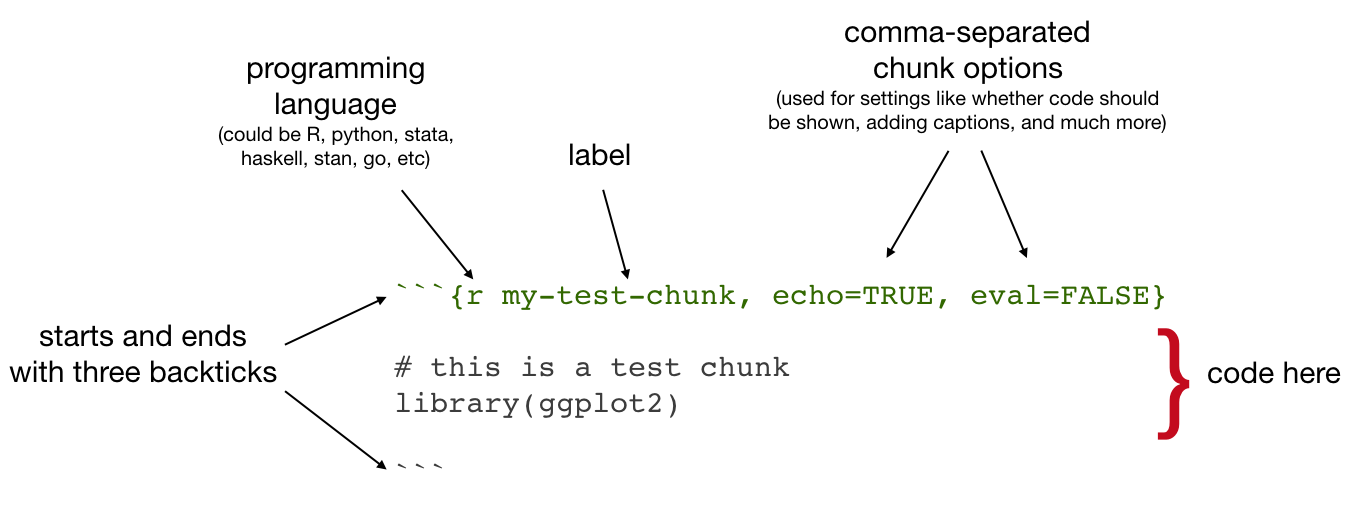
\includegraphics[width=1\linewidth]{figures/sample-content/chunk-parts} \caption{Code chunk syntax}\label{fig:chunk-parts}
\end{figure}

Common chunk options include (see e.g.~\href{https://bookdown.org/yihui/rmarkdown/r-code.html}{bookdown.org}):

\begin{itemize}
\tightlist
\item
  \texttt{echo}: whether or not to display code in knitted output
\item
  \texttt{eval}: whether or to to run the code in the chunk when knitting
\item
  \texttt{include}: whether to include anything from the from a code chunk in the output document
\item
  \texttt{fig.cap}: figure caption
\item
  \texttt{fig.scap}: short figure caption, which will be used in the `List of Figures' in the PDF front matter
\end{itemize}

\textbf{IMPORTANT}: Do \emph{not} use underscoores in your chunk labels - if you do, you are likely to get an error in PDF output saying something like ``! Package caption Error: \textbackslash caption outside float''.

\hypertarget{setup-chunks---setup-images-plots}{%
\subsection{Setup chunks - setup, images, plots}\label{setup-chunks---setup-images-plots}}

An R Markdown document usually begins with a chunk that is used to \textbf{load libraries}, and to \textbf{set default chunk options} with \texttt{knitr::opts\_chunk\$set}.

In your thesis, this will probably happen in \textbf{index.Rmd} and/or as opening chunks in each of your chapters.

\begin{verbatim}
```{r setup, include=FALSE}
# don't show code unless we explicitly set echo = TRUE
knitr::opts_chunk$set(echo = FALSE)

library(tidyverse)
```
\end{verbatim}

\hypertarget{including-images}{%
\subsection{Including images}\label{including-images}}

Code chunks are also used for including images, with \texttt{include\_graphics} from the \texttt{knitr} package, as in Figure \ref{fig:oxford-logo}

\begin{Shaded}
\begin{Highlighting}[]
\NormalTok{knitr}\OperatorTok{::}\KeywordTok{include\_graphics}\NormalTok{(}\StringTok{"figures/sample{-}content/beltcrest.png"}\NormalTok{)}
\end{Highlighting}
\end{Shaded}

\begin{figure}

{\centering 
\includegraphics[width=0.5\linewidth]{figures/sample-content/beltcrest} 

}

\caption{Oxford logo}\label{fig:oxford-logo}
\end{figure}

Useful chunk options for figures include:

\begin{itemize}
\tightlist
\item
  \texttt{out.width} (use with a percentage) for setting the image size
\item
  if you've got an image that gets waaay to big in your output, it will be constrained to the page width by setting \texttt{out.width\ =\ "100\%"}
\end{itemize}

\hypertarget{figure-rotation}{%
\subsubsection*{Figure rotation}\label{figure-rotation}}
\addcontentsline{toc}{subsubsection}{Figure rotation}

You can use the chunk option \texttt{out.extra} to rotate images.

The syntax is different for LaTeX and HTML, so for ease we might start by assigning the right string to a variable that depends on the format you're outputting to:

\begin{Shaded}
\begin{Highlighting}[]
\ControlFlowTok{if}\NormalTok{ (knitr}\OperatorTok{::}\KeywordTok{is\_latex\_output}\NormalTok{())\{}
\NormalTok{  rotate180 \textless{}{-}}\StringTok{ "angle=180"}
\NormalTok{\} }\ControlFlowTok{else}\NormalTok{ \{}
\NormalTok{  rotate180 \textless{}{-}}\StringTok{ "style=\textquotesingle{}transform:rotate(180deg);\textquotesingle{}"}
\NormalTok{\}}
\end{Highlighting}
\end{Shaded}

Then you can reference that variable as the value of \texttt{out.extra} to rotate images, as in Figure \ref{fig:oxford-logo-rotated}.

\begin{figure}

{\centering 
\includegraphics[width=0.5\linewidth,angle=180]{figures/sample-content/beltcrest} 

}

\caption{Oxford logo, rotated}\label{fig:oxford-logo-rotated}
\end{figure}

\hypertarget{including-plots}{%
\subsection{Including plots}\label{including-plots}}

Similarly, code chunks are used for including dynamically generated plots.
You use ordinary code in R or other languages - Figure \ref{fig:cars-plot} shows a plot of the \texttt{cars} dataset of stopping distances for cars at various speeds (this dataset is built in to \textbf{R}).

\begin{Shaded}
\begin{Highlighting}[]
\NormalTok{cars }\OperatorTok{\%\textgreater{}\%}\StringTok{ }
\StringTok{  }\KeywordTok{ggplot}\NormalTok{() }\OperatorTok{+}
\StringTok{    }\KeywordTok{aes}\NormalTok{(}\DataTypeTok{x =}\NormalTok{ speed, }\DataTypeTok{y =}\NormalTok{ dist) }\OperatorTok{+}
\StringTok{    }\KeywordTok{geom\_point}\NormalTok{()}
\end{Highlighting}
\end{Shaded}

\begin{figure}
\centering
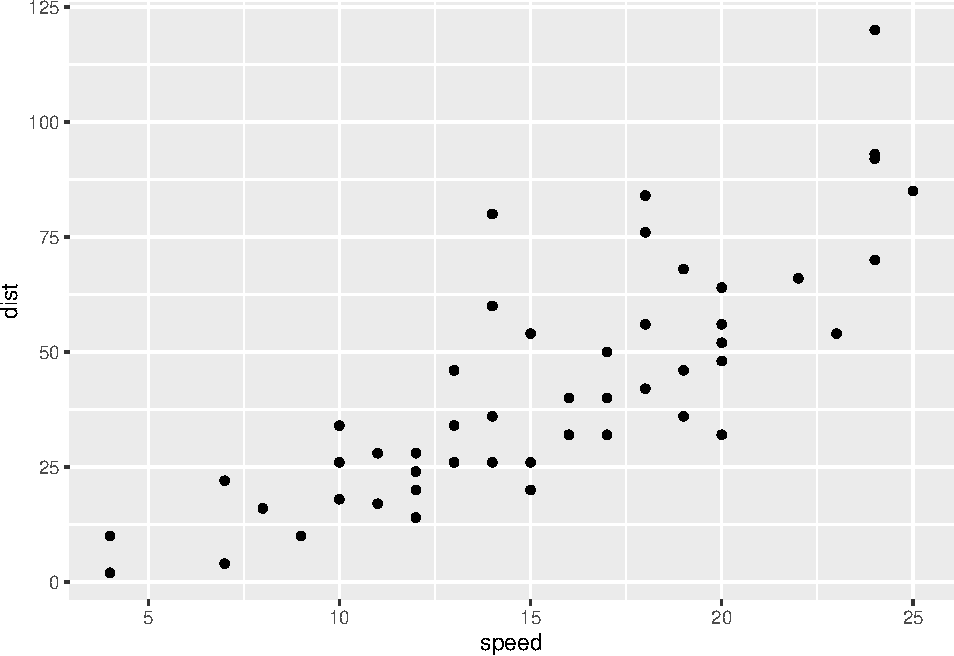
\includegraphics{_main_files/figure-latex/cars-plot-1.pdf}
\caption{\label{fig:cars-plot}A ggplot of car stuff}
\end{figure}

Under the hood, plots are included in your document in the same way as images - when you build the book or knit a chapter, the plot is automatically generated from your code, saved as an image, then included into the output document.

\hypertarget{including-tables}{%
\subsection{Including tables}\label{including-tables}}

Tables are usually included with the \texttt{kable} function from the \texttt{knitr} package.

Table \ref{tab:cars-table} shows the first rows of that cars data - read in your own data, then use this approach to automatically generate tables.

\begin{Shaded}
\begin{Highlighting}[]
\NormalTok{cars }\OperatorTok{\%\textgreater{}\%}\StringTok{ }
\StringTok{  }\KeywordTok{head}\NormalTok{() }\OperatorTok{\%\textgreater{}\%}\StringTok{ }
\StringTok{  }\NormalTok{knitr}\OperatorTok{::}\KeywordTok{kable}\NormalTok{(}\DataTypeTok{caption =} \StringTok{"A knitr kable table"}\NormalTok{)}
\end{Highlighting}
\end{Shaded}

\begin{table}

\caption{\label{tab:cars-table}A knitr kable table}
\centering
\begin{tabular}[t]{r|r}
\hline
speed & dist\\
\hline
4 & 2\\
\hline
4 & 10\\
\hline
7 & 4\\
\hline
7 & 22\\
\hline
8 & 16\\
\hline
9 & 10\\
\hline
\end{tabular}
\end{table}

\begin{itemize}
\tightlist
\item
  Gotcha: when using \href{https://www.rdocumentation.org/packages/knitr/versions/1.21/topics/kable}{\texttt{kable}}, captions are set inside the \texttt{kable} function
\item
  The \texttt{kable} package is often used with the \href{https://cran.r-project.org/web/packages/kableExtra/vignettes/awesome_table_in_html.html}{\texttt{kableExtra}} package
\end{itemize}

\hypertarget{control-positioning}{%
\subsection{Control positioning}\label{control-positioning}}

One thing that may be annoying is the way \emph{R Markdown} handles ``floats'' like tables and figures.
In your PDF output, LaTeX will try to find the best place to put your object based on the text around it and until you're really, truly done writing you should just leave it where it lies.

In general, you should allow LaTeX to do this, but if you really \emph{really} need a figure to be positioned where you put in the document, then you can make LaTeX attempt to do this with the chunk option \texttt{fig.pos="H"}, as in Figure \ref{fig:oxford-logo-controlled}:

\begin{Shaded}
\begin{Highlighting}[]
\NormalTok{knitr}\OperatorTok{::}\KeywordTok{include\_graphics}\NormalTok{(}\StringTok{"figures/sample{-}content/beltcrest.png"}\NormalTok{)}
\end{Highlighting}
\end{Shaded}

\begin{figure}[H]

{\centering 
\includegraphics[width=0.5\linewidth]{figures/sample-content/beltcrest} 

}

\caption{An Oxford logo that LaTeX will try to place at this position in the text}\label{fig:oxford-logo-controlled}
\end{figure}

As anyone who has tried to manually play around with the placement of figures in a Word document knows, this can have lots of side effects with extra spacing on other pages, etc.
Therefore, it is not generally a good idea to do this - only do it when you really need to ensure that an image follows directly under text where you refer to it (in this document, I needed to do this for Figure \ref{fig:latex-font-sizing} in section \ref{max-power}).
For more details, read the relevant section of the \href{https://bookdown.org/yihui/rmarkdown-cookbook/figure-placement.html}{R Markdown Cookbook}.

\hypertarget{executable-inline-code}{%
\section{Executable inline code}\label{executable-inline-code}}

`Inline code' simply means inclusion of code inside text.
The syntax for doing this is \texttt{\textasciigrave{}r\ R\_CODE\textasciigrave{}}
For example, \texttt{\textasciigrave{}r\ 4\ +\ 4\textasciigrave{}} will output 8 in your text.

You will usually use this in parts of your thesis where you report results - read in data or results in a code chunk, store things you want to report in a variable, then insert the value of that variable in your text.
For example, we might assign the number of rows in the \texttt{cars} dataset to a variable:

\begin{Shaded}
\begin{Highlighting}[]
\NormalTok{num\_car\_observations \textless{}{-}}\StringTok{ }\KeywordTok{nrow}\NormalTok{(cars)}
\end{Highlighting}
\end{Shaded}

We might then write:\\
``In the \texttt{cars} dataset, we have \texttt{\textasciigrave{}r\ num\_car\_observations\textasciigrave{}} observations.''

Which would output:\\
``In the \texttt{cars} dataset, we have 50 observations.''

\hypertarget{executable-code-in-other-languages-than-r}{%
\section{Executable code in other languages than R}\label{executable-code-in-other-languages-than-r}}

If you want to use other languages than R, such as Python, Julia C++, or SQL, see \href{https://bookdown.org/yihui/rmarkdown-cookbook/other-languages.html}{the relevant section of the \emph{R Markdown Cookbook}}

\hypertarget{cites-and-refs}{%
\chapter{Citations, cross-references, and collaboration}\label{cites-and-refs}}

\chaptermark{Citations and cross-refs}

\minitoc 

\hypertarget{citations}{%
\section{Citations}\label{citations}}

The usual way to include citations in an \emph{R Markdown} document is to put references in a plain text file with the extension \textbf{.bib}, in \textbf{BibTex} format.\footnote{The bibliography can be in other formats as well, including EndNote (\textbf{.enl}) and RIS (\textbf{.ris}), see \href{https://rmarkdown.rstudio.com/authoring_bibliographies_and_citations.html}{rmarkdown.rstudio.com/authoring\_bibliographies\_and\_citations}.}
Then reference the path to this file in \textbf{index.Rmd}'s YAML header with \texttt{bibliography:\ example.bib}.

Most reference managers can create a .bib file with you references automatically.
However, the \textbf{by far} best reference manager to use with \emph{R Markdown} is \href{https://www.zotero.org}{Zotero} with the \href{https://retorque.re/zotero-better-bibtex/}{Better BibTex plug-in}, because the \texttt{citr} plugin for RStudio (see below) can read references directly from your Zotero library!

Here is an example of an entry in a \textbf{.bib} file:

\begin{Shaded}
\begin{Highlighting}[]
\VariableTok{@article}\NormalTok{\{}\OtherTok{Shea2014}\NormalTok{,}
  \DataTypeTok{author}\NormalTok{ =        \{Shea, Nicholas and Boldt, Annika\},}
  \DataTypeTok{journal}\NormalTok{ =       \{Trends in Cognitive Sciences\},}
  \DataTypeTok{pages}\NormalTok{ =         \{186{-}{-}193\},}
  \DataTypeTok{title}\NormalTok{ =         \{\{Supra{-}personal cognitive control\}\},}
  \DataTypeTok{volume}\NormalTok{ =        \{18\},}
  \DataTypeTok{year}\NormalTok{ =          \{2014\},}
  \DataTypeTok{doi}\NormalTok{ =           \{10.1016/j.tics.2014.01.006\},}
\NormalTok{\}}
\end{Highlighting}
\end{Shaded}

In this entry highlighed section, `Shea2014' is the \textbf{citation identifier}.
To default way to cite an entry in your text is with this syntax: \texttt{{[}@citation-identifier{]}}.

So I might cite some things \autocite{Shea2014,Lottridge2012}.

\hypertarget{pdf-output}{%
\subsection{PDF output}\label{pdf-output}}

In PDF output, the bibliography is handled by the OxThesis LaTeX template.
If you set \texttt{bib-humanities:\ true} in \textbf{index.Rmd}, then in-text references will be formatted as author-year; otherwise references will be shown as numbers.

If you choose author-year formatting, a number of variations on the citation syntax are useful to know:

\begin{itemize}
\tightlist
\item
  Put author names outside the parenthesis

  \begin{itemize}
  \tightlist
  \item
    This: \texttt{@Shea2014\ says\ blah.}
  \item
    Becomes: \textcite{Shea2014} says blah.
  \end{itemize}
\item
  Include only the citation-year (in parenthesis)

  \begin{itemize}
  \tightlist
  \item
    This: \texttt{Shea\ et\ al.\ says\ blah\ {[}-@Shea2014{]}}
  \item
    Becomes: Shea et al.~says blah \autocite*{Shea2014}
  \end{itemize}
\item
  Add text and page or chapter references to the citation

  \begin{itemize}
  \tightlist
  \item
    This: \texttt{{[}see\ @Shea2014,\ pp.\ 33-35;\ also\ @Wu2016,\ ch.\ 1{]}}
  \item
    Becomes: Blah blah \autocites[see][pp.~33-35]{Shea2014}[also][ch.~1]{Wu2016}.
  \end{itemize}
\end{itemize}

\hypertarget{gitbook-output}{%
\subsection{Gitbook output}\label{gitbook-output}}

In gitbook output, citations are by default inserted in the Chicago author-date format.

To change the format, add \texttt{csl:\ some-other-style.csl} in \textbf{index.Rmd}'s YAML header.
You can browse through and download styles at \href{https://www.zotero.org/styles}{zotero.org/styles}.

\clearpage

\hypertarget{insert-references-easily-with-the-citr-add-in}{%
\subsection{\texorpdfstring{Insert references easily with the \texttt{citr} add-in}{Insert references easily with the citr add-in}}\label{insert-references-easily-with-the-citr-add-in}}

For an easy way to insert citations, try the \href{https://github.com/crsh/citr}{\texttt{citr}} RStudio add-in (Figure \ref{fig:citr}).
You can install this add-in by typing \texttt{install.packages("citr")} in the R Console.

\begin{figure}

{\centering 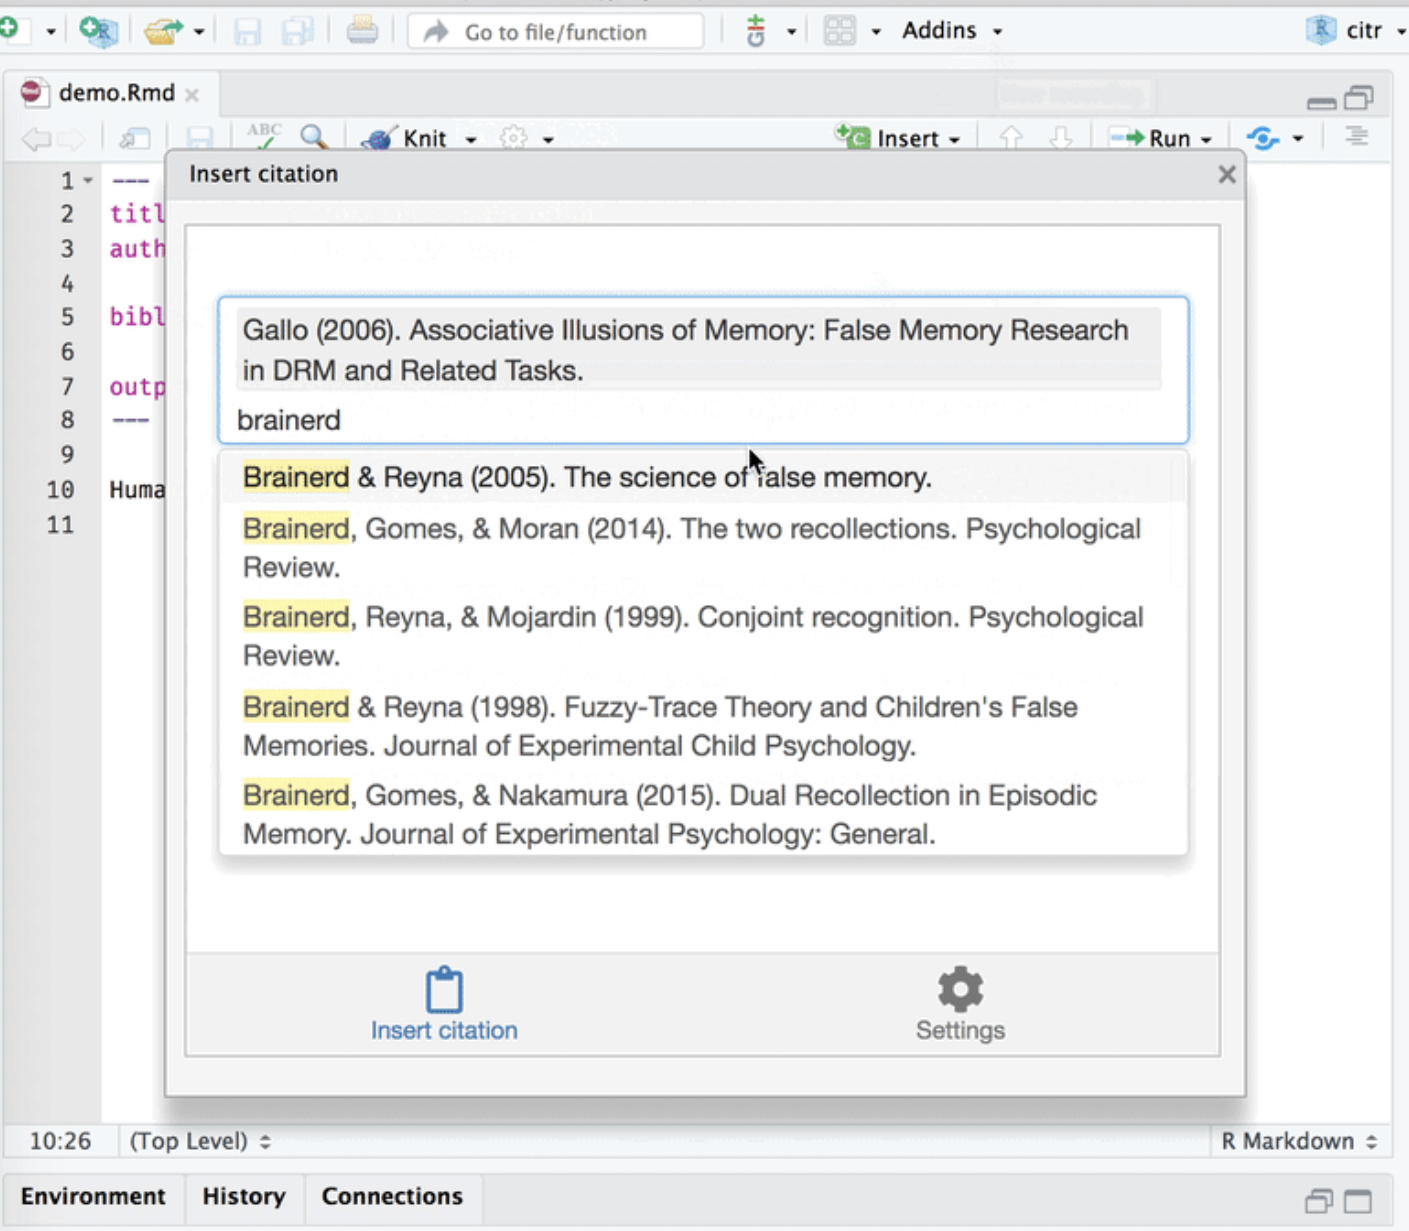
\includegraphics[width=0.8\linewidth]{figures/sample-content/citr} 

}

\caption{The `citr` add-in}\label{fig:citr}
\end{figure}

\hypertarget{cross-referencing}{%
\section{Cross-referencing}\label{cross-referencing}}

We can make cross-references to \textbf{sections} within our document, as well as to \textbf{figures} (images and plots) and \textbf{tables}.

The general cross-referencing syntax is \textbf{\texttt{\textbackslash{}@ref(label)}}

\hypertarget{section-references}{%
\subsection{Section references}\label{section-references}}

Headers are automatically assigned a reference label, which is the text in lower caps separated by dashes. For example, \texttt{\#\ My\ header} is automatically given the label \texttt{my-header}. So \texttt{\#\ My\ header} can be referenced with \texttt{\textbackslash{}@ref(my-section)}

Remember what we wrote in section \ref{citations}?

We can also use \textbf{hyperlink syntax} and add \# before the label, though this is only guaranteed to work properly in HTML output:

\begin{itemize}
\tightlist
\item
  So if we write \texttt{Remember\ what\ we\ wrote\ up\ in\ {[}the\ previous\ section{]}(\#citations)?}
\item
  It becomes Remember what we wrote up in \protect\hyperlink{citations}{the previous section}?
\end{itemize}

\hypertarget{creating-custom-labels}{%
\subsubsection{Creating custom labels}\label{creating-custom-labels}}

It is a very good idea to create \textbf{custom labels} for our sections. This is because the automatically assigned labels will change when we change the titles of the sections - to avoid this, we can create the labels ourselves and leave them untouched if we change the section titles.

We create custom labels by adding \texttt{\{\#label\}} after a header, e.g.~\texttt{\#\ My\ section\ \{\#my-label\}}.
See \protect\hyperlink{cites-and-refs}{our chapter title} for an example. That was section \ref{cites-and-refs}.

\hypertarget{figure-image-and-plot-references}{%
\subsection{Figure (image and plot) references}\label{figure-image-and-plot-references}}

\begin{itemize}
\tightlist
\item
  To refer to figures (i.e.~images and plots) use the syntax \texttt{\textbackslash{}@ref(fig:label)}
\item
  \textbf{GOTCHA}: Figures and tables must have captions if you wish to cross-reference them.
\end{itemize}

Let's add an image:

\begin{Shaded}
\begin{Highlighting}[]
\NormalTok{knitr}\OperatorTok{::}\KeywordTok{include\_graphics}\NormalTok{(}\StringTok{"figures/sample{-}content/captain.jpeg"}\NormalTok{)}
\end{Highlighting}
\end{Shaded}

\begin{figure}

{\centering 
\includegraphics[width=0.65\linewidth]{figures/sample-content/captain} 

}

\caption{A marvel-lous meme}\label{fig:captain}
\end{figure}

We refer to this image with \texttt{\textbackslash{}@ref(fig:captain)}.
So Figure \ref{fig:captain} is \protect\hyperlink{fig:captain}{this image}.

And in Figure \ref{fig:cars-plot} we saw a \protect\hyperlink{fig:cars-plot}{cars plot}.

\hypertarget{table-references}{%
\subsection{Table references}\label{table-references}}

\begin{itemize}
\tightlist
\item
  To refer to tables use the syntax \texttt{\textbackslash{}@ref(tab:label)}
\end{itemize}

Let's include a table:

\begin{Shaded}
\begin{Highlighting}[]
\NormalTok{knitr}\OperatorTok{::}\KeywordTok{kable}\NormalTok{(cars[}\DecValTok{1}\OperatorTok{:}\DecValTok{5}\NormalTok{,],}
            \DataTypeTok{caption=}\StringTok{"Stopping cars"}\NormalTok{)}
\end{Highlighting}
\end{Shaded}

\begin{table}

\caption{\label{tab:cars-table2}Stopping cars}
\centering
\begin{tabular}[t]{r|r}
\hline
speed & dist\\
\hline
4 & 2\\
\hline
4 & 10\\
\hline
7 & 4\\
\hline
7 & 22\\
\hline
8 & 16\\
\hline
\end{tabular}
\end{table}

We refer to this table with \texttt{\textbackslash{}@ref(tab:cars-table2)}.
So Table \ref{tab:cars-table2} is \protect\hyperlink{tab:cars-table2}{this table}.

And in Table \ref{tab:cars-table} we saw more or less \protect\hyperlink{tab:cars-table}{the same cars table}.

\hypertarget{including-page-numbers}{%
\subsection{Including page numbers}\label{including-page-numbers}}

Finally, in the PDF output we might also want to include the page number of a reference, so that it's easy to find in physical printed output.
LaTeX has a command for this, which looks like this: \texttt{\textbackslash{}pageref\{fig/tab:label\}} (note: curly braces, not parentheses)

When we output to PDF, we can use raw LaTeX directly in our .Rmd files. So if we wanted to include the page of the cars plot we could write:

\begin{itemize}
\tightlist
\item
  This: \texttt{Figure\ \textbackslash{}@ref(fig:cars-plot)\ on\ page\ \textbackslash{}pageref(fig:cars-plot)}
\item
  Becomes: Figure \ref{fig:cars-plot} on page \pageref{fig:cars-plot}
\end{itemize}

\hypertarget{include-page-numbers-only-in-pdf-output}{%
\subsubsection{Include page numbers only in PDF output}\label{include-page-numbers-only-in-pdf-output}}

A problem here is that LaTeX commands don't display in HTML output, so in the gitbook output we'd see simply ``Figure \ref{fig:cars-plot} on page''.

One way to get around this is to use inline R code to insert the text, and use an \texttt{ifelse} statement to check the output format and then insert the appropriate text.

\begin{itemize}
\tightlist
\item
  So this: \texttt{\textasciigrave{}r\ ifelse(knitr::is\_latex\_output(),\ "Figure\ \textbackslash{}\textbackslash{}@ref(fig:cars-plot)\ on\ page\ \textbackslash{}\textbackslash{}pageref\{fig:cars-plot\}",\ "")\textasciigrave{}}
\item
  Inserts this (check this on both PDF and gitbook): Figure \ref{fig:cars-plot} on page \pageref{fig:cars-plot}
\end{itemize}

Note that we need to escape the backslash with another backslash here to get the correct output.

\hypertarget{collaborative-writing}{%
\section{Collaborative writing}\label{collaborative-writing}}

Best practices for collaboration and change tracking when using R Markdown are still an open question.
In the blog post \href{https://livefreeordichotomize.com/2018/09/14/one-year-to-dissertate/}{\textbf{One year to dissertate}} by Lucy D'Agostino, which I highly recommend, the author notes that she knits .Rmd files to a word document, then uses the \texttt{googledrive} R package to send this to Google Drive for comments / revisions from co-authors, then incorporates Google Drive suggestions \emph{by hand} into the .Rmd source files.
This is a bit clunky, and there are ongoing discussions among the \emph{R Markdown} developers about what the best way is to handle collaborative writing (see \href{https://github.com/rstudio/rmarkdown/issues/1463}{issue \#1463} on GitHub, where \href{http://criticmarkup.com}{CriticMarkup} is among the suggestions).

For now, this is an open question in the community of R Markdown users.
I often knit to a format that can easily be imported to Google Docs for comments, then go over suggested revisions and manually incorporate them back in to the .Rmd source files.
For articles, I sometimes upload a near-final draft to \href{https://www.overleaf.com/}{Overleaf}, then collaboratively make final edits to the LaTeX file there.
I suspect some great solution will be developed in the not-to-distant future, probably by the RStudio team.

\hypertarget{additional-resources}{%
\section{Additional resources}\label{additional-resources}}

\begin{itemize}
\item
  \emph{R Markdown: The Definitive Guide} - \url{https://bookdown.org/yihui/rmarkdown/}
\item
  \emph{R for Data Science} - \url{https://r4ds.had.co.nz}
\end{itemize}

\hypertarget{tables}{%
\chapter{Tables}\label{tables}}

\minitoc 

\hypertarget{making-latex-tables-play-nice}{%
\section{Making LaTeX tables play nice}\label{making-latex-tables-play-nice}}

Dealing with tables in LaTeX can be painful.
This section explains the main tricks you need to make the pain go away.

(Note: if you are looking at the ebook version, you will not see much difference in this section, as it is only relevant for PDF output!)

\hypertarget{making-your-table-pretty}{%
\subsection{Making your table pretty}\label{making-your-table-pretty}}

When you use \texttt{kable} to create tables, you will almost certainly want to set the option \texttt{booktabs\ =\ TRUE}.
This makes your table look a million times better:

\begin{Shaded}
\begin{Highlighting}[]
\KeywordTok{library}\NormalTok{(knitr)}
\KeywordTok{library}\NormalTok{(tidyverse)}

\KeywordTok{head}\NormalTok{(mtcars) }\OperatorTok{\%\textgreater{}\%}\StringTok{ }
\StringTok{  }\KeywordTok{kable}\NormalTok{(}\DataTypeTok{booktabs =} \OtherTok{TRUE}\NormalTok{)}
\end{Highlighting}
\end{Shaded}

\begin{tabular}{lrrrrrrrrrrr}
\toprule
  & mpg & cyl & disp & hp & drat & wt & qsec & vs & am & gear & carb\\
\midrule
Mazda RX4 & 21.0 & 6 & 160 & 110 & 3.90 & 2.620 & 16.46 & 0 & 1 & 4 & 4\\
Mazda RX4 Wag & 21.0 & 6 & 160 & 110 & 3.90 & 2.875 & 17.02 & 0 & 1 & 4 & 4\\
Datsun 710 & 22.8 & 4 & 108 & 93 & 3.85 & 2.320 & 18.61 & 1 & 1 & 4 & 1\\
Hornet 4 Drive & 21.4 & 6 & 258 & 110 & 3.08 & 3.215 & 19.44 & 1 & 0 & 3 & 1\\
Hornet Sportabout & 18.7 & 8 & 360 & 175 & 3.15 & 3.440 & 17.02 & 0 & 0 & 3 & 2\\
\addlinespace
Valiant & 18.1 & 6 & 225 & 105 & 2.76 & 3.460 & 20.22 & 1 & 0 & 3 & 1\\
\bottomrule
\end{tabular}

\vspace{4mm}

Compare this to the default style, which looks terrible:

\begin{Shaded}
\begin{Highlighting}[]
\KeywordTok{head}\NormalTok{(mtcars) }\OperatorTok{\%\textgreater{}\%}\StringTok{ }
\StringTok{  }\KeywordTok{kable}\NormalTok{()}
\end{Highlighting}
\end{Shaded}

\begin{tabular}{l|r|r|r|r|r|r|r|r|r|r|r}
\hline
  & mpg & cyl & disp & hp & drat & wt & qsec & vs & am & gear & carb\\
\hline
Mazda RX4 & 21.0 & 6 & 160 & 110 & 3.90 & 2.620 & 16.46 & 0 & 1 & 4 & 4\\
\hline
Mazda RX4 Wag & 21.0 & 6 & 160 & 110 & 3.90 & 2.875 & 17.02 & 0 & 1 & 4 & 4\\
\hline
Datsun 710 & 22.8 & 4 & 108 & 93 & 3.85 & 2.320 & 18.61 & 1 & 1 & 4 & 1\\
\hline
Hornet 4 Drive & 21.4 & 6 & 258 & 110 & 3.08 & 3.215 & 19.44 & 1 & 0 & 3 & 1\\
\hline
Hornet Sportabout & 18.7 & 8 & 360 & 175 & 3.15 & 3.440 & 17.02 & 0 & 0 & 3 & 2\\
\hline
Valiant & 18.1 & 6 & 225 & 105 & 2.76 & 3.460 & 20.22 & 1 & 0 & 3 & 1\\
\hline
\end{tabular}

\hypertarget{if-your-table-is-too-wide}{%
\subsection{If your table is too wide}\label{if-your-table-is-too-wide}}

You might find that your table expands into the margins of the page, like the tables above.
Fix this with the \texttt{kable\_styling} function from the \href{https://haozhu233.github.io/kableExtra/}{\texttt{kableExtra}} package:

\begin{Shaded}
\begin{Highlighting}[]
\KeywordTok{library}\NormalTok{(kableExtra)}

\KeywordTok{head}\NormalTok{(mtcars) }\OperatorTok{\%\textgreater{}\%}\StringTok{ }
\StringTok{  }\KeywordTok{kable}\NormalTok{(}\DataTypeTok{booktabs =} \OtherTok{TRUE}\NormalTok{) }\OperatorTok{\%\textgreater{}\%}\StringTok{ }
\StringTok{  }\KeywordTok{kable\_styling}\NormalTok{(}\DataTypeTok{latex\_options =} \StringTok{"scale\_down"}\NormalTok{)}
\end{Highlighting}
\end{Shaded}

\begin{table}[H]
\centering
\resizebox{\linewidth}{!}{
\begin{tabular}{lrrrrrrrrrrr}
\toprule
  & mpg & cyl & disp & hp & drat & wt & qsec & vs & am & gear & carb\\
\midrule
Mazda RX4 & 21.0 & 6 & 160 & 110 & 3.90 & 2.620 & 16.46 & 0 & 1 & 4 & 4\\
Mazda RX4 Wag & 21.0 & 6 & 160 & 110 & 3.90 & 2.875 & 17.02 & 0 & 1 & 4 & 4\\
Datsun 710 & 22.8 & 4 & 108 & 93 & 3.85 & 2.320 & 18.61 & 1 & 1 & 4 & 1\\
Hornet 4 Drive & 21.4 & 6 & 258 & 110 & 3.08 & 3.215 & 19.44 & 1 & 0 & 3 & 1\\
Hornet Sportabout & 18.7 & 8 & 360 & 175 & 3.15 & 3.440 & 17.02 & 0 & 0 & 3 & 2\\
\addlinespace
Valiant & 18.1 & 6 & 225 & 105 & 2.76 & 3.460 & 20.22 & 1 & 0 & 3 & 1\\
\bottomrule
\end{tabular}}
\end{table}

This scales down the table to fit the page width.

\hypertarget{if-your-table-is-too-long}{%
\subsection{If your table is too long}\label{if-your-table-is-too-long}}

If your table is too long to fit on a single page, set \texttt{longtable\ =\ TRUE} in the \texttt{kable} function to split the table across multiple pages.

\begin{Shaded}
\begin{Highlighting}[]
\NormalTok{a\_long\_table \textless{}{-}}\StringTok{ }\KeywordTok{rbind}\NormalTok{(mtcars, mtcars)}

\NormalTok{a\_long\_table }\OperatorTok{\%\textgreater{}\%}\StringTok{ }
\StringTok{  }\KeywordTok{select}\NormalTok{(}\DecValTok{1}\OperatorTok{:}\DecValTok{8}\NormalTok{) }\OperatorTok{\%\textgreater{}\%}\StringTok{ }
\StringTok{  }\KeywordTok{kable}\NormalTok{(}\DataTypeTok{booktabs =} \OtherTok{TRUE}\NormalTok{, }\DataTypeTok{longtable =} \OtherTok{TRUE}\NormalTok{)}
\end{Highlighting}
\end{Shaded}

\begin{longtable}{lrrrrrrrr}
\toprule
  & mpg & cyl & disp & hp & drat & wt & qsec & vs\\
\midrule
Mazda RX4 & 21.0 & 6 & 160.0 & 110 & 3.90 & 2.620 & 16.46 & 0\\
Mazda RX4 Wag & 21.0 & 6 & 160.0 & 110 & 3.90 & 2.875 & 17.02 & 0\\
Datsun 710 & 22.8 & 4 & 108.0 & 93 & 3.85 & 2.320 & 18.61 & 1\\
Hornet 4 Drive & 21.4 & 6 & 258.0 & 110 & 3.08 & 3.215 & 19.44 & 1\\
Hornet Sportabout & 18.7 & 8 & 360.0 & 175 & 3.15 & 3.440 & 17.02 & 0\\
\addlinespace
Valiant & 18.1 & 6 & 225.0 & 105 & 2.76 & 3.460 & 20.22 & 1\\
Duster 360 & 14.3 & 8 & 360.0 & 245 & 3.21 & 3.570 & 15.84 & 0\\
Merc 240D & 24.4 & 4 & 146.7 & 62 & 3.69 & 3.190 & 20.00 & 1\\
Merc 230 & 22.8 & 4 & 140.8 & 95 & 3.92 & 3.150 & 22.90 & 1\\
Merc 280 & 19.2 & 6 & 167.6 & 123 & 3.92 & 3.440 & 18.30 & 1\\
\addlinespace
Merc 280C & 17.8 & 6 & 167.6 & 123 & 3.92 & 3.440 & 18.90 & 1\\
Merc 450SE & 16.4 & 8 & 275.8 & 180 & 3.07 & 4.070 & 17.40 & 0\\
Merc 450SL & 17.3 & 8 & 275.8 & 180 & 3.07 & 3.730 & 17.60 & 0\\
Merc 450SLC & 15.2 & 8 & 275.8 & 180 & 3.07 & 3.780 & 18.00 & 0\\
Cadillac Fleetwood & 10.4 & 8 & 472.0 & 205 & 2.93 & 5.250 & 17.98 & 0\\
\addlinespace
Lincoln Continental & 10.4 & 8 & 460.0 & 215 & 3.00 & 5.424 & 17.82 & 0\\
Chrysler Imperial & 14.7 & 8 & 440.0 & 230 & 3.23 & 5.345 & 17.42 & 0\\
Fiat 128 & 32.4 & 4 & 78.7 & 66 & 4.08 & 2.200 & 19.47 & 1\\
Honda Civic & 30.4 & 4 & 75.7 & 52 & 4.93 & 1.615 & 18.52 & 1\\
Toyota Corolla & 33.9 & 4 & 71.1 & 65 & 4.22 & 1.835 & 19.90 & 1\\
\addlinespace
Toyota Corona & 21.5 & 4 & 120.1 & 97 & 3.70 & 2.465 & 20.01 & 1\\
Dodge Challenger & 15.5 & 8 & 318.0 & 150 & 2.76 & 3.520 & 16.87 & 0\\
AMC Javelin & 15.2 & 8 & 304.0 & 150 & 3.15 & 3.435 & 17.30 & 0\\
Camaro Z28 & 13.3 & 8 & 350.0 & 245 & 3.73 & 3.840 & 15.41 & 0\\
Pontiac Firebird & 19.2 & 8 & 400.0 & 175 & 3.08 & 3.845 & 17.05 & 0\\
\addlinespace
Fiat X1-9 & 27.3 & 4 & 79.0 & 66 & 4.08 & 1.935 & 18.90 & 1\\
Porsche 914-2 & 26.0 & 4 & 120.3 & 91 & 4.43 & 2.140 & 16.70 & 0\\
Lotus Europa & 30.4 & 4 & 95.1 & 113 & 3.77 & 1.513 & 16.90 & 1\\
Ford Pantera L & 15.8 & 8 & 351.0 & 264 & 4.22 & 3.170 & 14.50 & 0\\
Ferrari Dino & 19.7 & 6 & 145.0 & 175 & 3.62 & 2.770 & 15.50 & 0\\
\addlinespace
Maserati Bora & 15.0 & 8 & 301.0 & 335 & 3.54 & 3.570 & 14.60 & 0\\
Volvo 142E & 21.4 & 4 & 121.0 & 109 & 4.11 & 2.780 & 18.60 & 1\\
Mazda RX41 & 21.0 & 6 & 160.0 & 110 & 3.90 & 2.620 & 16.46 & 0\\
Mazda RX4 Wag1 & 21.0 & 6 & 160.0 & 110 & 3.90 & 2.875 & 17.02 & 0\\
Datsun 7101 & 22.8 & 4 & 108.0 & 93 & 3.85 & 2.320 & 18.61 & 1\\
\addlinespace
Hornet 4 Drive1 & 21.4 & 6 & 258.0 & 110 & 3.08 & 3.215 & 19.44 & 1\\
Hornet Sportabout1 & 18.7 & 8 & 360.0 & 175 & 3.15 & 3.440 & 17.02 & 0\\
Valiant1 & 18.1 & 6 & 225.0 & 105 & 2.76 & 3.460 & 20.22 & 1\\
Duster 3601 & 14.3 & 8 & 360.0 & 245 & 3.21 & 3.570 & 15.84 & 0\\
Merc 240D1 & 24.4 & 4 & 146.7 & 62 & 3.69 & 3.190 & 20.00 & 1\\
\addlinespace
Merc 2301 & 22.8 & 4 & 140.8 & 95 & 3.92 & 3.150 & 22.90 & 1\\
Merc 2801 & 19.2 & 6 & 167.6 & 123 & 3.92 & 3.440 & 18.30 & 1\\
Merc 280C1 & 17.8 & 6 & 167.6 & 123 & 3.92 & 3.440 & 18.90 & 1\\
Merc 450SE1 & 16.4 & 8 & 275.8 & 180 & 3.07 & 4.070 & 17.40 & 0\\
Merc 450SL1 & 17.3 & 8 & 275.8 & 180 & 3.07 & 3.730 & 17.60 & 0\\
\addlinespace
Merc 450SLC1 & 15.2 & 8 & 275.8 & 180 & 3.07 & 3.780 & 18.00 & 0\\
Cadillac Fleetwood1 & 10.4 & 8 & 472.0 & 205 & 2.93 & 5.250 & 17.98 & 0\\
Lincoln Continental1 & 10.4 & 8 & 460.0 & 215 & 3.00 & 5.424 & 17.82 & 0\\
Chrysler Imperial1 & 14.7 & 8 & 440.0 & 230 & 3.23 & 5.345 & 17.42 & 0\\
Fiat 1281 & 32.4 & 4 & 78.7 & 66 & 4.08 & 2.200 & 19.47 & 1\\
\addlinespace
Honda Civic1 & 30.4 & 4 & 75.7 & 52 & 4.93 & 1.615 & 18.52 & 1\\
Toyota Corolla1 & 33.9 & 4 & 71.1 & 65 & 4.22 & 1.835 & 19.90 & 1\\
Toyota Corona1 & 21.5 & 4 & 120.1 & 97 & 3.70 & 2.465 & 20.01 & 1\\
Dodge Challenger1 & 15.5 & 8 & 318.0 & 150 & 2.76 & 3.520 & 16.87 & 0\\
AMC Javelin1 & 15.2 & 8 & 304.0 & 150 & 3.15 & 3.435 & 17.30 & 0\\
\addlinespace
Camaro Z281 & 13.3 & 8 & 350.0 & 245 & 3.73 & 3.840 & 15.41 & 0\\
Pontiac Firebird1 & 19.2 & 8 & 400.0 & 175 & 3.08 & 3.845 & 17.05 & 0\\
Fiat X1-91 & 27.3 & 4 & 79.0 & 66 & 4.08 & 1.935 & 18.90 & 1\\
Porsche 914-21 & 26.0 & 4 & 120.3 & 91 & 4.43 & 2.140 & 16.70 & 0\\
Lotus Europa1 & 30.4 & 4 & 95.1 & 113 & 3.77 & 1.513 & 16.90 & 1\\
\addlinespace
Ford Pantera L1 & 15.8 & 8 & 351.0 & 264 & 4.22 & 3.170 & 14.50 & 0\\
Ferrari Dino1 & 19.7 & 6 & 145.0 & 175 & 3.62 & 2.770 & 15.50 & 0\\
Maserati Bora1 & 15.0 & 8 & 301.0 & 335 & 3.54 & 3.570 & 14.60 & 0\\
Volvo 142E1 & 21.4 & 4 & 121.0 & 109 & 4.11 & 2.780 & 18.60 & 1\\
\bottomrule
\end{longtable}

When you do this, you'll probably want to make the header repeat on new pages.
Do this with the \texttt{kable\_styling} function from \texttt{kableExtra}:

\begin{Shaded}
\begin{Highlighting}[]
\NormalTok{a\_long\_table }\OperatorTok{\%\textgreater{}\%}\StringTok{ }
\StringTok{  }\KeywordTok{kable}\NormalTok{(}\DataTypeTok{booktabs =} \OtherTok{TRUE}\NormalTok{, }\DataTypeTok{longtable =} \OtherTok{TRUE}\NormalTok{) }\OperatorTok{\%\textgreater{}\%}\StringTok{ }
\StringTok{  }\KeywordTok{kable\_styling}\NormalTok{(}\DataTypeTok{latex\_options =} \StringTok{"repeat\_header"}\NormalTok{)}
\end{Highlighting}
\end{Shaded}

\begin{longtable}{lrrrrrrrrrrr}
\toprule
  & mpg & cyl & disp & hp & drat & wt & qsec & vs & am & gear & carb\\
\midrule
\endfirsthead
\multicolumn{12}{@{}l}{\textit{(continued)}}\\
\toprule
  & mpg & cyl & disp & hp & drat & wt & qsec & vs & am & gear & carb\\
\midrule
\endhead

\endfoot
\bottomrule
\endlastfoot
Mazda RX4 & 21.0 & 6 & 160.0 & 110 & 3.90 & 2.620 & 16.46 & 0 & 1 & 4 & 4\\
Mazda RX4 Wag & 21.0 & 6 & 160.0 & 110 & 3.90 & 2.875 & 17.02 & 0 & 1 & 4 & 4\\
Datsun 710 & 22.8 & 4 & 108.0 & 93 & 3.85 & 2.320 & 18.61 & 1 & 1 & 4 & 1\\
Hornet 4 Drive & 21.4 & 6 & 258.0 & 110 & 3.08 & 3.215 & 19.44 & 1 & 0 & 3 & 1\\
Hornet Sportabout & 18.7 & 8 & 360.0 & 175 & 3.15 & 3.440 & 17.02 & 0 & 0 & 3 & 2\\
\addlinespace
Valiant & 18.1 & 6 & 225.0 & 105 & 2.76 & 3.460 & 20.22 & 1 & 0 & 3 & 1\\
Duster 360 & 14.3 & 8 & 360.0 & 245 & 3.21 & 3.570 & 15.84 & 0 & 0 & 3 & 4\\
Merc 240D & 24.4 & 4 & 146.7 & 62 & 3.69 & 3.190 & 20.00 & 1 & 0 & 4 & 2\\
Merc 230 & 22.8 & 4 & 140.8 & 95 & 3.92 & 3.150 & 22.90 & 1 & 0 & 4 & 2\\
Merc 280 & 19.2 & 6 & 167.6 & 123 & 3.92 & 3.440 & 18.30 & 1 & 0 & 4 & 4\\
\addlinespace
Merc 280C & 17.8 & 6 & 167.6 & 123 & 3.92 & 3.440 & 18.90 & 1 & 0 & 4 & 4\\
Merc 450SE & 16.4 & 8 & 275.8 & 180 & 3.07 & 4.070 & 17.40 & 0 & 0 & 3 & 3\\
Merc 450SL & 17.3 & 8 & 275.8 & 180 & 3.07 & 3.730 & 17.60 & 0 & 0 & 3 & 3\\
Merc 450SLC & 15.2 & 8 & 275.8 & 180 & 3.07 & 3.780 & 18.00 & 0 & 0 & 3 & 3\\
Cadillac Fleetwood & 10.4 & 8 & 472.0 & 205 & 2.93 & 5.250 & 17.98 & 0 & 0 & 3 & 4\\
\addlinespace
Lincoln Continental & 10.4 & 8 & 460.0 & 215 & 3.00 & 5.424 & 17.82 & 0 & 0 & 3 & 4\\
Chrysler Imperial & 14.7 & 8 & 440.0 & 230 & 3.23 & 5.345 & 17.42 & 0 & 0 & 3 & 4\\
Fiat 128 & 32.4 & 4 & 78.7 & 66 & 4.08 & 2.200 & 19.47 & 1 & 1 & 4 & 1\\
Honda Civic & 30.4 & 4 & 75.7 & 52 & 4.93 & 1.615 & 18.52 & 1 & 1 & 4 & 2\\
Toyota Corolla & 33.9 & 4 & 71.1 & 65 & 4.22 & 1.835 & 19.90 & 1 & 1 & 4 & 1\\
\addlinespace
Toyota Corona & 21.5 & 4 & 120.1 & 97 & 3.70 & 2.465 & 20.01 & 1 & 0 & 3 & 1\\
Dodge Challenger & 15.5 & 8 & 318.0 & 150 & 2.76 & 3.520 & 16.87 & 0 & 0 & 3 & 2\\
AMC Javelin & 15.2 & 8 & 304.0 & 150 & 3.15 & 3.435 & 17.30 & 0 & 0 & 3 & 2\\
Camaro Z28 & 13.3 & 8 & 350.0 & 245 & 3.73 & 3.840 & 15.41 & 0 & 0 & 3 & 4\\
Pontiac Firebird & 19.2 & 8 & 400.0 & 175 & 3.08 & 3.845 & 17.05 & 0 & 0 & 3 & 2\\
\addlinespace
Fiat X1-9 & 27.3 & 4 & 79.0 & 66 & 4.08 & 1.935 & 18.90 & 1 & 1 & 4 & 1\\
Porsche 914-2 & 26.0 & 4 & 120.3 & 91 & 4.43 & 2.140 & 16.70 & 0 & 1 & 5 & 2\\
Lotus Europa & 30.4 & 4 & 95.1 & 113 & 3.77 & 1.513 & 16.90 & 1 & 1 & 5 & 2\\
Ford Pantera L & 15.8 & 8 & 351.0 & 264 & 4.22 & 3.170 & 14.50 & 0 & 1 & 5 & 4\\
Ferrari Dino & 19.7 & 6 & 145.0 & 175 & 3.62 & 2.770 & 15.50 & 0 & 1 & 5 & 6\\
\addlinespace
Maserati Bora & 15.0 & 8 & 301.0 & 335 & 3.54 & 3.570 & 14.60 & 0 & 1 & 5 & 8\\
Volvo 142E & 21.4 & 4 & 121.0 & 109 & 4.11 & 2.780 & 18.60 & 1 & 1 & 4 & 2\\
Mazda RX41 & 21.0 & 6 & 160.0 & 110 & 3.90 & 2.620 & 16.46 & 0 & 1 & 4 & 4\\
Mazda RX4 Wag1 & 21.0 & 6 & 160.0 & 110 & 3.90 & 2.875 & 17.02 & 0 & 1 & 4 & 4\\
Datsun 7101 & 22.8 & 4 & 108.0 & 93 & 3.85 & 2.320 & 18.61 & 1 & 1 & 4 & 1\\
\addlinespace
Hornet 4 Drive1 & 21.4 & 6 & 258.0 & 110 & 3.08 & 3.215 & 19.44 & 1 & 0 & 3 & 1\\
Hornet Sportabout1 & 18.7 & 8 & 360.0 & 175 & 3.15 & 3.440 & 17.02 & 0 & 0 & 3 & 2\\
Valiant1 & 18.1 & 6 & 225.0 & 105 & 2.76 & 3.460 & 20.22 & 1 & 0 & 3 & 1\\
Duster 3601 & 14.3 & 8 & 360.0 & 245 & 3.21 & 3.570 & 15.84 & 0 & 0 & 3 & 4\\
Merc 240D1 & 24.4 & 4 & 146.7 & 62 & 3.69 & 3.190 & 20.00 & 1 & 0 & 4 & 2\\
\addlinespace
Merc 2301 & 22.8 & 4 & 140.8 & 95 & 3.92 & 3.150 & 22.90 & 1 & 0 & 4 & 2\\
Merc 2801 & 19.2 & 6 & 167.6 & 123 & 3.92 & 3.440 & 18.30 & 1 & 0 & 4 & 4\\
Merc 280C1 & 17.8 & 6 & 167.6 & 123 & 3.92 & 3.440 & 18.90 & 1 & 0 & 4 & 4\\
Merc 450SE1 & 16.4 & 8 & 275.8 & 180 & 3.07 & 4.070 & 17.40 & 0 & 0 & 3 & 3\\
Merc 450SL1 & 17.3 & 8 & 275.8 & 180 & 3.07 & 3.730 & 17.60 & 0 & 0 & 3 & 3\\
\addlinespace
Merc 450SLC1 & 15.2 & 8 & 275.8 & 180 & 3.07 & 3.780 & 18.00 & 0 & 0 & 3 & 3\\
Cadillac Fleetwood1 & 10.4 & 8 & 472.0 & 205 & 2.93 & 5.250 & 17.98 & 0 & 0 & 3 & 4\\
Lincoln Continental1 & 10.4 & 8 & 460.0 & 215 & 3.00 & 5.424 & 17.82 & 0 & 0 & 3 & 4\\
Chrysler Imperial1 & 14.7 & 8 & 440.0 & 230 & 3.23 & 5.345 & 17.42 & 0 & 0 & 3 & 4\\
Fiat 1281 & 32.4 & 4 & 78.7 & 66 & 4.08 & 2.200 & 19.47 & 1 & 1 & 4 & 1\\
\addlinespace
Honda Civic1 & 30.4 & 4 & 75.7 & 52 & 4.93 & 1.615 & 18.52 & 1 & 1 & 4 & 2\\
Toyota Corolla1 & 33.9 & 4 & 71.1 & 65 & 4.22 & 1.835 & 19.90 & 1 & 1 & 4 & 1\\
Toyota Corona1 & 21.5 & 4 & 120.1 & 97 & 3.70 & 2.465 & 20.01 & 1 & 0 & 3 & 1\\
Dodge Challenger1 & 15.5 & 8 & 318.0 & 150 & 2.76 & 3.520 & 16.87 & 0 & 0 & 3 & 2\\
AMC Javelin1 & 15.2 & 8 & 304.0 & 150 & 3.15 & 3.435 & 17.30 & 0 & 0 & 3 & 2\\
\addlinespace
Camaro Z281 & 13.3 & 8 & 350.0 & 245 & 3.73 & 3.840 & 15.41 & 0 & 0 & 3 & 4\\
Pontiac Firebird1 & 19.2 & 8 & 400.0 & 175 & 3.08 & 3.845 & 17.05 & 0 & 0 & 3 & 2\\
Fiat X1-91 & 27.3 & 4 & 79.0 & 66 & 4.08 & 1.935 & 18.90 & 1 & 1 & 4 & 1\\
Porsche 914-21 & 26.0 & 4 & 120.3 & 91 & 4.43 & 2.140 & 16.70 & 0 & 1 & 5 & 2\\
Lotus Europa1 & 30.4 & 4 & 95.1 & 113 & 3.77 & 1.513 & 16.90 & 1 & 1 & 5 & 2\\
\addlinespace
Ford Pantera L1 & 15.8 & 8 & 351.0 & 264 & 4.22 & 3.170 & 14.50 & 0 & 1 & 5 & 4\\
Ferrari Dino1 & 19.7 & 6 & 145.0 & 175 & 3.62 & 2.770 & 15.50 & 0 & 1 & 5 & 6\\
Maserati Bora1 & 15.0 & 8 & 301.0 & 335 & 3.54 & 3.570 & 14.60 & 0 & 1 & 5 & 8\\
Volvo 142E1 & 21.4 & 4 & 121.0 & 109 & 4.11 & 2.780 & 18.60 & 1 & 1 & 4 & 2\\*
\end{longtable}

Unfortunately, we cannot use the \texttt{scale\_down} option with a \texttt{longtable}.
So if a \texttt{longtable} is too wide, you can either manually adjust the font size, or show the table in landscape layout.
To adjust the font size, use kableExtra's \texttt{font\_size} option:

\begin{Shaded}
\begin{Highlighting}[]
\NormalTok{a\_long\_table }\OperatorTok{\%\textgreater{}\%}\StringTok{ }
\StringTok{  }\KeywordTok{kable}\NormalTok{(}\DataTypeTok{booktabs =} \OtherTok{TRUE}\NormalTok{, }\DataTypeTok{longtable =} \OtherTok{TRUE}\NormalTok{) }\OperatorTok{\%\textgreater{}\%}\StringTok{ }
\StringTok{  }\KeywordTok{kable\_styling}\NormalTok{(}\DataTypeTok{font\_size =} \DecValTok{9}\NormalTok{, }\DataTypeTok{latex\_options =} \StringTok{"repeat\_header"}\NormalTok{)}
\end{Highlighting}
\end{Shaded}

\begingroup\fontsize{9}{11}\selectfont

\begin{longtable}{lrrrrrrrrrrr}
\toprule
  & mpg & cyl & disp & hp & drat & wt & qsec & vs & am & gear & carb\\
\midrule
\endfirsthead
\multicolumn{12}{@{}l}{\textit{(continued)}}\\
\toprule
  & mpg & cyl & disp & hp & drat & wt & qsec & vs & am & gear & carb\\
\midrule
\endhead

\endfoot
\bottomrule
\endlastfoot
Mazda RX4 & 21.0 & 6 & 160.0 & 110 & 3.90 & 2.620 & 16.46 & 0 & 1 & 4 & 4\\
Mazda RX4 Wag & 21.0 & 6 & 160.0 & 110 & 3.90 & 2.875 & 17.02 & 0 & 1 & 4 & 4\\
Datsun 710 & 22.8 & 4 & 108.0 & 93 & 3.85 & 2.320 & 18.61 & 1 & 1 & 4 & 1\\
Hornet 4 Drive & 21.4 & 6 & 258.0 & 110 & 3.08 & 3.215 & 19.44 & 1 & 0 & 3 & 1\\
Hornet Sportabout & 18.7 & 8 & 360.0 & 175 & 3.15 & 3.440 & 17.02 & 0 & 0 & 3 & 2\\
\addlinespace
Valiant & 18.1 & 6 & 225.0 & 105 & 2.76 & 3.460 & 20.22 & 1 & 0 & 3 & 1\\
Duster 360 & 14.3 & 8 & 360.0 & 245 & 3.21 & 3.570 & 15.84 & 0 & 0 & 3 & 4\\
Merc 240D & 24.4 & 4 & 146.7 & 62 & 3.69 & 3.190 & 20.00 & 1 & 0 & 4 & 2\\
Merc 230 & 22.8 & 4 & 140.8 & 95 & 3.92 & 3.150 & 22.90 & 1 & 0 & 4 & 2\\
Merc 280 & 19.2 & 6 & 167.6 & 123 & 3.92 & 3.440 & 18.30 & 1 & 0 & 4 & 4\\
\addlinespace
Merc 280C & 17.8 & 6 & 167.6 & 123 & 3.92 & 3.440 & 18.90 & 1 & 0 & 4 & 4\\
Merc 450SE & 16.4 & 8 & 275.8 & 180 & 3.07 & 4.070 & 17.40 & 0 & 0 & 3 & 3\\
Merc 450SL & 17.3 & 8 & 275.8 & 180 & 3.07 & 3.730 & 17.60 & 0 & 0 & 3 & 3\\
Merc 450SLC & 15.2 & 8 & 275.8 & 180 & 3.07 & 3.780 & 18.00 & 0 & 0 & 3 & 3\\
Cadillac Fleetwood & 10.4 & 8 & 472.0 & 205 & 2.93 & 5.250 & 17.98 & 0 & 0 & 3 & 4\\
\addlinespace
Lincoln Continental & 10.4 & 8 & 460.0 & 215 & 3.00 & 5.424 & 17.82 & 0 & 0 & 3 & 4\\
Chrysler Imperial & 14.7 & 8 & 440.0 & 230 & 3.23 & 5.345 & 17.42 & 0 & 0 & 3 & 4\\
Fiat 128 & 32.4 & 4 & 78.7 & 66 & 4.08 & 2.200 & 19.47 & 1 & 1 & 4 & 1\\
Honda Civic & 30.4 & 4 & 75.7 & 52 & 4.93 & 1.615 & 18.52 & 1 & 1 & 4 & 2\\
Toyota Corolla & 33.9 & 4 & 71.1 & 65 & 4.22 & 1.835 & 19.90 & 1 & 1 & 4 & 1\\
\addlinespace
Toyota Corona & 21.5 & 4 & 120.1 & 97 & 3.70 & 2.465 & 20.01 & 1 & 0 & 3 & 1\\
Dodge Challenger & 15.5 & 8 & 318.0 & 150 & 2.76 & 3.520 & 16.87 & 0 & 0 & 3 & 2\\
AMC Javelin & 15.2 & 8 & 304.0 & 150 & 3.15 & 3.435 & 17.30 & 0 & 0 & 3 & 2\\
Camaro Z28 & 13.3 & 8 & 350.0 & 245 & 3.73 & 3.840 & 15.41 & 0 & 0 & 3 & 4\\
Pontiac Firebird & 19.2 & 8 & 400.0 & 175 & 3.08 & 3.845 & 17.05 & 0 & 0 & 3 & 2\\
\addlinespace
Fiat X1-9 & 27.3 & 4 & 79.0 & 66 & 4.08 & 1.935 & 18.90 & 1 & 1 & 4 & 1\\
Porsche 914-2 & 26.0 & 4 & 120.3 & 91 & 4.43 & 2.140 & 16.70 & 0 & 1 & 5 & 2\\
Lotus Europa & 30.4 & 4 & 95.1 & 113 & 3.77 & 1.513 & 16.90 & 1 & 1 & 5 & 2\\
Ford Pantera L & 15.8 & 8 & 351.0 & 264 & 4.22 & 3.170 & 14.50 & 0 & 1 & 5 & 4\\
Ferrari Dino & 19.7 & 6 & 145.0 & 175 & 3.62 & 2.770 & 15.50 & 0 & 1 & 5 & 6\\
\addlinespace
Maserati Bora & 15.0 & 8 & 301.0 & 335 & 3.54 & 3.570 & 14.60 & 0 & 1 & 5 & 8\\
Volvo 142E & 21.4 & 4 & 121.0 & 109 & 4.11 & 2.780 & 18.60 & 1 & 1 & 4 & 2\\
Mazda RX41 & 21.0 & 6 & 160.0 & 110 & 3.90 & 2.620 & 16.46 & 0 & 1 & 4 & 4\\
Mazda RX4 Wag1 & 21.0 & 6 & 160.0 & 110 & 3.90 & 2.875 & 17.02 & 0 & 1 & 4 & 4\\
Datsun 7101 & 22.8 & 4 & 108.0 & 93 & 3.85 & 2.320 & 18.61 & 1 & 1 & 4 & 1\\
\addlinespace
Hornet 4 Drive1 & 21.4 & 6 & 258.0 & 110 & 3.08 & 3.215 & 19.44 & 1 & 0 & 3 & 1\\
Hornet Sportabout1 & 18.7 & 8 & 360.0 & 175 & 3.15 & 3.440 & 17.02 & 0 & 0 & 3 & 2\\
Valiant1 & 18.1 & 6 & 225.0 & 105 & 2.76 & 3.460 & 20.22 & 1 & 0 & 3 & 1\\
Duster 3601 & 14.3 & 8 & 360.0 & 245 & 3.21 & 3.570 & 15.84 & 0 & 0 & 3 & 4\\
Merc 240D1 & 24.4 & 4 & 146.7 & 62 & 3.69 & 3.190 & 20.00 & 1 & 0 & 4 & 2\\
\addlinespace
Merc 2301 & 22.8 & 4 & 140.8 & 95 & 3.92 & 3.150 & 22.90 & 1 & 0 & 4 & 2\\
Merc 2801 & 19.2 & 6 & 167.6 & 123 & 3.92 & 3.440 & 18.30 & 1 & 0 & 4 & 4\\
Merc 280C1 & 17.8 & 6 & 167.6 & 123 & 3.92 & 3.440 & 18.90 & 1 & 0 & 4 & 4\\
Merc 450SE1 & 16.4 & 8 & 275.8 & 180 & 3.07 & 4.070 & 17.40 & 0 & 0 & 3 & 3\\
Merc 450SL1 & 17.3 & 8 & 275.8 & 180 & 3.07 & 3.730 & 17.60 & 0 & 0 & 3 & 3\\
\addlinespace
Merc 450SLC1 & 15.2 & 8 & 275.8 & 180 & 3.07 & 3.780 & 18.00 & 0 & 0 & 3 & 3\\
Cadillac Fleetwood1 & 10.4 & 8 & 472.0 & 205 & 2.93 & 5.250 & 17.98 & 0 & 0 & 3 & 4\\
Lincoln Continental1 & 10.4 & 8 & 460.0 & 215 & 3.00 & 5.424 & 17.82 & 0 & 0 & 3 & 4\\
Chrysler Imperial1 & 14.7 & 8 & 440.0 & 230 & 3.23 & 5.345 & 17.42 & 0 & 0 & 3 & 4\\
Fiat 1281 & 32.4 & 4 & 78.7 & 66 & 4.08 & 2.200 & 19.47 & 1 & 1 & 4 & 1\\
\addlinespace
Honda Civic1 & 30.4 & 4 & 75.7 & 52 & 4.93 & 1.615 & 18.52 & 1 & 1 & 4 & 2\\
Toyota Corolla1 & 33.9 & 4 & 71.1 & 65 & 4.22 & 1.835 & 19.90 & 1 & 1 & 4 & 1\\
Toyota Corona1 & 21.5 & 4 & 120.1 & 97 & 3.70 & 2.465 & 20.01 & 1 & 0 & 3 & 1\\
Dodge Challenger1 & 15.5 & 8 & 318.0 & 150 & 2.76 & 3.520 & 16.87 & 0 & 0 & 3 & 2\\
AMC Javelin1 & 15.2 & 8 & 304.0 & 150 & 3.15 & 3.435 & 17.30 & 0 & 0 & 3 & 2\\
\addlinespace
Camaro Z281 & 13.3 & 8 & 350.0 & 245 & 3.73 & 3.840 & 15.41 & 0 & 0 & 3 & 4\\
Pontiac Firebird1 & 19.2 & 8 & 400.0 & 175 & 3.08 & 3.845 & 17.05 & 0 & 0 & 3 & 2\\
Fiat X1-91 & 27.3 & 4 & 79.0 & 66 & 4.08 & 1.935 & 18.90 & 1 & 1 & 4 & 1\\
Porsche 914-21 & 26.0 & 4 & 120.3 & 91 & 4.43 & 2.140 & 16.70 & 0 & 1 & 5 & 2\\
Lotus Europa1 & 30.4 & 4 & 95.1 & 113 & 3.77 & 1.513 & 16.90 & 1 & 1 & 5 & 2\\
\addlinespace
Ford Pantera L1 & 15.8 & 8 & 351.0 & 264 & 4.22 & 3.170 & 14.50 & 0 & 1 & 5 & 4\\
Ferrari Dino1 & 19.7 & 6 & 145.0 & 175 & 3.62 & 2.770 & 15.50 & 0 & 1 & 5 & 6\\
Maserati Bora1 & 15.0 & 8 & 301.0 & 335 & 3.54 & 3.570 & 14.60 & 0 & 1 & 5 & 8\\
Volvo 142E1 & 21.4 & 4 & 121.0 & 109 & 4.11 & 2.780 & 18.60 & 1 & 1 & 4 & 2\\*
\end{longtable}
\endgroup{}

To put the table in landscape mode, use kableExtra's \texttt{landscape} function:

\begin{Shaded}
\begin{Highlighting}[]
\NormalTok{a\_long\_table }\OperatorTok{\%\textgreater{}\%}\StringTok{ }
\StringTok{  }\KeywordTok{kable}\NormalTok{(}\DataTypeTok{booktabs =} \OtherTok{TRUE}\NormalTok{, }\DataTypeTok{longtable =} \OtherTok{TRUE}\NormalTok{) }\OperatorTok{\%\textgreater{}\%}\StringTok{ }
\StringTok{  }\KeywordTok{kable\_styling}\NormalTok{(}\DataTypeTok{latex\_options =} \StringTok{"repeat\_header"}\NormalTok{) }\OperatorTok{\%\textgreater{}\%}\StringTok{ }
\StringTok{  }\KeywordTok{landscape}\NormalTok{()}
\end{Highlighting}
\end{Shaded}

\begin{landscape}
\begin{longtable}{lrrrrrrrrrrr}
\toprule
  & mpg & cyl & disp & hp & drat & wt & qsec & vs & am & gear & carb\\
\midrule
\endfirsthead
\multicolumn{12}{@{}l}{\textit{(continued)}}\\
\toprule
  & mpg & cyl & disp & hp & drat & wt & qsec & vs & am & gear & carb\\
\midrule
\endhead

\endfoot
\bottomrule
\endlastfoot
Mazda RX4 & 21.0 & 6 & 160.0 & 110 & 3.90 & 2.620 & 16.46 & 0 & 1 & 4 & 4\\
Mazda RX4 Wag & 21.0 & 6 & 160.0 & 110 & 3.90 & 2.875 & 17.02 & 0 & 1 & 4 & 4\\
Datsun 710 & 22.8 & 4 & 108.0 & 93 & 3.85 & 2.320 & 18.61 & 1 & 1 & 4 & 1\\
Hornet 4 Drive & 21.4 & 6 & 258.0 & 110 & 3.08 & 3.215 & 19.44 & 1 & 0 & 3 & 1\\
Hornet Sportabout & 18.7 & 8 & 360.0 & 175 & 3.15 & 3.440 & 17.02 & 0 & 0 & 3 & 2\\
\addlinespace
Valiant & 18.1 & 6 & 225.0 & 105 & 2.76 & 3.460 & 20.22 & 1 & 0 & 3 & 1\\
Duster 360 & 14.3 & 8 & 360.0 & 245 & 3.21 & 3.570 & 15.84 & 0 & 0 & 3 & 4\\
Merc 240D & 24.4 & 4 & 146.7 & 62 & 3.69 & 3.190 & 20.00 & 1 & 0 & 4 & 2\\
Merc 230 & 22.8 & 4 & 140.8 & 95 & 3.92 & 3.150 & 22.90 & 1 & 0 & 4 & 2\\
Merc 280 & 19.2 & 6 & 167.6 & 123 & 3.92 & 3.440 & 18.30 & 1 & 0 & 4 & 4\\
\addlinespace
Merc 280C & 17.8 & 6 & 167.6 & 123 & 3.92 & 3.440 & 18.90 & 1 & 0 & 4 & 4\\
Merc 450SE & 16.4 & 8 & 275.8 & 180 & 3.07 & 4.070 & 17.40 & 0 & 0 & 3 & 3\\
Merc 450SL & 17.3 & 8 & 275.8 & 180 & 3.07 & 3.730 & 17.60 & 0 & 0 & 3 & 3\\
Merc 450SLC & 15.2 & 8 & 275.8 & 180 & 3.07 & 3.780 & 18.00 & 0 & 0 & 3 & 3\\
Cadillac Fleetwood & 10.4 & 8 & 472.0 & 205 & 2.93 & 5.250 & 17.98 & 0 & 0 & 3 & 4\\
\addlinespace
Lincoln Continental & 10.4 & 8 & 460.0 & 215 & 3.00 & 5.424 & 17.82 & 0 & 0 & 3 & 4\\
Chrysler Imperial & 14.7 & 8 & 440.0 & 230 & 3.23 & 5.345 & 17.42 & 0 & 0 & 3 & 4\\
Fiat 128 & 32.4 & 4 & 78.7 & 66 & 4.08 & 2.200 & 19.47 & 1 & 1 & 4 & 1\\
Honda Civic & 30.4 & 4 & 75.7 & 52 & 4.93 & 1.615 & 18.52 & 1 & 1 & 4 & 2\\
Toyota Corolla & 33.9 & 4 & 71.1 & 65 & 4.22 & 1.835 & 19.90 & 1 & 1 & 4 & 1\\
\addlinespace
Toyota Corona & 21.5 & 4 & 120.1 & 97 & 3.70 & 2.465 & 20.01 & 1 & 0 & 3 & 1\\
Dodge Challenger & 15.5 & 8 & 318.0 & 150 & 2.76 & 3.520 & 16.87 & 0 & 0 & 3 & 2\\
AMC Javelin & 15.2 & 8 & 304.0 & 150 & 3.15 & 3.435 & 17.30 & 0 & 0 & 3 & 2\\
Camaro Z28 & 13.3 & 8 & 350.0 & 245 & 3.73 & 3.840 & 15.41 & 0 & 0 & 3 & 4\\
Pontiac Firebird & 19.2 & 8 & 400.0 & 175 & 3.08 & 3.845 & 17.05 & 0 & 0 & 3 & 2\\
\addlinespace
Fiat X1-9 & 27.3 & 4 & 79.0 & 66 & 4.08 & 1.935 & 18.90 & 1 & 1 & 4 & 1\\
Porsche 914-2 & 26.0 & 4 & 120.3 & 91 & 4.43 & 2.140 & 16.70 & 0 & 1 & 5 & 2\\
Lotus Europa & 30.4 & 4 & 95.1 & 113 & 3.77 & 1.513 & 16.90 & 1 & 1 & 5 & 2\\
Ford Pantera L & 15.8 & 8 & 351.0 & 264 & 4.22 & 3.170 & 14.50 & 0 & 1 & 5 & 4\\
Ferrari Dino & 19.7 & 6 & 145.0 & 175 & 3.62 & 2.770 & 15.50 & 0 & 1 & 5 & 6\\
\addlinespace
Maserati Bora & 15.0 & 8 & 301.0 & 335 & 3.54 & 3.570 & 14.60 & 0 & 1 & 5 & 8\\
Volvo 142E & 21.4 & 4 & 121.0 & 109 & 4.11 & 2.780 & 18.60 & 1 & 1 & 4 & 2\\
Mazda RX41 & 21.0 & 6 & 160.0 & 110 & 3.90 & 2.620 & 16.46 & 0 & 1 & 4 & 4\\
Mazda RX4 Wag1 & 21.0 & 6 & 160.0 & 110 & 3.90 & 2.875 & 17.02 & 0 & 1 & 4 & 4\\
Datsun 7101 & 22.8 & 4 & 108.0 & 93 & 3.85 & 2.320 & 18.61 & 1 & 1 & 4 & 1\\
\addlinespace
Hornet 4 Drive1 & 21.4 & 6 & 258.0 & 110 & 3.08 & 3.215 & 19.44 & 1 & 0 & 3 & 1\\
Hornet Sportabout1 & 18.7 & 8 & 360.0 & 175 & 3.15 & 3.440 & 17.02 & 0 & 0 & 3 & 2\\
Valiant1 & 18.1 & 6 & 225.0 & 105 & 2.76 & 3.460 & 20.22 & 1 & 0 & 3 & 1\\
Duster 3601 & 14.3 & 8 & 360.0 & 245 & 3.21 & 3.570 & 15.84 & 0 & 0 & 3 & 4\\
Merc 240D1 & 24.4 & 4 & 146.7 & 62 & 3.69 & 3.190 & 20.00 & 1 & 0 & 4 & 2\\
\addlinespace
Merc 2301 & 22.8 & 4 & 140.8 & 95 & 3.92 & 3.150 & 22.90 & 1 & 0 & 4 & 2\\
Merc 2801 & 19.2 & 6 & 167.6 & 123 & 3.92 & 3.440 & 18.30 & 1 & 0 & 4 & 4\\
Merc 280C1 & 17.8 & 6 & 167.6 & 123 & 3.92 & 3.440 & 18.90 & 1 & 0 & 4 & 4\\
Merc 450SE1 & 16.4 & 8 & 275.8 & 180 & 3.07 & 4.070 & 17.40 & 0 & 0 & 3 & 3\\
Merc 450SL1 & 17.3 & 8 & 275.8 & 180 & 3.07 & 3.730 & 17.60 & 0 & 0 & 3 & 3\\
\addlinespace
Merc 450SLC1 & 15.2 & 8 & 275.8 & 180 & 3.07 & 3.780 & 18.00 & 0 & 0 & 3 & 3\\
Cadillac Fleetwood1 & 10.4 & 8 & 472.0 & 205 & 2.93 & 5.250 & 17.98 & 0 & 0 & 3 & 4\\
Lincoln Continental1 & 10.4 & 8 & 460.0 & 215 & 3.00 & 5.424 & 17.82 & 0 & 0 & 3 & 4\\
Chrysler Imperial1 & 14.7 & 8 & 440.0 & 230 & 3.23 & 5.345 & 17.42 & 0 & 0 & 3 & 4\\
Fiat 1281 & 32.4 & 4 & 78.7 & 66 & 4.08 & 2.200 & 19.47 & 1 & 1 & 4 & 1\\
\addlinespace
Honda Civic1 & 30.4 & 4 & 75.7 & 52 & 4.93 & 1.615 & 18.52 & 1 & 1 & 4 & 2\\
Toyota Corolla1 & 33.9 & 4 & 71.1 & 65 & 4.22 & 1.835 & 19.90 & 1 & 1 & 4 & 1\\
Toyota Corona1 & 21.5 & 4 & 120.1 & 97 & 3.70 & 2.465 & 20.01 & 1 & 0 & 3 & 1\\
Dodge Challenger1 & 15.5 & 8 & 318.0 & 150 & 2.76 & 3.520 & 16.87 & 0 & 0 & 3 & 2\\
AMC Javelin1 & 15.2 & 8 & 304.0 & 150 & 3.15 & 3.435 & 17.30 & 0 & 0 & 3 & 2\\
\addlinespace
Camaro Z281 & 13.3 & 8 & 350.0 & 245 & 3.73 & 3.840 & 15.41 & 0 & 0 & 3 & 4\\
Pontiac Firebird1 & 19.2 & 8 & 400.0 & 175 & 3.08 & 3.845 & 17.05 & 0 & 0 & 3 & 2\\
Fiat X1-91 & 27.3 & 4 & 79.0 & 66 & 4.08 & 1.935 & 18.90 & 1 & 1 & 4 & 1\\
Porsche 914-21 & 26.0 & 4 & 120.3 & 91 & 4.43 & 2.140 & 16.70 & 0 & 1 & 5 & 2\\
Lotus Europa1 & 30.4 & 4 & 95.1 & 113 & 3.77 & 1.513 & 16.90 & 1 & 1 & 5 & 2\\
\addlinespace
Ford Pantera L1 & 15.8 & 8 & 351.0 & 264 & 4.22 & 3.170 & 14.50 & 0 & 1 & 5 & 4\\
Ferrari Dino1 & 19.7 & 6 & 145.0 & 175 & 3.62 & 2.770 & 15.50 & 0 & 1 & 5 & 6\\
Maserati Bora1 & 15.0 & 8 & 301.0 & 335 & 3.54 & 3.570 & 14.60 & 0 & 1 & 5 & 8\\
Volvo 142E1 & 21.4 & 4 & 121.0 & 109 & 4.11 & 2.780 & 18.60 & 1 & 1 & 4 & 2\\*
\end{longtable}
\end{landscape}

\hypertarget{max-power}{%
\subsection{Max power: manually adjust the raw LaTeX output}\label{max-power}}

For total flexibility, you can adjust the raw LaTeX output from \texttt{kable}/\texttt{kableExtra} that generates the table.
Let us consider how we would do this for the example of adjusting the font size if our table is too wide:
Latex has a bunch of standard commands that set an approximate font size, as shown below in Figure \ref{fig:latex-font-sizing}.

\begin{figure}[H]

{\centering 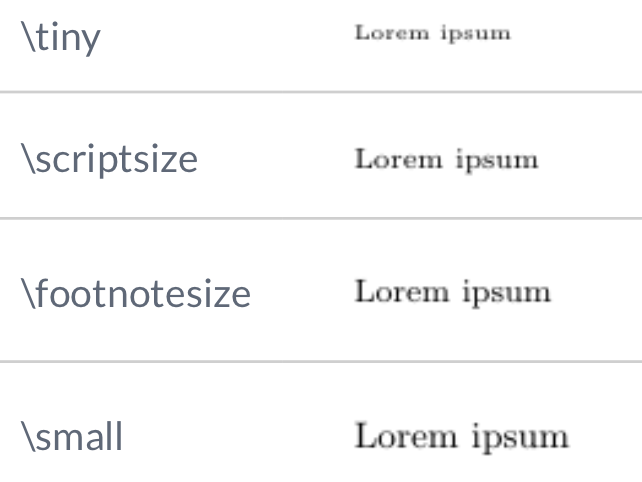
\includegraphics[width=0.5\linewidth]{figures/sample-content/latex_font_sizes} 

}

\caption{Font sizes in LaTeX}\label{fig:latex-font-sizing}
\end{figure}

You could use these to manually adjust the font size in your longtable in two steps:

\begin{enumerate}
\def\labelenumi{\arabic{enumi}.}
\tightlist
\item
  Wrap the longtable environment in, e.g., a \texttt{scriptsize} environment, by doing a string replacement in the output from \texttt{kable}/\texttt{kableExtra}
\item
  Add the attributes that make R Markdown understand that the table is a table (it seems R drops these when we do the string replacement)
\end{enumerate}

\begin{Shaded}
\begin{Highlighting}[]
\NormalTok{our\_adjusted\_table \textless{}{-}}\StringTok{ }\NormalTok{a\_long\_table }\OperatorTok{\%\textgreater{}\%}\StringTok{ }
\StringTok{  }\KeywordTok{kable}\NormalTok{(}\DataTypeTok{booktabs =} \OtherTok{TRUE}\NormalTok{, }\DataTypeTok{longtable =} \OtherTok{TRUE}\NormalTok{) }\OperatorTok{\%\textgreater{}\%}\StringTok{ }
\StringTok{  }\KeywordTok{kable\_styling}\NormalTok{(}\DataTypeTok{latex\_options =} \StringTok{"repeat\_header"}\NormalTok{) }\OperatorTok{\%\textgreater{}\%}\StringTok{ }
\StringTok{  }\CommentTok{\# wrap the longtable in a tiny environment}
\StringTok{  }\KeywordTok{str\_replace}\NormalTok{(}\StringTok{\textquotesingle{}}\CharTok{\textbackslash{}\textbackslash{}\textbackslash{}\textbackslash{}}\StringTok{begin}\CharTok{\textbackslash{}\textbackslash{}}\StringTok{\{longtable}\CharTok{\textbackslash{}\textbackslash{}}\StringTok{\}\textquotesingle{}}\NormalTok{, }
              \StringTok{\textquotesingle{}}\CharTok{\textbackslash{}\textbackslash{}\textbackslash{}\textbackslash{}}\StringTok{begin}\CharTok{\textbackslash{}\textbackslash{}}\StringTok{\{scriptsize}\CharTok{\textbackslash{}\textbackslash{}}\StringTok{\}}\CharTok{\textbackslash{}n\textbackslash{}\textbackslash{}\textbackslash{}\textbackslash{}}\StringTok{begin}\CharTok{\textbackslash{}\textbackslash{}}\StringTok{\{longtable}\CharTok{\textbackslash{}\textbackslash{}}\StringTok{\}\textquotesingle{}}\NormalTok{) }\OperatorTok{\%\textgreater{}\%}
\StringTok{  }\KeywordTok{str\_replace}\NormalTok{(}\StringTok{\textquotesingle{}}\CharTok{\textbackslash{}\textbackslash{}\textbackslash{}\textbackslash{}}\StringTok{end}\CharTok{\textbackslash{}\textbackslash{}}\StringTok{\{longtable}\CharTok{\textbackslash{}\textbackslash{}}\StringTok{\}\textquotesingle{}}\NormalTok{, }
              \StringTok{\textquotesingle{}}\CharTok{\textbackslash{}\textbackslash{}\textbackslash{}\textbackslash{}}\StringTok{end}\CharTok{\textbackslash{}\textbackslash{}}\StringTok{\{longtable}\CharTok{\textbackslash{}\textbackslash{}}\StringTok{\}}\CharTok{\textbackslash{}n\textbackslash{}\textbackslash{}\textbackslash{}\textbackslash{}}\StringTok{end}\CharTok{\textbackslash{}\textbackslash{}}\StringTok{\{scriptsize}\CharTok{\textbackslash{}\textbackslash{}}\StringTok{\}\textquotesingle{}}\NormalTok{)}

\CommentTok{\#add attributes to make R Markdown treat this as a kable LaTeX table again}
\NormalTok{our\_adjusted\_table }\OperatorTok{\%\textgreater{}\%}\StringTok{ }
\StringTok{  }\KeywordTok{structure}\NormalTok{(}\DataTypeTok{format =} \StringTok{"latex"}\NormalTok{, }\DataTypeTok{class =} \StringTok{"knitr\_kable"}\NormalTok{)}
\end{Highlighting}
\end{Shaded}

\begin{scriptsize}
\begin{longtable}{lrrrrrrrrrrr}
\toprule
  & mpg & cyl & disp & hp & drat & wt & qsec & vs & am & gear & carb\\
\midrule
\endfirsthead
\multicolumn{12}{@{}l}{\textit{(continued)}}\\
\toprule
  & mpg & cyl & disp & hp & drat & wt & qsec & vs & am & gear & carb\\
\midrule
\endhead

\endfoot
\bottomrule
\endlastfoot
Mazda RX4 & 21.0 & 6 & 160.0 & 110 & 3.90 & 2.620 & 16.46 & 0 & 1 & 4 & 4\\
Mazda RX4 Wag & 21.0 & 6 & 160.0 & 110 & 3.90 & 2.875 & 17.02 & 0 & 1 & 4 & 4\\
Datsun 710 & 22.8 & 4 & 108.0 & 93 & 3.85 & 2.320 & 18.61 & 1 & 1 & 4 & 1\\
Hornet 4 Drive & 21.4 & 6 & 258.0 & 110 & 3.08 & 3.215 & 19.44 & 1 & 0 & 3 & 1\\
Hornet Sportabout & 18.7 & 8 & 360.0 & 175 & 3.15 & 3.440 & 17.02 & 0 & 0 & 3 & 2\\
\addlinespace
Valiant & 18.1 & 6 & 225.0 & 105 & 2.76 & 3.460 & 20.22 & 1 & 0 & 3 & 1\\
Duster 360 & 14.3 & 8 & 360.0 & 245 & 3.21 & 3.570 & 15.84 & 0 & 0 & 3 & 4\\
Merc 240D & 24.4 & 4 & 146.7 & 62 & 3.69 & 3.190 & 20.00 & 1 & 0 & 4 & 2\\
Merc 230 & 22.8 & 4 & 140.8 & 95 & 3.92 & 3.150 & 22.90 & 1 & 0 & 4 & 2\\
Merc 280 & 19.2 & 6 & 167.6 & 123 & 3.92 & 3.440 & 18.30 & 1 & 0 & 4 & 4\\
\addlinespace
Merc 280C & 17.8 & 6 & 167.6 & 123 & 3.92 & 3.440 & 18.90 & 1 & 0 & 4 & 4\\
Merc 450SE & 16.4 & 8 & 275.8 & 180 & 3.07 & 4.070 & 17.40 & 0 & 0 & 3 & 3\\
Merc 450SL & 17.3 & 8 & 275.8 & 180 & 3.07 & 3.730 & 17.60 & 0 & 0 & 3 & 3\\
Merc 450SLC & 15.2 & 8 & 275.8 & 180 & 3.07 & 3.780 & 18.00 & 0 & 0 & 3 & 3\\
Cadillac Fleetwood & 10.4 & 8 & 472.0 & 205 & 2.93 & 5.250 & 17.98 & 0 & 0 & 3 & 4\\
\addlinespace
Lincoln Continental & 10.4 & 8 & 460.0 & 215 & 3.00 & 5.424 & 17.82 & 0 & 0 & 3 & 4\\
Chrysler Imperial & 14.7 & 8 & 440.0 & 230 & 3.23 & 5.345 & 17.42 & 0 & 0 & 3 & 4\\
Fiat 128 & 32.4 & 4 & 78.7 & 66 & 4.08 & 2.200 & 19.47 & 1 & 1 & 4 & 1\\
Honda Civic & 30.4 & 4 & 75.7 & 52 & 4.93 & 1.615 & 18.52 & 1 & 1 & 4 & 2\\
Toyota Corolla & 33.9 & 4 & 71.1 & 65 & 4.22 & 1.835 & 19.90 & 1 & 1 & 4 & 1\\
\addlinespace
Toyota Corona & 21.5 & 4 & 120.1 & 97 & 3.70 & 2.465 & 20.01 & 1 & 0 & 3 & 1\\
Dodge Challenger & 15.5 & 8 & 318.0 & 150 & 2.76 & 3.520 & 16.87 & 0 & 0 & 3 & 2\\
AMC Javelin & 15.2 & 8 & 304.0 & 150 & 3.15 & 3.435 & 17.30 & 0 & 0 & 3 & 2\\
Camaro Z28 & 13.3 & 8 & 350.0 & 245 & 3.73 & 3.840 & 15.41 & 0 & 0 & 3 & 4\\
Pontiac Firebird & 19.2 & 8 & 400.0 & 175 & 3.08 & 3.845 & 17.05 & 0 & 0 & 3 & 2\\
\addlinespace
Fiat X1-9 & 27.3 & 4 & 79.0 & 66 & 4.08 & 1.935 & 18.90 & 1 & 1 & 4 & 1\\
Porsche 914-2 & 26.0 & 4 & 120.3 & 91 & 4.43 & 2.140 & 16.70 & 0 & 1 & 5 & 2\\
Lotus Europa & 30.4 & 4 & 95.1 & 113 & 3.77 & 1.513 & 16.90 & 1 & 1 & 5 & 2\\
Ford Pantera L & 15.8 & 8 & 351.0 & 264 & 4.22 & 3.170 & 14.50 & 0 & 1 & 5 & 4\\
Ferrari Dino & 19.7 & 6 & 145.0 & 175 & 3.62 & 2.770 & 15.50 & 0 & 1 & 5 & 6\\
\addlinespace
Maserati Bora & 15.0 & 8 & 301.0 & 335 & 3.54 & 3.570 & 14.60 & 0 & 1 & 5 & 8\\
Volvo 142E & 21.4 & 4 & 121.0 & 109 & 4.11 & 2.780 & 18.60 & 1 & 1 & 4 & 2\\
Mazda RX41 & 21.0 & 6 & 160.0 & 110 & 3.90 & 2.620 & 16.46 & 0 & 1 & 4 & 4\\
Mazda RX4 Wag1 & 21.0 & 6 & 160.0 & 110 & 3.90 & 2.875 & 17.02 & 0 & 1 & 4 & 4\\
Datsun 7101 & 22.8 & 4 & 108.0 & 93 & 3.85 & 2.320 & 18.61 & 1 & 1 & 4 & 1\\
\addlinespace
Hornet 4 Drive1 & 21.4 & 6 & 258.0 & 110 & 3.08 & 3.215 & 19.44 & 1 & 0 & 3 & 1\\
Hornet Sportabout1 & 18.7 & 8 & 360.0 & 175 & 3.15 & 3.440 & 17.02 & 0 & 0 & 3 & 2\\
Valiant1 & 18.1 & 6 & 225.0 & 105 & 2.76 & 3.460 & 20.22 & 1 & 0 & 3 & 1\\
Duster 3601 & 14.3 & 8 & 360.0 & 245 & 3.21 & 3.570 & 15.84 & 0 & 0 & 3 & 4\\
Merc 240D1 & 24.4 & 4 & 146.7 & 62 & 3.69 & 3.190 & 20.00 & 1 & 0 & 4 & 2\\
\addlinespace
Merc 2301 & 22.8 & 4 & 140.8 & 95 & 3.92 & 3.150 & 22.90 & 1 & 0 & 4 & 2\\
Merc 2801 & 19.2 & 6 & 167.6 & 123 & 3.92 & 3.440 & 18.30 & 1 & 0 & 4 & 4\\
Merc 280C1 & 17.8 & 6 & 167.6 & 123 & 3.92 & 3.440 & 18.90 & 1 & 0 & 4 & 4\\
Merc 450SE1 & 16.4 & 8 & 275.8 & 180 & 3.07 & 4.070 & 17.40 & 0 & 0 & 3 & 3\\
Merc 450SL1 & 17.3 & 8 & 275.8 & 180 & 3.07 & 3.730 & 17.60 & 0 & 0 & 3 & 3\\
\addlinespace
Merc 450SLC1 & 15.2 & 8 & 275.8 & 180 & 3.07 & 3.780 & 18.00 & 0 & 0 & 3 & 3\\
Cadillac Fleetwood1 & 10.4 & 8 & 472.0 & 205 & 2.93 & 5.250 & 17.98 & 0 & 0 & 3 & 4\\
Lincoln Continental1 & 10.4 & 8 & 460.0 & 215 & 3.00 & 5.424 & 17.82 & 0 & 0 & 3 & 4\\
Chrysler Imperial1 & 14.7 & 8 & 440.0 & 230 & 3.23 & 5.345 & 17.42 & 0 & 0 & 3 & 4\\
Fiat 1281 & 32.4 & 4 & 78.7 & 66 & 4.08 & 2.200 & 19.47 & 1 & 1 & 4 & 1\\
\addlinespace
Honda Civic1 & 30.4 & 4 & 75.7 & 52 & 4.93 & 1.615 & 18.52 & 1 & 1 & 4 & 2\\
Toyota Corolla1 & 33.9 & 4 & 71.1 & 65 & 4.22 & 1.835 & 19.90 & 1 & 1 & 4 & 1\\
Toyota Corona1 & 21.5 & 4 & 120.1 & 97 & 3.70 & 2.465 & 20.01 & 1 & 0 & 3 & 1\\
Dodge Challenger1 & 15.5 & 8 & 318.0 & 150 & 2.76 & 3.520 & 16.87 & 0 & 0 & 3 & 2\\
AMC Javelin1 & 15.2 & 8 & 304.0 & 150 & 3.15 & 3.435 & 17.30 & 0 & 0 & 3 & 2\\
\addlinespace
Camaro Z281 & 13.3 & 8 & 350.0 & 245 & 3.73 & 3.840 & 15.41 & 0 & 0 & 3 & 4\\
Pontiac Firebird1 & 19.2 & 8 & 400.0 & 175 & 3.08 & 3.845 & 17.05 & 0 & 0 & 3 & 2\\
Fiat X1-91 & 27.3 & 4 & 79.0 & 66 & 4.08 & 1.935 & 18.90 & 1 & 1 & 4 & 1\\
Porsche 914-21 & 26.0 & 4 & 120.3 & 91 & 4.43 & 2.140 & 16.70 & 0 & 1 & 5 & 2\\
Lotus Europa1 & 30.4 & 4 & 95.1 & 113 & 3.77 & 1.513 & 16.90 & 1 & 1 & 5 & 2\\
\addlinespace
Ford Pantera L1 & 15.8 & 8 & 351.0 & 264 & 4.22 & 3.170 & 14.50 & 0 & 1 & 5 & 4\\
Ferrari Dino1 & 19.7 & 6 & 145.0 & 175 & 3.62 & 2.770 & 15.50 & 0 & 1 & 5 & 6\\
Maserati Bora1 & 15.0 & 8 & 301.0 & 335 & 3.54 & 3.570 & 14.60 & 0 & 1 & 5 & 8\\
Volvo 142E1 & 21.4 & 4 & 121.0 & 109 & 4.11 & 2.780 & 18.60 & 1 & 1 & 4 & 2\\*
\end{longtable}
\end{scriptsize}

\hypertarget{customisations-and-extensions}{%
\chapter{Customisations and extensions}\label{customisations-and-extensions}}

\minitoc 

\noindent This chapter describes a number of additional tips and tricks as well as possible customizations to the \texttt{oxforddown} thesis.

\hypertarget{front-matter}{%
\section{Front matter}\label{front-matter}}

\hypertarget{shorten-captions-shown-in-the-list-of-figures-pdf}{%
\subsection{Shorten captions shown in the list of figures (PDF)}\label{shorten-captions-shown-in-the-list-of-figures-pdf}}

You might want your list of figures (which follows the table of contents) to have shorter (or just different) figure descriptions than the actual figure captions.

Do this using the chunk option \texttt{fig.scap} (`short caption'), for example \texttt{\{r\ captain-image,\ fig.cap="A\ very\ long\ and\ descriptive\ (and\ potentially\ boring)\ caption\ that\ doesn\textquotesingle{}t\ fit\ in\ the\ list\ of\ figures,\ but\ helps\ the\ reader\ understand\ what\ the\ figure\ communicates.",\ fig.scap="A\ concise\ description\ for\ the\ list\ of\ figures"}

\hypertarget{shorten-captions-shown-in-the-list-of-tables-pdf}{%
\subsection{Shorten captions shown in the list of tables (PDF)}\label{shorten-captions-shown-in-the-list-of-tables-pdf}}

You might want your list of tables (which follows the list of figures in your thesis front matter) to have shorter (or just different) table descriptions than the actual table captions.

If you are using \texttt{knitr::kable} to generate a table, you can do this with the argument \texttt{caption.short}, e.g.:

\begin{Shaded}
\begin{Highlighting}[]
\NormalTok{knitr}\OperatorTok{::}\KeywordTok{kable}\NormalTok{(mtcars,}
              \DataTypeTok{caption =} \StringTok{"A very long and descriptive (and potentially}
\StringTok{              boring) caption that doesn\textquotesingle{}t fit in the list of figures,}
\StringTok{              but helps the reader understand what the figure }
\StringTok{              communicates."}\NormalTok{,}
              \DataTypeTok{caption.short =} \StringTok{"A concise description for the list of tables"}\NormalTok{)}
\end{Highlighting}
\end{Shaded}

\hypertarget{shorten-running-header-pdf}{%
\section{Shorten running header (PDF)}\label{shorten-running-header-pdf}}

You might want a chapter's running header (i.e.~the header showing the title of the current chapter at the top of page) to be shorter (or just different) to the actual chapter title.

Do this by adding the latex command \texttt{\textbackslash{}chaptermark\{My\ shorter\ version\}} after your chapter title.

For example, chapter \ref{cites-and-refs}`s running header is simply 'Cites and cross-refs', because it begins like this:

\begin{Shaded}
\begin{Highlighting}[]
\FunctionTok{\# Citations, cross{-}references, and collaboration \{\#cites{-}and{-}refs\} }
\NormalTok{\textbackslash{}chaptermark\{Cites and cross{-}refs\}}
\end{Highlighting}
\end{Shaded}

\hypertarget{unnumbered-chapters}{%
\section{Unnumbered chapters}\label{unnumbered-chapters}}

To make chapters unnumbered (normally only relevant to the Introduction and/or the Conclusion), follow the chapter header with \texttt{\{-\}}, e.g.~\texttt{\#\ Introduction\ \{-\}}.

When you do this, you must also follow the heading with these two latex commands:

\begin{Shaded}
\begin{Highlighting}[]
\FunctionTok{\textbackslash{}adjustmtc}
\FunctionTok{\textbackslash{}markboth}\NormalTok{\{The Name of Your Unnumbered Chapter\}\{\}}
\end{Highlighting}
\end{Shaded}

Otherwise the chapter's mini table of contents and the running header will show the previous chapter.

\hypertarget{beginning-chapters-with-quotes-pdf}{%
\section{Beginning chapters with quotes (PDF)}\label{beginning-chapters-with-quotes-pdf}}

The OxThesis LaTeX template lets you inject some wittiness into your thesis by including a block of type \texttt{savequote} at the beginning of chapters.
To do this, use the syntax \texttt{\textasciigrave{}\textasciigrave{}\textasciigrave{}\{block\ type=\textquotesingle{}savequote\textquotesingle{}\}}.\footnote{For more on custom block types, see the relevant section in \href{https://bookdown.org/yihui/bookdown/custom-blocks.html}{\emph{Authoring Books with R Markdown}}.}

Add the reference for the quote with the chunk option \texttt{quote\_author="my\ author\ name"}.
You will also want to add the chunk option \texttt{include=knitr::is\_latex\_output()} so that quotes are only included in PDF output.

It's not possible to use markdown syntax inside chunk options, so if you want to e.g.~italicise a book name in the reference use a \href{https://bookdown.org/yihui/bookdown/markdown-extensions-by-bookdown.html\#text-references}{`text reference'}: Create a named piece of text with `(ref:label-name) My text', then point to this in the chunk option with \texttt{quote\_author=\textquotesingle{}(ref:label-name)\textquotesingle{}}.

\hypertarget{highlighting-corrections-html-pdf}{%
\section{Highlighting corrections (HTML \& PDF)}\label{highlighting-corrections-html-pdf}}

For when it comes time to do corrections, you may want to highlight changes made when you submit a post-viva, corrected copy to your examiners so they can quickly verify you've completed the task.
You can do so like this:

\hypertarget{short-inline-corrections}{%
\subsection{Short, inline corrections}\label{short-inline-corrections}}

Highlight \textbf{short, inline corrections} by doing \texttt{{[}like\ this{]}\{.correction\}} --- the text between the square brackets will then \hl{be highlighted in blue} in the output.

Note that pandoc might get confused by citations and cross-references inside inline corrections.
In particular, it might get confused by \texttt{"{[}what\ @Shea2014\ said{]}\{.correction\}"} which becomes \autocite[what][ said]{Shea2014}\{.correction\}
In such cases, you can use LaTeX syntax directly.
The correction highlighting uses the \href{https://ctan.org/pkg/soul}{soul} package, so you can do like this:

\begin{itemize}
\tightlist
\item
  If using biblatex for references, use \texttt{"\textbackslash{}hl\{what\ \textbackslash{}textcite\{Shea2014\}\ said\}}
\item
  If using natbib for references, use \texttt{"\textbackslash{}hl\{what\ \textbackslash{}cite\{Shea2014\}\ said\}}
\end{itemize}

Using raw LaTeX has the drawback of corrections then not showing up in HTML output at all, but you might only care about correction highlighting in the PDF for your examiners anyway!

\hypertarget{blocks-of-added-or-changed-material}{%
\subsection{Blocks of added or changed material}\label{blocks-of-added-or-changed-material}}

Highlight entire \textbf{blocks of added or changed material} by putting them in a block of type \texttt{correction}, using the syntax \texttt{\textasciigrave{}\textasciigrave{}\textasciigrave{}\{block\ type=\textquotesingle{}correction\textquotesingle{}\}}.\footnote{In the \textbf{.tex} file for PDF output, this will put the content between \texttt{\textbackslash{}begin\{correction\}} and \texttt{\textbackslash{}end\{correction\}}; in gitbook output it will be put between \texttt{\textless{}div\ class="correction"\textgreater{}} and \texttt{\textless{}/div\textgreater{}}.}
Like so:

\begin{correction}
For larger chunks, like this paragraph or indeed entire figures, you can
use the \texttt{correction} block type. This environment
\textbf{highlights paragraph-sized and larger blocks} with the same blue
colour.
\end{correction}

\emph{Note that correction blocks cannot be included in word output.}

\hypertarget{stopping-corrections-from-being-highlighted}{%
\subsection{Stopping corrections from being highlighted}\label{stopping-corrections-from-being-highlighted}}

To turn off correction highlighting, go to the YAML header of \textbf{index.Rmd}, then:

\begin{itemize}
\tightlist
\item
  PDF output: set \texttt{corrections:\ false}\\
\item
  HTML output: remove or comment out \texttt{-\ templates/corrections.css}
\end{itemize}

\hypertarget{apply-custom-font-color-and-highlighting-to-text-html-pdf}{%
\section{Apply custom font color and highlighting to text (HTML \& PDF)}\label{apply-custom-font-color-and-highlighting-to-text-html-pdf}}

The lua filter that adds the functionality to highlight corrections adds two more tricks:
you can apply your own choice of colour to highlight text, or change the font color.
The syntax is as follows:

\begin{quote}
Here's \texttt{{[}some\ text\ in\ pink\ highlighting{]}\{highlight="pink"\}}\\
Becomes: Here's \sethlcolor{pink}\hl{some text in pink highlighting}\sethlcolor{correctioncolor}.
\end{quote}

\begin{quote}
\texttt{{[}Here\textquotesingle{}s\ some\ text\ with\ blue\ font{]}\{color="blue"\}}~\\
Becomes: \textcolor{blue}{Here's some text with blue font}
\end{quote}

\begin{quote}
Finally --- never, ever actually do this -- \texttt{{[}here\textquotesingle{}s\ some\ text\ with\ black\ highlighting\ and\ yellow\ font{]}\{highlight="black"\ color="yellow"\}}\\
Becomes: \textcolor{yellow}{\sethlcolor{black}\hl{here's some text with black highlighting and yellow font}\sethlcolor{correctioncolor}}
\end{quote}

The file \textbf{scripts\_and\_filters/colour\_and\_highlight.lua} implements this, if you want to fiddle around with it.
It works with both PDF and HTML output.

\hypertarget{embed-pdf}{%
\section{Including another paper in your thesis - embed a PDF document}\label{embed-pdf}}

You may want to embed existing PDF documents into the thesis, for example if your department allows a `portfolio' style thesis and you need to include an existing typeset publication as a chapter.

In gitbook output, you can simply use \texttt{knitr::include\_graphics} and it should include a scrollable (and downloadable) PDF.
You will probably want to set the chunk options \texttt{out.width=\textquotesingle{}100\%\textquotesingle{}} and \texttt{out.height=\textquotesingle{}1000px\textquotesingle{}}:

\begin{Shaded}
\begin{Highlighting}[]
\NormalTok{knitr}\OperatorTok{::}\KeywordTok{include\_graphics}\NormalTok{(}\StringTok{"figures/sample{-}content/pdf\_embed\_example/Lyngs2020\_FB.pdf"}\NormalTok{)}
\end{Highlighting}
\end{Shaded}

In LaTeX output, however, this approach can cause odd behaviour.
Therefore, when you build your thesis to PDF, split the PDF into an alphanumerically sorted sequence of \textbf{single-page} PDF files (you can do this automatically with the package \texttt{pdftools}). You can then use the appropriate LaTeX command to insert them, as shown below (for brevity, in the \texttt{oxforddown} PDF sample content we're only including two pages).
\emph{Note that the chunk option \texttt{results=\textquotesingle{}asis\textquotesingle{}} must be set.}
You may also want to remove margins from the PDF files, which you can do with Adobe Acrobat (paid version) and likely other software.

\begin{Shaded}
\begin{Highlighting}[]
\CommentTok{\# install.packages(pdftools)}
\CommentTok{\# split PDF into pages stored in}
\NormalTok{    figures}\OperatorTok{/}\NormalTok{sample}\OperatorTok{{-}}\NormalTok{content}\OperatorTok{/}\NormalTok{pdf\_embed\_example}\OperatorTok{/}\NormalTok{split}\OperatorTok{/}
\CommentTok{\#}
\StringTok{    }\NormalTok{pdftools}\OperatorTok{::}\KeywordTok{pdf\_split}\NormalTok{(}\StringTok{"figures/sample{-}content/pdf\_embed\_example/Lyngs2020\_FB.pdf"}\NormalTok{,}
\CommentTok{\# output = "figures/sample{-}content/pdf\_embed\_example/split/")}

\CommentTok{\# grab the pages}
\NormalTok{pages \textless{}{-}}\StringTok{ }\KeywordTok{list.files}\NormalTok{(}\StringTok{"figures/sample{-}content/pdf\_embed\_example/split"}\NormalTok{,}
    \DataTypeTok{full.names =} \OtherTok{TRUE}\NormalTok{)}

\CommentTok{\# set how wide you want the inserted PDFs to be:}
\CommentTok{\# 1.0 is 100 per cent of the oxforddown PDF page width;}
\CommentTok{\# you may want to make it a bit bigger}
\NormalTok{pdf\_width \textless{}{-}}\StringTok{ }\FloatTok{1.2}

\CommentTok{\# for each PDF page, insert it nicely and}
\CommentTok{\# end with a page break}
\KeywordTok{cat}\NormalTok{(stringr}\OperatorTok{::}\KeywordTok{str\_c}\NormalTok{(}\StringTok{"}\CharTok{\textbackslash{}\textbackslash{}}\StringTok{newpage }\CharTok{\textbackslash{}\textbackslash{}}\StringTok{begin\{center\}}
\StringTok{    }\CharTok{\textbackslash{}\textbackslash{}}\StringTok{makebox[}\CharTok{\textbackslash{}\textbackslash{}}\StringTok{linewidth][c]\{}\CharTok{\textbackslash{}\textbackslash{}}\StringTok{includegraphics[width="}\NormalTok{, pdf\_width,}
    \StringTok{"}\CharTok{\textbackslash{}\textbackslash{}}\StringTok{linewidth]\{"}\NormalTok{, pages, }\StringTok{"\}\} }\CharTok{\textbackslash{}\textbackslash{}}\StringTok{end\{center\}"}\NormalTok{))}
\end{Highlighting}
\end{Shaded}

\newpage \begin{center} \makebox[\linewidth][c]{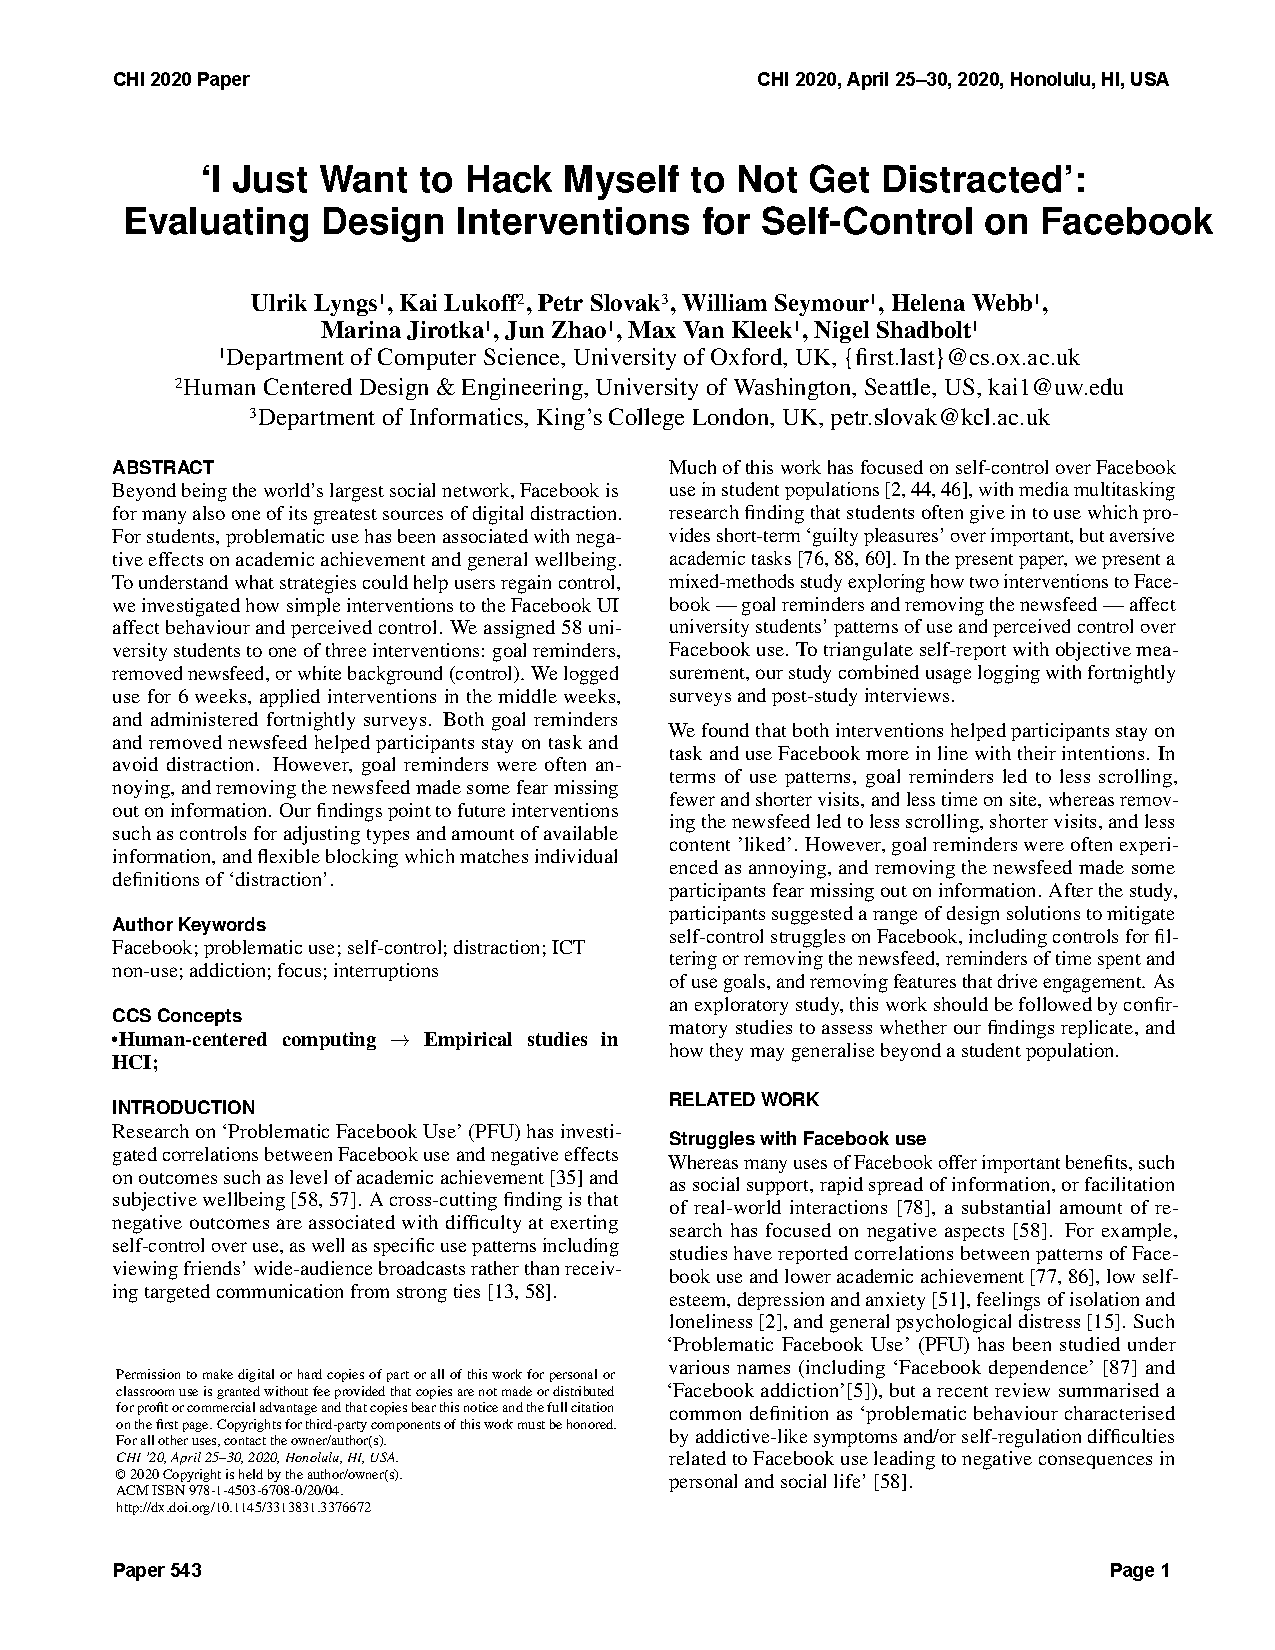
\includegraphics[width=1.2\linewidth]{figures/sample-content/pdf_embed_example/split/_000000000000001.pdf}} \end{center} \newpage \begin{center} \makebox[\linewidth][c]{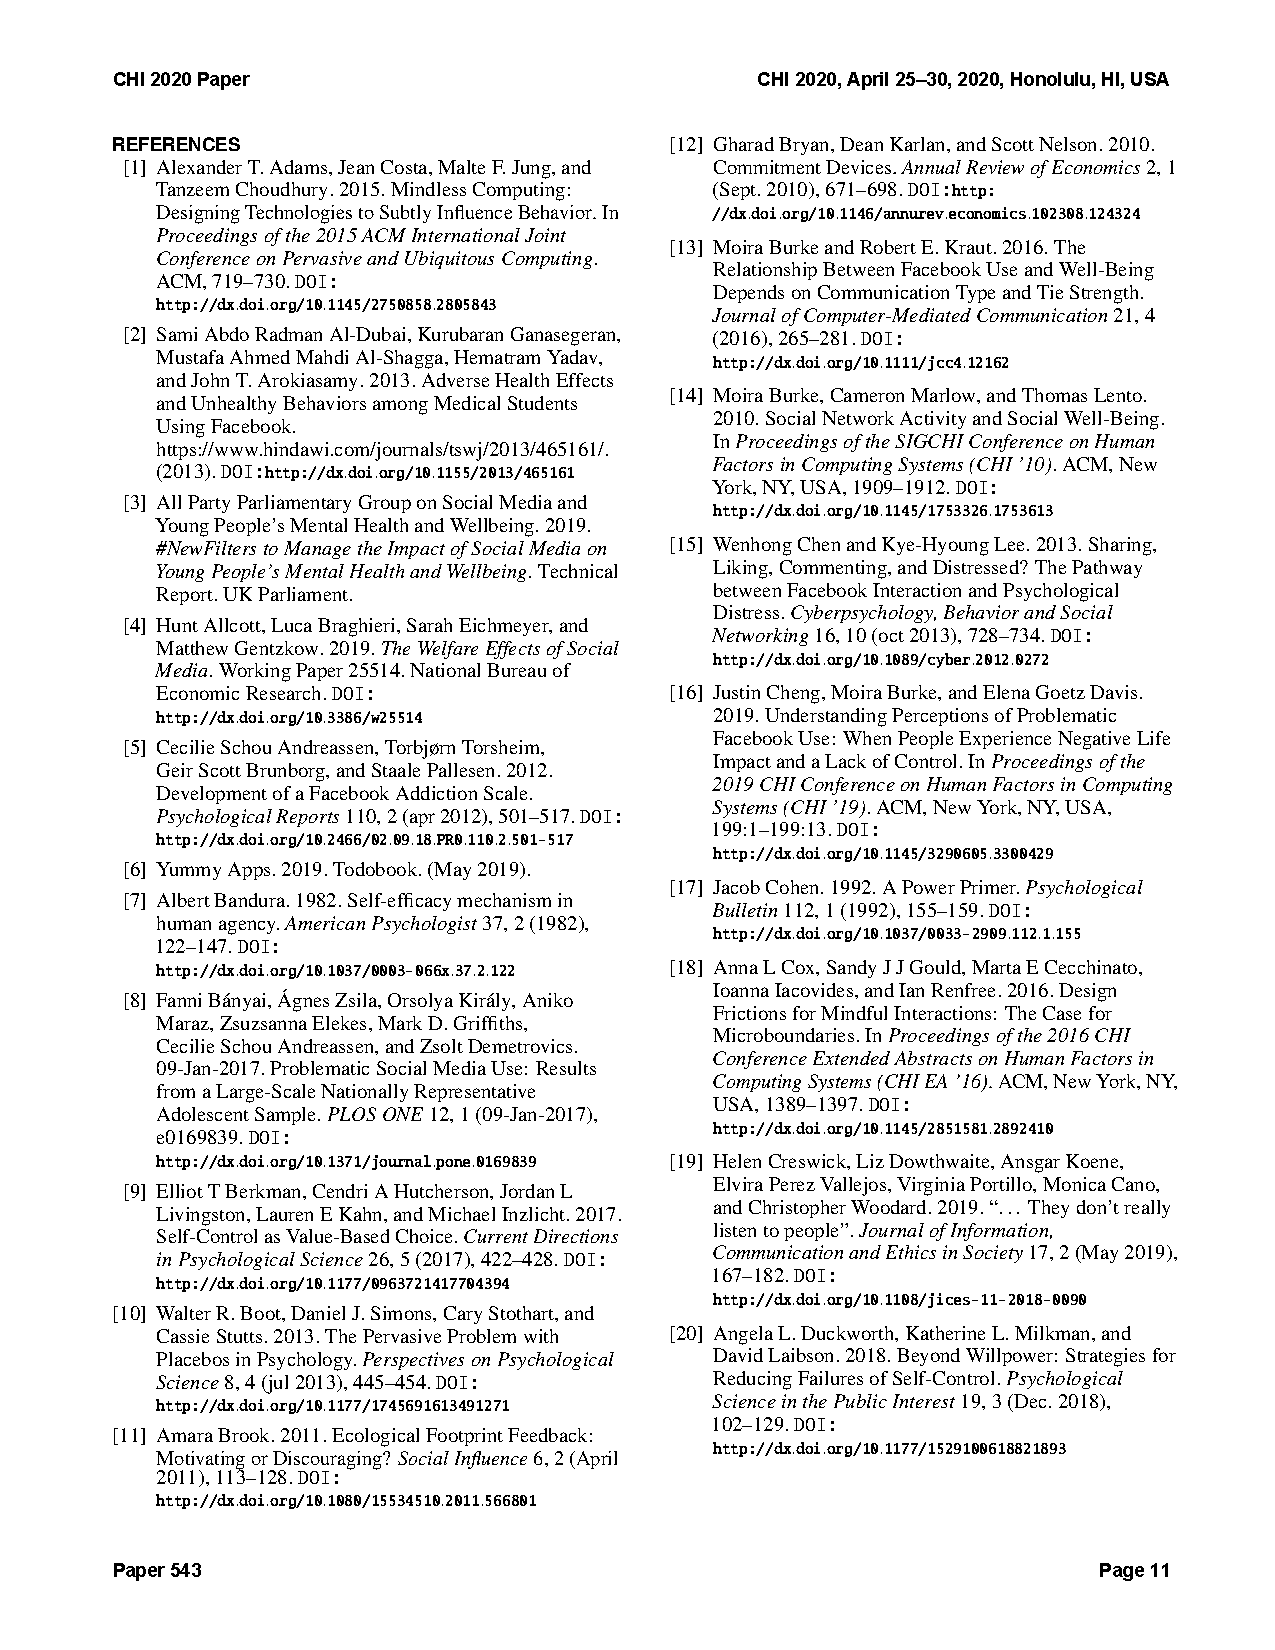
\includegraphics[width=1.2\linewidth]{figures/sample-content/pdf_embed_example/split/_000000000000011.pdf}} \end{center}

\hypertarget{embed-rmd}{%
\section{Including another paper in your thesis - R Markdown child document}\label{embed-rmd}}

Sometimes you want to include another paper you are currently writing as a chapter in your thesis.
Above \ref{embed-pdf}, we described the simplest way to do this: include the other paper as a pdf.
However, in some cases you instead want to include the R Markdown source from this paper, and have it compiled within your thesis.
This is a little bit more tricky, because you need to keep careful track of your file paths, but it is possible by \href{https://bookdown.org/yihui/rmarkdown-cookbook/child-document.html}{including the paper as a child document}.
There are four main steps:

\begin{enumerate}
\def\labelenumi{\arabic{enumi}.}
\tightlist
\item
  Include the paper as a child document
\item
  Make file paths compatible with knitting the article on its own, as well as when it's include in your thesis
\item
  Make header levels correct
\item
  Make figure widths correct
\end{enumerate}

\hypertarget{an-example-paper-in-another-folder}{%
\subsection{An example paper in another folder}\label{an-example-paper-in-another-folder}}

Take this simple example (files for this are in \href{https://github.com/ulyngs/oxforddown-external-article}{this GitHub repository}):

\begin{Shaded}
\begin{Highlighting}[]
\NormalTok{|{-}{-}paper\_to\_include}
\NormalTok{|  |{-}{-}my\_paper.Rmd}
\NormalTok{|  |{-}{-}data}
\NormalTok{|  |  |{-}{-}cat\_salt.csv}
\NormalTok{|  |{-}{-}figures}
\NormalTok{|  |  |{-}{-}cat.jpg}
\NormalTok{|}
\NormalTok{|{-}{-}thesis}
\end{Highlighting}
\end{Shaded}

As the chart suggests, you have another folder, \textbf{paper\_to\_include/} living in the same containing folder as your thesis folder.
In the \textbf{paper\_to\_include} folder, the file \textbf{my\_paper.Rmd} is where you write the paper.
In \textbf{my\_paper.Rmd}, you read in a CSV file found in the subfolder \textbf{data/cats.csv}, and also an image from the subfolder \textbf{figures/cat.jpg}.

\hypertarget{step-1-include-paper-as-a-child-document}{%
\subsection{Step 1: Include paper as a child document}\label{step-1-include-paper-as-a-child-document}}

In your thesis folder, create an Rmd file for the chapter where you want to include another paper.
Add one or more code chunks that include R Markdown files from that paper as child documents:

\begin{Shaded}
\begin{Highlighting}[]
\FunctionTok{\# Including an external chapter }

\InformationTok{\textasciigrave{}\textasciigrave{}\textasciigrave{}\{r child = "../paper\_to\_include/my\_paper.Rmd"\}}
\InformationTok{\textasciigrave{}\textasciigrave{}\textasciigrave{}}
\end{Highlighting}
\end{Shaded}

\hypertarget{step-2-make-file-paths-compatible}{%
\subsection{Step 2: Make file paths compatible}\label{step-2-make-file-paths-compatible}}

Use \href{https://rmarkdown.rstudio.com/lesson-6.html}{parameters} to adjust the file path of images based on values you set in the YAML header of an R Markdown file.
In \textbf{my\_paper.Rmd}, create a parameter called \texttt{other\_path} and set it to an empty string:

\begin{Shaded}
\begin{Highlighting}[]
\PreprocessorTok{{-}{-}{-}}
\FunctionTok{title}\KeywordTok{:}\AttributeTok{ }\StringTok{"A fabulous article in a different folder"}
\FunctionTok{params}\KeywordTok{:}
\AttributeTok{  }\FunctionTok{other\_path}\KeywordTok{:}\AttributeTok{ }\StringTok{""}
\PreprocessorTok{{-}{-}{-}}
\end{Highlighting}
\end{Shaded}

In \textbf{my\_paper.Rmd}, put this at the start of the filepath when you read in data or include images:

\begin{Shaded}
\begin{Highlighting}[]
\KeywordTok{library}\NormalTok{(tidyverse)}
\KeywordTok{library}\NormalTok{(knitr)}

\NormalTok{cat\_data \textless{}{-}}\StringTok{ }\KeywordTok{read\_csv}\NormalTok{(}\KeywordTok{str\_c}\NormalTok{(params}\OperatorTok{$}\NormalTok{other\_path, }\StringTok{"data/cats.csv"}\NormalTok{))}
\KeywordTok{include\_graphics}\NormalTok{(}\KeywordTok{str\_c}\NormalTok{(params}\OperatorTok{$}\NormalTok{other\_path, }\StringTok{"figures/cat.jpg"}\NormalTok{))}
\end{Highlighting}
\end{Shaded}

Finally, in your thesis folder's \textbf{index.Rmd} file, also create the parameter \texttt{other\_path}.
But here, set it to where the \textbf{paper\_to\_include/} folder is relative to your thesis folder:

\begin{Shaded}
\begin{Highlighting}[]
\FunctionTok{params}\KeywordTok{:}
\AttributeTok{  }\FunctionTok{other\_path}\KeywordTok{:}\AttributeTok{ }\StringTok{"../paper\_to\_include/"}
\end{Highlighting}
\end{Shaded}

\hypertarget{note-on-html-output}{%
\subsubsection{Note on HTML output}\label{note-on-html-output}}

Note that if you want to host an HTML version on your thesis online, you will need to include graphics in the content that you host online - the internet obviously won't be able to see filepaths that are just referring to stuff in another folder on your computer!

\hypertarget{step-3-make-sure-header-levels-are-correct}{%
\subsection{Step 3: Make sure header levels are correct}\label{step-3-make-sure-header-levels-are-correct}}

Unless the paper you want to include is also written as a book, your header levels are probably going to be off.
That is, the level 1 headers (\# Some header) you use for main sections in the other paper turns into chaper titles when included in your thesis.

To avoid this, first \emph{increment all heading levels by one in \textbf{paper\_to\_include/my\_paper.Rmd}} (\# Some header -\textgreater{} \#\# Some header).
Then in \textbf{paper\_to\_include/} create a \href{https://bookdown.org/yihui/rmarkdown-cookbook/lua-filters.html\#lua-filters}{lua filter} that decrements header levels by one: Create a text file, save it as \textbf{reduce\_header\_level.lua}, and give it the content below.

\begin{Shaded}
\begin{Highlighting}[]
\KeywordTok{function}\NormalTok{ Header}\OperatorTok{(}\NormalTok{el}\OperatorTok{)}
  \ControlFlowTok{if} \OperatorTok{(}\NormalTok{el}\OperatorTok{.}\NormalTok{level }\OperatorTok{\textless{}=} \DecValTok{1}\OperatorTok{)} \ControlFlowTok{then}
    \FunctionTok{error}\OperatorTok{(}\StringTok{"I don\textquotesingle{}t know how to decrease the level of h1"}\OperatorTok{)}
  \ControlFlowTok{end}
\NormalTok{  el}\OperatorTok{.}\NormalTok{level }\OperatorTok{=}\NormalTok{ el}\OperatorTok{.}\NormalTok{level }\OperatorTok{{-}} \DecValTok{1}
  \ControlFlowTok{return}\NormalTok{ el}
\KeywordTok{end}
\end{Highlighting}
\end{Shaded}

In the YAML header of \textbf{paper\_to\_include/my\_paper.Rmd}, use this filter:

\begin{Shaded}
\begin{Highlighting}[]
\PreprocessorTok{{-}{-}{-}}
\FunctionTok{title}\KeywordTok{:}\AttributeTok{ }\StringTok{"A fabulous article in a different folder"}
\FunctionTok{params}\KeywordTok{:}
\AttributeTok{  }\FunctionTok{other\_path}\KeywordTok{:}\AttributeTok{ }\StringTok{""}
\FunctionTok{output}\KeywordTok{:}
\AttributeTok{  }\FunctionTok{pdf\_document}\KeywordTok{:}\AttributeTok{ }
\AttributeTok{    }\FunctionTok{pandoc\_args}\KeywordTok{:}\AttributeTok{ }\KeywordTok{[}\StringTok{"{-}{-}lua{-}filter=reduce\_header\_level.lua"}\KeywordTok{]}
\PreprocessorTok{{-}{-}{-}}
\end{Highlighting}
\end{Shaded}

Now, your header levels will be correct both when you knit the paper on its own and when its included in your thesis.

NOTE: There might be no need to use a lua filter to shift heading - it seems you could simply use \texttt{pandoc\_args:\ {[}"-\/-shift-heading-level-by=-1"{]}} (see \url{https://pandoc.org/MANUAL.html\#reader-options})

\hypertarget{step-4.-make-sure-figure-widths-are-correct}{%
\subsection{Step 4. Make sure figure widths are correct}\label{step-4.-make-sure-figure-widths-are-correct}}

It might be that your figure widths when knitting your paper on its own, and when including it in your thesis, need to be different.
You can again use parameters to set figure widths.

Imagine you want figure width to be 80\% of the page width when knitting your paper on its own, but 100\% in your thesis.
In \textbf{paper\_to\_include/my\_paper.Rmd}, first add a parameter we could call \texttt{out\_width} and set it to the string ``80\%'':

\begin{Shaded}
\begin{Highlighting}[]
\PreprocessorTok{{-}{-}{-}}
\FunctionTok{title}\KeywordTok{:}\AttributeTok{ }\StringTok{"A fabulous article in a different folder"}
\FunctionTok{params}\KeywordTok{:}
\AttributeTok{  }\FunctionTok{other\_path}\KeywordTok{:}\AttributeTok{ }\StringTok{""}
\AttributeTok{  }\FunctionTok{out\_width}\KeywordTok{:}\AttributeTok{ }\StringTok{"80\%"}
\FunctionTok{output}\KeywordTok{:}
\AttributeTok{  }\FunctionTok{pdf\_document}\KeywordTok{:}\AttributeTok{ }
\AttributeTok{    }\FunctionTok{pandoc\_args}\KeywordTok{:}\AttributeTok{ }\KeywordTok{[}\StringTok{"{-}{-}lua{-}filter=reduce\_header\_level.lua"}\KeywordTok{]}
\PreprocessorTok{{-}{-}{-}}
\end{Highlighting}
\end{Shaded}

Then, make sure use that parameter to set the output width when you include figures in \textbf{paper\_to\_include/my\_paper.Rmd}:

\begin{Shaded}
\begin{Highlighting}[]
\InformationTok{\textasciigrave{}\textasciigrave{}\textasciigrave{}\{r, out.width=params$out\_width, fig.cap="A very funny cat"\}}
\InformationTok{include\_graphics(str\_c(params$other\_path, "figures/cat.jpg"))}
\InformationTok{\textasciigrave{}\textasciigrave{}\textasciigrave{}}
\end{Highlighting}
\end{Shaded}

Finally, create the parameter \texttt{out\_width} in your thesis' \textbf{index.Rmd} file:

\begin{Shaded}
\begin{Highlighting}[]
\FunctionTok{params}\KeywordTok{:}
\AttributeTok{  }\FunctionTok{other\_path}\KeywordTok{:}\AttributeTok{ }\StringTok{"../paper\_to\_include/"}
\AttributeTok{  }\FunctionTok{out\_width}\KeywordTok{:}\AttributeTok{ }\StringTok{"80\%"}
\end{Highlighting}
\end{Shaded}

Now, the output width of your figure will be 80\% when knitting your paper on its own, and 100\% when knitting it as child document of your thesis.

\hypertarget{customizing-referencing}{%
\section{Customizing referencing}\label{customizing-referencing}}

\hypertarget{using-a-.csl-file-with-pandoc-instead-of-biblatex}{%
\subsection{Using a .csl file with pandoc instead of biblatex}\label{using-a-.csl-file-with-pandoc-instead-of-biblatex}}

The \texttt{oxforddown} package uses biblatex in LaTeX for referencing.
It is also possible to use pandoc for referencing by providing a .csl file in the YAML header of \textbf{index.Rmd} (likely requiring commenting out the biblatex code in \textbf{templates/template.tex}).
This may be helpful for those who have a .csl file describing the referencing format for a particular journal.
However, note that this approach does not support chapter bibliographies (see Section \ref{biblatex-custom}).

\begin{Shaded}
\begin{Highlighting}[]
\FunctionTok{csl}\KeywordTok{:}\AttributeTok{ ecology.csl}
\end{Highlighting}
\end{Shaded}

\hypertarget{biblatex-custom}{%
\subsection{Customizing biblatex and adding chapter bibliographies}\label{biblatex-custom}}

This section provides one example of customizing biblatex. Much of this code was combined from searches on Stack Exchange and other sources (e.g.~\href{https://tex.stackexchange.com/questions/10682/suppress-in-biblatex}{here}).

In \textbf{templates/template.tex}, one can replace the existing biblatex calls with the following to achieve referencing that looks like this:

(Charmantier and Gienapp 2014)

Charmantier, A. and P. Gienapp (2014). Climate change and timing of avian breeding and migration: evolutionary versus plastic changes. Evolutionary Applications 7(1):15--28. doi: 10.1111/eva.12126.

\begin{Shaded}
\begin{Highlighting}[]
\BuiltInTok{\textbackslash{}usepackage}\NormalTok{[backend=biber,}
\NormalTok{    bibencoding=utf8,}
\NormalTok{    refsection=chapter, }\CommentTok{\% referencing by chapter}
\NormalTok{    style=authoryear, }
\NormalTok{    firstinits=true,}
\NormalTok{    isbn=false,}
\NormalTok{    doi=true,}
\NormalTok{    url=false,}
\NormalTok{    eprint=false,}
\NormalTok{    related=false,}
\NormalTok{    dashed=false,}
\NormalTok{    clearlang=true,}
\NormalTok{    maxcitenames=2,}
\NormalTok{    mincitenames=1,}
\NormalTok{    maxbibnames=10,}
\NormalTok{    abbreviate=false,}
\NormalTok{    minbibnames=3,}
\NormalTok{    uniquelist=minyear,}
\NormalTok{    sortcites=true,}
\NormalTok{    date=year}
\NormalTok{]\{}\ExtensionTok{biblatex}\NormalTok{\}}
\FunctionTok{\textbackslash{}AtEveryBibitem}\NormalTok{\{}\CommentTok{\%}
  \FunctionTok{\textbackslash{}clearlist}\NormalTok{\{language\}}\CommentTok{\%}
  \FunctionTok{\textbackslash{}clearfield}\NormalTok{\{note\}}
\NormalTok{\}}

\FunctionTok{\textbackslash{}DeclareFieldFormat}\NormalTok{\{titlecase\}\{}\FunctionTok{\textbackslash{}MakeTitleCase}\NormalTok{\{\#1\}\}}

\FunctionTok{\textbackslash{}newrobustcmd}\NormalTok{\{}\FunctionTok{\textbackslash{}MakeTitleCase}\NormalTok{\}[1]\{}\CommentTok{\%}
  \FunctionTok{\textbackslash{}ifthenelse}\NormalTok{\{}\FunctionTok{\textbackslash{}ifcurrentfield}\NormalTok{\{booktitle\}}\FunctionTok{\textbackslash{}OR\textbackslash{}ifcurrentfield}\NormalTok{\{booksubtitle\}}\CommentTok{\%}
    \FunctionTok{\textbackslash{}OR\textbackslash{}ifcurrentfield}\NormalTok{\{maintitle\}}\FunctionTok{\textbackslash{}OR\textbackslash{}ifcurrentfield}\NormalTok{\{mainsubtitle\}}\CommentTok{\%}
    \FunctionTok{\textbackslash{}OR\textbackslash{}ifcurrentfield}\NormalTok{\{journaltitle\}}\FunctionTok{\textbackslash{}OR\textbackslash{}ifcurrentfield}\NormalTok{\{journalsubtitle\}}\CommentTok{\%}
    \FunctionTok{\textbackslash{}OR\textbackslash{}ifcurrentfield}\NormalTok{\{issuetitle\}}\FunctionTok{\textbackslash{}OR\textbackslash{}ifcurrentfield}\NormalTok{\{issuesubtitle\}}\CommentTok{\%}
    \FunctionTok{\textbackslash{}OR\textbackslash{}ifentrytype}\NormalTok{\{book\}}\FunctionTok{\textbackslash{}OR\textbackslash{}ifentrytype}\NormalTok{\{mvbook\}}\FunctionTok{\textbackslash{}OR\textbackslash{}ifentrytype}\NormalTok{\{bookinbook\}}\CommentTok{\%}
    \FunctionTok{\textbackslash{}OR\textbackslash{}ifentrytype}\NormalTok{\{booklet\}}\FunctionTok{\textbackslash{}OR\textbackslash{}ifentrytype}\NormalTok{\{suppbook\}}\CommentTok{\%}
    \FunctionTok{\textbackslash{}OR\textbackslash{}ifentrytype}\NormalTok{\{collection\}}\FunctionTok{\textbackslash{}OR\textbackslash{}ifentrytype}\NormalTok{\{mvcollection\}}\CommentTok{\%}
    \FunctionTok{\textbackslash{}OR\textbackslash{}ifentrytype}\NormalTok{\{suppcollection\}}\FunctionTok{\textbackslash{}OR\textbackslash{}ifentrytype}\NormalTok{\{manual\}}\CommentTok{\%}
    \FunctionTok{\textbackslash{}OR\textbackslash{}ifentrytype}\NormalTok{\{periodical\}}\FunctionTok{\textbackslash{}OR\textbackslash{}ifentrytype}\NormalTok{\{suppperiodical\}}\CommentTok{\%}
    \FunctionTok{\textbackslash{}OR\textbackslash{}ifentrytype}\NormalTok{\{proceedings\}}\FunctionTok{\textbackslash{}OR\textbackslash{}ifentrytype}\NormalTok{\{mvproceedings\}}\CommentTok{\%}
    \FunctionTok{\textbackslash{}OR\textbackslash{}ifentrytype}\NormalTok{\{reference\}}\FunctionTok{\textbackslash{}OR\textbackslash{}ifentrytype}\NormalTok{\{mvreference\}}\CommentTok{\%}
    \FunctionTok{\textbackslash{}OR\textbackslash{}ifentrytype}\NormalTok{\{report\}}\FunctionTok{\textbackslash{}OR\textbackslash{}ifentrytype}\NormalTok{\{thesis\}\}}
\NormalTok{    \{\#1\}}
\NormalTok{    \{}\FunctionTok{\textbackslash{}MakeSentenceCase}\NormalTok{\{\#1\}\}\}}
    
\CommentTok{\% \textbackslash{}renewbibmacro\{in:\}\{\}}
\CommentTok{\% suppress "in" for articles}
\CommentTok{\% }
\FunctionTok{\textbackslash{}renewbibmacro}\NormalTok{\{in:\}\{}\CommentTok{\%}
  \FunctionTok{\textbackslash{}ifentrytype}\NormalTok{\{article\}\{\}\{}\FunctionTok{\textbackslash{}printtext}\NormalTok{\{}\FunctionTok{\textbackslash{}bibstring}\NormalTok{\{in\}}\FunctionTok{\textbackslash{}intitlepunct}\NormalTok{\}\}\}}
\CommentTok{\%{-}{-} no "quotes" around titles of chapters/article titles}
\FunctionTok{\textbackslash{}DeclareFieldFormat}\NormalTok{[article, inbook, incollection, inproceedings, misc, thesis, unpublished]}
\NormalTok{\{title\}\{\#1\}}
\CommentTok{\%{-}{-} no punctuation after volume}
\FunctionTok{\textbackslash{}DeclareFieldFormat}\NormalTok{[article]}
\NormalTok{\{volume\}\{\{\#1\}\}}
\CommentTok{\%{-}{-} puts number/issue between brackets}
\FunctionTok{\textbackslash{}DeclareFieldFormat}\NormalTok{[article, inbook, incollection, inproceedings, misc, thesis, unpublished]}
\NormalTok{\{number\}\{}\FunctionTok{\textbackslash{}mkbibparens}\NormalTok{\{\#1\}\} }
\CommentTok{\%{-}{-} and then for articles directly the pages w/o any "pages" or "pp." }
\FunctionTok{\textbackslash{}DeclareFieldFormat}\NormalTok{[article]}
\NormalTok{\{pages\}\{\#1\}}
\CommentTok{\%{-}{-} for some types replace "pages" by "p."}
\FunctionTok{\textbackslash{}DeclareFieldFormat}\NormalTok{[inproceedings, incollection, inbook]}
\NormalTok{\{pages\}\{p. \#1\}}
\CommentTok{\%{-}{-} format 16(4):224{-}{-}225 for articles}
\FunctionTok{\textbackslash{}renewbibmacro}\NormalTok{*\{volume+number+eid\}\{}
  \FunctionTok{\textbackslash{}printfield}\NormalTok{\{volume\}}\CommentTok{\%}
  \FunctionTok{\textbackslash{}printfield}\NormalTok{\{number\}}\CommentTok{\%}
  \FunctionTok{\textbackslash{}printunit}\NormalTok{\{}\FunctionTok{\textbackslash{}addcolon}\NormalTok{\}}
\NormalTok{\}}
\end{Highlighting}
\end{Shaded}

If you would like chapter bibliographies, in addition insert the following code at the end of each chapter, and comment out the entire REFERENCES section at the end of template.tex.

\begin{Shaded}
\begin{Highlighting}[]
\FunctionTok{\textbackslash{}printbibliography}\NormalTok{[segment=}\FunctionTok{\textbackslash{}therefsection}\NormalTok{,heading=subbibliography]}
\end{Highlighting}
\end{Shaded}

\hypertarget{customizing-the-page-headers-and-footers-pdf}{%
\section{Customizing the page headers and footers (PDF)}\label{customizing-the-page-headers-and-footers-pdf}}

This can now be done directly in \textbf{index.Rmd}'s YAML header.
If you are a LaTeX expert and need further customisation that what's currently provided, you can tweak the relevant sections of \textbf{templates/template.tex} - the relevant code is beneath the line that begins \texttt{\textbackslash{}usepackage\{fancyhdr\}}.

\hypertarget{diving-in-to-the-oxthesis-latex-template-pdf}{%
\section{Diving in to the OxThesis LaTeX template (PDF)}\label{diving-in-to-the-oxthesis-latex-template-pdf}}

For LaTeX minded people, you can read through \textbf{templates/template.tex} to see which additional customisation options are available as well as \textbf{templates/ociamthesis.cls} which supplies the base class.
For example, \textbf{template.tex} provides an option for master's degree submissions, which changes identifying information to candidate number and includes a word count.
At the time of writing, you must set this directly in \textbf{template.tex} rather than from the YAML header in \textbf{index.Rmd}.

\hypertarget{customising-to-a-different-university}{%
\section{Customising to a different university}\label{customising-to-a-different-university}}

\hypertarget{the-minimal-route}{%
\subsection{The minimal route}\label{the-minimal-route}}

If the front matter in the OxThesis LaTeX template is suitable to your university, customising \texttt{oxforddown} to your needs could be as simple as putting the name of your institution and the path to your university's logo in \textbf{index.Rmd}:

\begin{Shaded}
\begin{Highlighting}[]
\FunctionTok{university}\KeywordTok{:}\AttributeTok{ University of You}
\FunctionTok{university{-}logo}\KeywordTok{:}\AttributeTok{ figures/your{-}logo{-}here.pdf}
\end{Highlighting}
\end{Shaded}

\hypertarget{replacing-the-entire-title-page-with-your-required-content}{%
\subsection{Replacing the entire title page with your required content}\label{replacing-the-entire-title-page-with-your-required-content}}

If you have a \textbf{.tex} file with some required front matter from your university that you want to replace the OxThesis template's title page altogether, you can provide a filepath to this file in \textbf{index.Rmd}.
\texttt{oxforddown}'s sample content includes and example of this --- if you use the YAML below, your front matter will look like this:

\begin{Shaded}
\begin{Highlighting}[]
\FunctionTok{alternative{-}title{-}page}\KeywordTok{:}\AttributeTok{ front{-}and{-}back{-}matter/alt{-}title{-}page{-}example.tex}
\end{Highlighting}
\end{Shaded}

\noindent
\fbox{
\includegraphics[width=0.32\linewidth]{figures/sample-content/alt_frontmatter_example/split/_000001.pdf}} \fbox{
\includegraphics[width=0.32\linewidth]{figures/sample-content/alt_frontmatter_example/split/_000002.pdf}} \fbox{
\includegraphics[width=0.32\linewidth]{figures/sample-content/alt_frontmatter_example/split/_000003.pdf}} \fbox{
\includegraphics[width=0.32\linewidth]{figures/sample-content/alt_frontmatter_example/split/_000004.pdf}} \fbox{
\includegraphics[width=0.32\linewidth]{figures/sample-content/alt_frontmatter_example/split/_000005.pdf}} \fbox{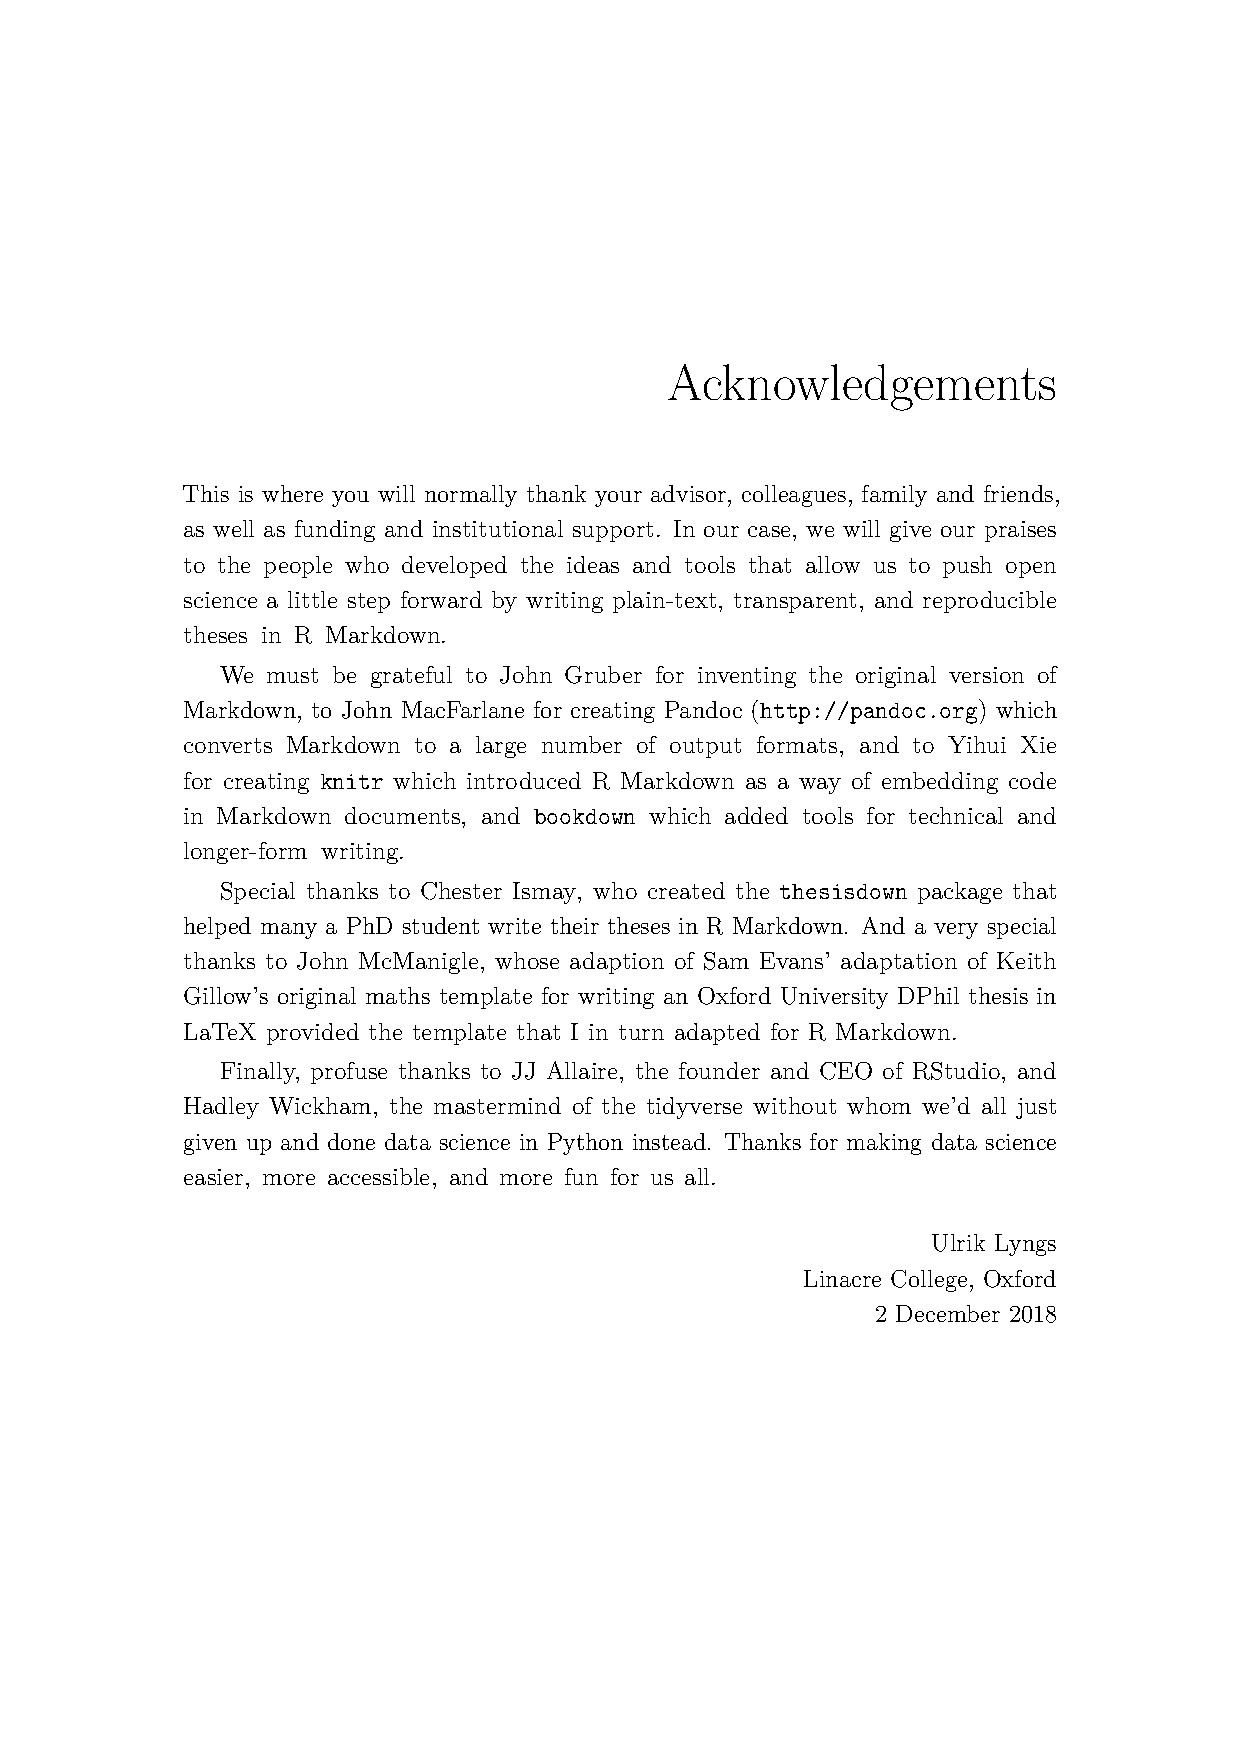
\includegraphics[width=0.32\linewidth]{figures/sample-content/alt_frontmatter_example/split/_000006.pdf}}

\hypertarget{troubleshooting}{%
\chapter{Troubleshooting}\label{troubleshooting}}

This chapter describes common errors you may run into, and how to fix them.

\hypertarget{error-failed-to-build-the-bibliography-via-biber}{%
\section{Error: Failed to build the bibliography via biber}\label{error-failed-to-build-the-bibliography-via-biber}}

This can happen if you've had a failed build, perhaps in relation to RStudio shutting down abruptly.

Try doing this:

\begin{enumerate}
\def\labelenumi{\arabic{enumi}.}
\tightlist
\item
  type \texttt{make\ clean-knits} in the terminal tab (or run \texttt{file.remove(list.files(pattern\ =\ "*.(log\textbar{}mtc\textbar{}maf\textbar{}aux\textbar{}bbl\textbar{}blg\textbar{}xml)"))} in the R console) to clean up files generated by LaTeX during a build
\item
  restart your computer
\end{enumerate}

If this does not solve the problem, try using the \href{https://www.overleaf.com/learn/latex/Bibliography_management_with_natbib}{natbib} LaTeX package instead of \href{https://www.overleaf.com/learn/latex/Articles/Getting_started_with_BibLaTeX}{biblatex} for handling references.
To do this, go to \textbf{index.Rmd} and

\begin{enumerate}
\def\labelenumi{\arabic{enumi}.}
\tightlist
\item
  set \texttt{use-biblatex:\ false} and \texttt{use-natbib:\ true}
\item
  set \texttt{citation\_package:\ natbib} under
\end{enumerate}

\begin{Shaded}
\begin{Highlighting}[]
\FunctionTok{output}\KeywordTok{:}
\AttributeTok{  bookdown:}\FunctionTok{:pdf\_book}\KeywordTok{:}
\AttributeTok{    }\FunctionTok{citation\_package}\KeywordTok{:}\AttributeTok{ natbib}
\end{Highlighting}
\end{Shaded}

\hypertarget{unidade-7}{%
\chapter{Unidade 7}\label{unidade-7}}

\hypertarget{unidade-8}{%
\chapter{Unidade 8}\label{unidade-8}}

\hypertarget{unidade-9}{%
\chapter{Unidade 9}\label{unidade-9}}

\hypertarget{unidade-10}{%
\chapter{Unidade 10}\label{unidade-10}}

\startappendices

\hypertarget{the-first-appendix}{%
\chapter{The First Appendix}\label{the-first-appendix}}

This first appendix includes an R chunk that was hidden in the document (using \texttt{echo\ =\ FALSE}) to help with readibility:

\textbf{In 02-rmd-basics-code.Rmd}

\begin{Shaded}
\begin{Highlighting}[]
\KeywordTok{library}\NormalTok{(tidyverse)}
\NormalTok{knitr}\OperatorTok{::}\KeywordTok{include\_graphics}\NormalTok{(}\StringTok{"figures/sample{-}content/chunk{-}parts.png"}\NormalTok{)}
\end{Highlighting}
\end{Shaded}

\textbf{And here's another one from the same chapter, i.e.~Chapter \ref{code}:}

\begin{Shaded}
\begin{Highlighting}[]
\NormalTok{knitr}\OperatorTok{::}\KeywordTok{include\_graphics}\NormalTok{(}\StringTok{"figures/sample{-}content/beltcrest.png"}\NormalTok{)}
\end{Highlighting}
\end{Shaded}

\hypertarget{the-second-appendix-for-fun}{%
\chapter{The Second Appendix, for Fun}\label{the-second-appendix-for-fun}}


%%%%% REFERENCES
\setlength{\baselineskip}{0pt} % JEM: Single-space References

{\renewcommand*\MakeUppercase[1]{#1}%
\printbibliography[heading=bibintoc,title={\bibtitle}]}


\end{document}
